\documentclass[a4paper,12pt,notitlepage]{book}
\usepackage[italian]{babel}
\usepackage{amsmath, amssymb}
\usepackage{amsthm}
\usepackage{amstext}
\usepackage{array}
\usepackage{graphicx,color,psfrag,pgfplots}
\usepackage[bf,small]{caption}
\usepackage{subfig}
\usepackage{bbm}
\usepackage{wrapfig}
\usepackage{natbib}
\usepackage{listings} % pacchetto per scrivere codice
\usepackage{color}
\usepackage{booktabs}
\usepackage{enumitem}
\usepackage{textcomp}
\usepackage{mathtools}

\usetikzlibrary{patterns,calc,decorations.markings,positioning}

%%%%%%%%%%%%%%PER IL BOX
\usepackage{tikz}
\usetikzlibrary{shapes,positioning,arrows,calc,shadows}
\tikzstyle{abstractbox} = [draw=black, fill=white, rectangle, 
  inner sep=11pt, style=rounded corners] %drop%shadow={fill=gray,opacity=0.8}]
  \tikzstyle{abstracttitle}=[fill=white]  
  \newcommand{\mybox}[3][fill=white]{
    \begin{center}
      \begin{tikzpicture}
        \node [abstractbox, #1] (box)
        {\begin{minipage}{0.95\linewidth}
%           \setlength{\parindent}{2mm}
           \normalsize #2
          \end{minipage}};
        \node[abstracttitle, right=11pt] at (box.north west) {#3};
      \end{tikzpicture}
    \end{center}
  }
%%%%%%%%FINE PER IL BOX


\theoremstyle{plain}
\newtheorem{Teorema}{Theorem}[chapter]

\theoremstyle{definition}
\newtheorem{Definizione}{Definition}[chapter]

\theoremstyle{remark}
\newtheorem{Osservazione}{Observation}[chapter]

\graphicspath{{img/}}

%Comandi personali
\newcommand{\vect}[1]{\mathbf{#1}}
\newcommand{\classe}[1]{\emph{#1}}
\newcommand{\referenza}[1]{[\ref{#1}]}
\newcommand{\referenzaeq}[1]{(\ref{#1})}
\newcommand{\figref}[1]{Fig.\ref{#1}}
\newcommand{\nsp}[1]{\foreach \n in {1,...,#1}{\!}}
\newcommand{\psp}[1]{\foreach \n in {1,...,#1}{\,}}	

\begin{document}

\begin{titlepage}
\begin{center}
    { \scshape 
    Laurea magistrale\\
    in ingegneria matematica\\
    }
\end{center}
\vspace{1.2cm}
\begin{flushleft}
		\Large
		Elaborato di Tesi ...
		\vspace{1.5cm}
\end{flushleft}
\begin{figure}[h]
		\centering
		
\includegraphics[width=0.25\textwidth]{Varie/logo-polimi}
		\vspace{1cm}
\end{figure}
\begin{center}
{ \bfseries  {\Large Titolo progetto di tesi ...}\\
\vspace{0.2cm} }
\end{center}
\vspace{0.4cm}
\begin{flushright}
		\Large
		Progetto svolto da:\\
		Andrea Bortolossi\\
		Matr. 783023\\
		\vspace{1.5cm}
\end{flushright}
\begin{center}
Anno Accademico 2013--2014
\end{center}

\end{titlepage}
\clearpage
\tableofcontents
\chapter{Introduction}
\section{Brief history of VLSI devices}


In 1947 John Bardeen, William Shockley and Walter Brattain (three scientists of Bell Telephone Labs) invented the bipolar transistor and since that crucial point there has been a growth  of the semiconductor industry never known before, with serious impact on the way people work and live today. 

Before reach the functionality and the miniaturization of modern devices, some fundamental steps has been made.
In 1958 was produced the first intagrated circuits (IC)  followed by the introduction of the first MOSFET(1960) and CMOS(1963). Into these inventions the first micro-processor(1971) sank his roots  and since that time until present, an ever-increasing progress has continued, according to the indication of \textit{Moore's Law} (formulated by Gordton Moore in 1965).

These events led microelectronic industry at the doors of the VLSI era (Very-Large-Scale-Integration). Indeed in the last thirty years the benefits of miniaturization have been the key in the evolutionary progress leading to today's computers, wireless units, and comunication systems that offer superior performance, dramatically reduced cost per function, and much reduced physical size.

The large worldwide investment in VLSI technology constitutes a formidable driving force that guarantee the continued progress in IC integration density and speed, for as long as physical principles will allow.

\section{Why FEMOS}

From this point we want start and remark that the aim of numerical simulations is the full comprehension of the physical phenomenon which lies behind the function of modern device. As already underlying this situation became rapidly more important since in the last years devices became more complex and in many cases compact models are insufficent to fully describe the behavoiur of devices.

Even if there's exist many commercial software which are able to resolve different physic situations, it's really difficult satisfy the necessities of industries. A simulator should be more desireable if it  could couple any kind of equations but this is a far ahievement. Modern software are often specialized on precise physic branch. Obviously this strategic choice guarantees more efficiency but it implies a lost in generality. The conseguence is that the work of the model analyst became harder when he have to afford problems located in the middle of different phenomenon. 

Consider for a moment to analyse the funcionality of a new device, which its electric behaviour is strong influeced by its mechanic response. Basically you are interested to the resolution of Maxwell's law  (which is well performed by SDEVICE simulator) and the Navier-Lam\`e equations (which is well performed by COMSOL simulator). Now the question is: how to put in comunication the different outputs?
Take into account that it's not possbile known precisely how the above programs resolves the equations, which implies a relevant risk when you decide to combine the solutions. 
In other words the development of an own code is at least desirable and possibly helpful. The main advantage is the total control on simulation procedure and the possibility of fully customize. Although the major drawback is that the improvement of a personal code needs time and human resources, which in many cases are not avaible.   

The FEMOS project (\textit{Finite Element Method Oriented Solver}) sinks its motivations in the above framework. The main intention is to solve different physics aspects and give a more precise description of devices with a single output. The complexity of this achievement guarantees a continuum source of physic, numerical and programming challenges. 
Between them, even if modern devices present innovative and unexpected behaviour, we can't avoid the treatment of the classical semiconductor devices from the simulation possibilties of FEMOS.
This thesis found its origin in the development of this achievement, but as subject covered a spread wide area in terms of models and kind of devices, we decide to focus on precise points which we present here:
\begin{itemize}
\item development of a finite element based simulator for semiconductor devices which deals with multiple generation/recombination and mobility models;
\item check solutions obtained against commercial software (SDEVICE);
\item definition and implementation of a new way to compute the current density inside the device;
\item extension of the residual method presented in \textcolor{red}{referenza} for the 3D case;
\item evaluation of the possibility to extend the residual method at the computation of the current density inside the device.
\end{itemize}


\clearpage
\chapter{Semiconductor model}

In this chapter we shall present the basic physics properties of semiconductor material accordingly with the quantum mechanics theory \citep{ModernVLSIdevices}. The Drift-Diffusion model is then presented.

\section{Basic Device Physics}

This section covers the basic concepts of semiconductor device physics. As the most used material in the fabrication of VLSI devices is silicon, in the follow we will focus on it.

\subsection{Intrinsic semiconductor}
In a silicon crystal each atom has four valence electrons to share with its four nearest neighboring atoms. The valence electrons are shared in a paired configuration called a covalent bond. The most important result of the application of quantum mechanics to the description of electrons in a solid is that the allowed energy levels of electrons are grouped into bands. The bands are separated by regions of energy that the electrons in the solid cannot possess: forbidden gaps. The highest energy band that is completely filled by electron at 0[K] is called the \textit{valence band} ($E_V$). The next higher energy band, separated by a frobidden gap from the valence band, is called the \textit{conduction band} ($E_C$).

\begin{figure}[!h]
\centering
\subfloat[][Metal]
{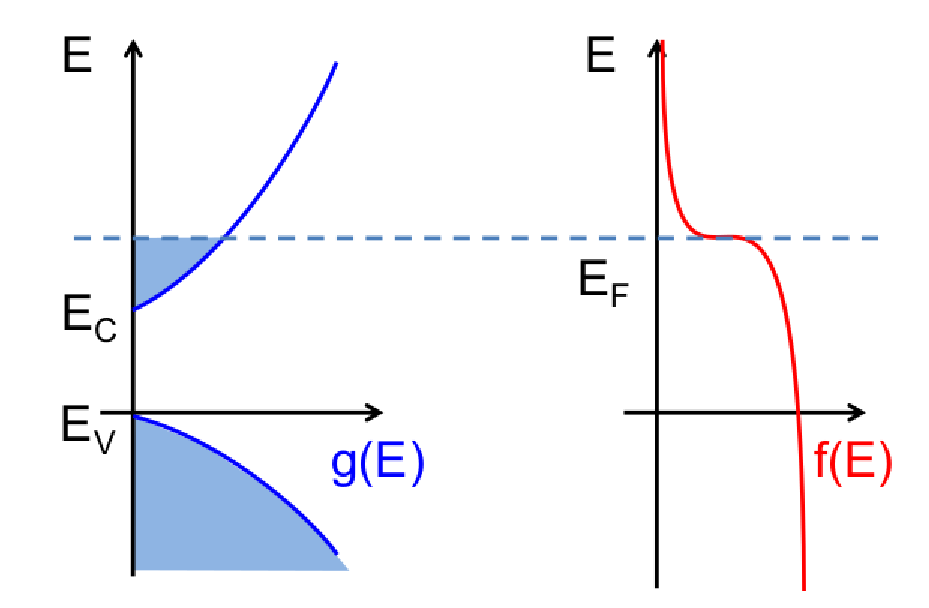
\includegraphics[width=.45\textwidth]{SemiconductorModel/BandeMetalli.eps}}
\psp{5}
\subfloat[][Insulator]
{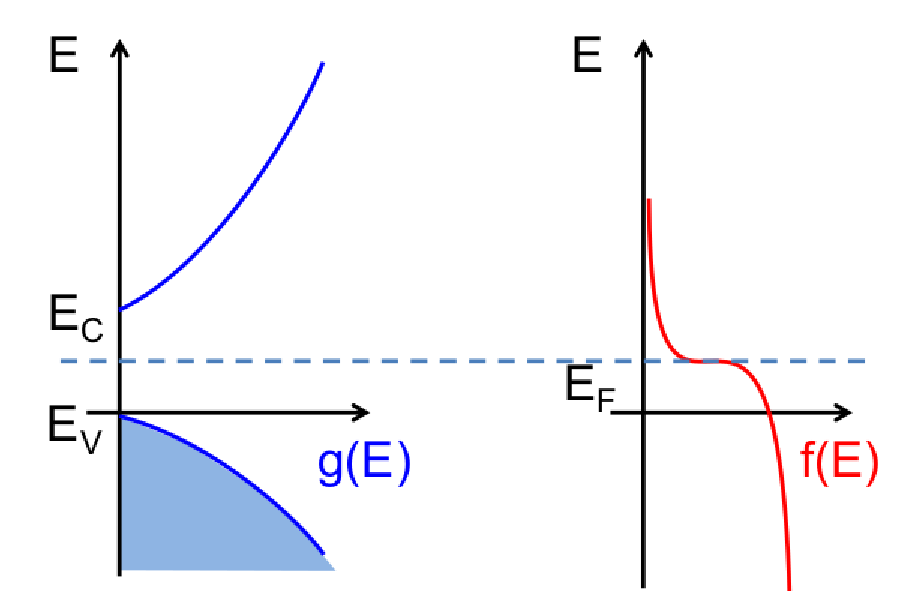
\includegraphics[width=.45\textwidth]{SemiconductorModel/BandeSemiconduttori.eps}}
\caption{Two typical examples of state density occupation (g(E)) and probability distribution (f(E)).  }
\end{figure}

Because in silicon the band gap is on the order of 1 [eV], at room temperature a small fraction of the electrons are excited into the conduction band, leaving behind vacancies (called \textit{holes}) in the valence band.
In contrast, an insulator has a much larger forbidden gap making room-temperature conduction virtually impossible, while metals have partially filled conduction bands even at absolute zero temperature, this make them good conductors at any temperature. 

A suitable formulation of che carrier concentration which is given, for electrons, by the follow integral:
\begin{equation}
\label{eq: carrier densiy integral}
n = \int_{E_c}^\infty g(E)f(E) \, dE
\end{equation}
With $g(E)dE$ we indicate the number of electronic states per unit volume with an energy between $E$ and $E+dE$ in the conduction band and $f(E)$ is a suitable probability ditribution.

The energy distribution of electrons in a solid is governed by the laws of Fermi-Dirac statistics. For a system in thermal equilibrium, the principal result of these statistics is the \textit{Fermi-Dirac distribution function}, which gives the probability that an electronic state at energy E is occupied by an electron,
\begin{equation}
\label{eq: fermi dirac distribution}
f_D(E) = \dfrac{1}{1+exp\left(\dfrac{E-E_f}{k_BT}\right)} 
\end{equation}
here $k_B=1.38\times10^{-23}[J/K]$ is Boltzmann's constant, $T$ is the absolute temperature and $E_f$ is the \textit{Fermi level}.

\begin{Definizione}
The Fermi level ($E_f$) is the energy at which the probability of occupation of an energy state by an electron is exactly one-half.
\end{Definizione}

In most cases when the energy is at least several $k_BT$ above or below the Fermi level \referenzaeq{eq: fermi dirac distribution} can be approximated with the Maxwell-Boltzmann statistics for classical particles, which read as follows:

\begin{equation}
\label{eq: maxwell distribution}
f_D(E)\simeq f_{MB}(E) = 
\begin{cases}
exp\left(-\dfrac{E-E_f}{KT}\right) & E\gg E_f \\
1-exp\left(-\dfrac{E_f-E}{KT}\right) & E \ll E_f
\end{cases}
\end{equation}

Fermi level plays an essential role in characterizing the equilibrium state of a stystem, it is important to keep in mind the sequent observation.

\begin{Osservazione}
When two systems are in thermal equilibrium with no current flow between them, their Fermi levels must be equal, in other words for a continuous region of metals and/or semiconductors in contact, the Fermi level at thermal equilibrium is flat (spatially constant throughout the region).
\end{Osservazione}

 In general \referenzaeq{eq: carrier densiy integral} is a Fermi integral of the order $1/2$ and must be evaluated numerically. In the case of non-degenerate semiconductor, Fermi levels stay at least $3KT/q$ below the edge of the conduction band (for holes we consider the same approximation above the valence band).  The Fermi-Dirac distribution can be approximated by the Maxwell-Boltzmann distribution and \referenzaeq{eq: carrier densiy integral} can be solved in the analytically way, obtaining,

\begin{align}
n & = N_c exp\left(-\dfrac{E_c-E_f}{KT}\right) \label{eq: n density fd}\\
p & = N_v exp\left(-\dfrac{E_f-E_v}{KT}\right)  \label{eq: p density fd}
\end{align}

where $N_c$ and $N_v$ are the \textit{effective density of states}.
In intrisic semiconductor $n=p$ and the \textit{intrinsic Fermi level} $E_i$ can be calculated using equations \referenzaeq{eq: n density fd} and \referenzaeq{eq: p density fd} as:

\begin{equation}
\label{eq: midgap equilibrium}
E_i=E_f=\dfrac{E_c+E_v}{2} - \dfrac{KT}{2}ln\left(\dfrac{N_c}{N_v}\right)
\end{equation}

By replacing \referenzaeq{eq: midgap equilibrium} in \referenzaeq{eq: n density fd} we have the expression of the intrinsic carrier concentration $n_i=n=p$:


\begin{equation}
\label{eq: ni equilibrium NcNv}
n_i = \sqrt{N_cN_v}exp\left(-\dfrac{E_g}{2KT}\right)
\end{equation}

\begin{Osservazione}
Since the thermal energy, $k_BT$ is muc smaller than the usual semiconductor bandgap $E_g$, the intrinsic Fermi level is very close to the midpoint between the conduction band and the valence band.
\end{Osservazione}

Equations \referenzaeq{eq: n density fd} and \referenzaeq{eq: p density fd} can be rewritten in terms of the intrinsic carrier density ($n_i$) and energy ($E_i$) :

\begin{align}
n & = n_i exp\left(\dfrac{E_f-E_i}{KT}\right) \label{eq: n density mb}\\
p & = n_i exp\left(\dfrac{E_i-E_f}{KT}\right)  \label{eq: p density mb}
\end{align}

Finally we remark a fundamental and useful relation holds at the thermical equilibrium

\begin{equation}
\label{eq: legge di azione di massa}
np=n_i^2
\end{equation}

this relation is usually note as \textit{mass action law}.

One of the most used graphical tool for the anlysis of the functionality of devices is the band diagram \figref{fig: band diagram}, which summarizes the informations presented above.
\begin{figure}[!h]
\centering
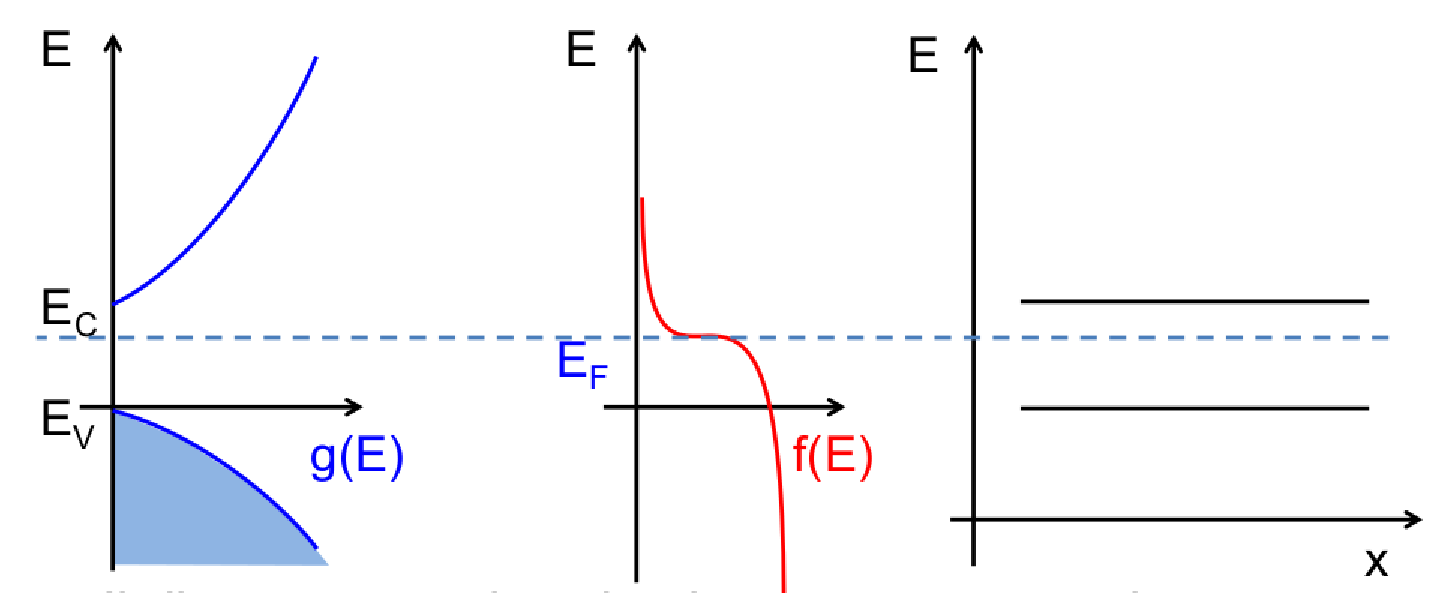
\includegraphics[width=.8\textwidth]{SemiconductorModel/DiagrammaBande.eps}
\caption{Construction of tha band diagram.}
\label{fig: band diagram}
\end{figure}

\subsection{Extrinsic semiconductor}
At room temperature intrinsic semiconductor has an extremely low free-carrier concentration, therefore, its resistivity is very high. In order to make semiconductor a better conductor it's usual add impurities atoms which introduce additional energy levels in the forbidden gap: these impurities are easily ionized adding either electrons to the conduction band or holes to the valence band. Here the electrical conductivity is dominated by the type and concentration of the impurity atoms.

In the case of silicon two are the types of impurities which are electrically active: those from column V such as arsenic or phosphorus, and those from column III such as boron or indium.

A column-V atom in a silicon lattice tends to have one extra electron loosely bonded after forming covalent bonds with other silicon atoms. In most cases, the thermal energy at room temperature is sufficient to ionize the impurity atom and free the extra electron to the conduction band. Such type of impurities are called \textit{donors}; they become positively charged when ionized. Silicon material doped with column-V impurities or donors is called \textit{n-type} silicon.

A column-III impurity atom in a silicon lattice tends to be deficient by one electron when forming covalent bonds with other silicon atoms. Such an impurity atom can also be ionized by accepting an electron from the valence band, which leaves a free-moving hole that contributes to electrical conduction. These impurities are called \textit{acceptors}: they become negatively charged when ionized. Silicon material doped with column-III impurities or acceptors is called \textit{p-type} silicon.

A p-type or an n-type is named as \textit{extrinsic} silicon.
In terms of the energy-band diagrams, donors add allowed electron states in the bandgap close to the conduction-band edge, while acceptors add allowed states just above the valence-band edge.

In contrast to intrinsic silicon, the Fermi level in an extrinsic silicon is not located at the midgap. The Fermi level in n-type silicon moves up towards the conduction band while in p-type silicon moves down towards the valence band.
The exact position of the Fermi level depends on both the ionization energy and the concentration of dopants. For example, for an n-type material with a donor impurity concentration, $N_d$, the charge neutrality condition requires that
\begin{equation}
\label{eq: equilibrium charge in n-type}
n = N_d^+ + p
\end{equation}
 where $N_d^+$ is the density of ionized donors.  Similarly for a p-type material with acceptor impurity concentration $N_a$ we have
\begin{equation}
\label{eq: equilibrium charge in p-type}
p = N_a^- + n
\end{equation}
 
 For the sake of simplicity we consider in this work that at room temperature all impurties are ionized ($N_d = N_d^+$ and $N_a = N_a^-$). Typcally the magnitude of impurities is between $10^{16}\ast 10^{20} [cm^{-3}]$, while the usual intrinsic carrier concentration is almost $10^{10}[cm_3]$, for this reason we can approximate the equilibrium densities concentration:
  
\begin{equation}
\begin{array}{ll}
n \simeq N_d & p \simeq \dfrac{n_i^2}{N_d} \\ \\
p \simeq N_a & n \simeq \dfrac{n_i^2}{N_a}
\end{array}
\end{equation}

 Take into account this approximation and substituting \referenzaeq{eq: n density fd} and \referenzaeq{eq: p density fd} in \referenzaeq{eq: equilibrium charge in n-type} and \referenzaeq{eq: equilibrium charge in p-type}, solving the algebraic equationwe have
 
 \begin{align}
 E_c-E_f = KTln\left(\dfrac{N_c}{N_d}\right)  \label{eq: Ef in n-type}\\
 E_f-E_v= KTln\left(\dfrac{N_v}{N_a}\right) \label{eq: Ef in p-type}
 \end{align}

Equation \referenzaeq{eq: legge di azione di massa} is indipendent of the dopant type and Fermi level position.
Instead of using $N_c$, $N_v$ and referring to $E_c$ and $E_v$ equation \referenzaeq{eq: Ef in n-type} and \referenzaeq{eq: Ef in p-type} can be written in a more useful form in terms of $n_i$ and $E_i$ defined by equations \referenzaeq{eq: ni equilibrium NcNv} and \referenzaeq{eq: midgap equilibrium}:

 \begin{align}
 E_f-E_i = KTln\left(\dfrac{N_d}{n_i}\right)  \label{eq: Ef in n-type Ei} \\
 E_i-E_f = KTln\left(\dfrac{N_a}{n_i}\right)  \label{eq: Ef in p-type Ei} 
 \end{align}

\begin{Osservazione}
The distance between the Fermi level and the intrinsic Fermi level near the midgap is a logarithmic function of doping concentration.
\end{Osservazione}

As a consequences:
\begin{itemize}
\item non linearity relations between potential and desities,
\item exponential dependence of densities from potential.
\end{itemize}

\begin{figure}[!h]
\centering
\subfloat[][n-type]
{\begin{tikzpicture}
[scale=1.0]
\def\Ecxa{0.0}
\def\Ecya{2}
\def\Ecxb{3}
\def\Ecyb{2}

\def\Evxa{\Ecxa}
\def\Evya{0}
\def\Evxb{\Ecxb}
\def\Evyb{0}

\def\Efxa{\Ecxa}
\def\Efya{1.7}
\def\Efxb{\Ecxb}
\def\Efyb{1.7}

\def\Eixa{\Ecxa}
\def\Eiya{1}
\def\Eixb{\Ecxb}
\def\Eiyb{1}

\node at (\Ecxb+0.5,\Ecyb){$E_C$};
\node at (\Evxb+0.5,\Evyb){$E_V$};
\node at (\Efxa-0.5,\Efya){$E_f$};
\node at (\Eixa-0.5,\Eiya){$E_i$};

\draw[ultra thick](\Ecxa,\Ecya)--(\Ecxb,\Ecyb);
\draw[ultra thick](\Evxa,\Evya)--(\Evxb,\Evyb);
\draw[ultra thick,dashed](\Efxa,\Efya)--(\Efxb,\Efyb);
\draw[dashed](\Eixa,\Eiya)--(\Eixb,\Eiyb);
\end{tikzpicture}}
\psp{20}
\subfloat[][p-type]
{\begin{tikzpicture}
[scale=1.0]
\def\Ecxa{0.0}
\def\Ecya{2}
\def\Ecxb{3}
\def\Ecyb{2}

\def\Evxa{\Ecxa}
\def\Evya{0}
\def\Evxb{\Ecxb}
\def\Evyb{0}

\def\Efxa{\Ecxa}
\def\Efya{0.3}
\def\Efxb{\Ecxb}
\def\Efyb{0.3}

\def\Eixa{\Ecxa}
\def\Eiya{1}
\def\Eixb{\Ecxb}
\def\Eiyb{1}

\node at (\Ecxb+0.5,\Ecyb){$E_C$};
\node at (\Evxb+0.5,\Evyb){$E_V$};
\node at (\Efxa-0.5,\Efya){$E_f$};
\node at (\Eixa-0.5,\Eiya){$E_i$};

\draw[ultra thick](\Ecxa,\Ecya)--(\Ecxb,\Ecyb);
\draw[ultra thick](\Evxa,\Evya)--(\Evxb,\Evyb);
\draw[ultra thick,dashed](\Efxa,\Efya)--(\Efxb,\Efyb);
\draw[dashed](\Eixa,\Eiya)--(\Eixb,\Eiyb);
\end{tikzpicture}}
\caption{Band diagrams of estrinsic silicon.}
\label{fig: Band diagrams of estrinsic silicon}
\end{figure}

\subsection{Densities at nonequilibrium condition}

In VLSI device operation a nonequilibrium sistuations is often possible: the densities of one or both types of carriers depart from their equilibrium values given by \referenzaeq{eq: n density mb} and \referenzaeq{eq: p density mb}.
In particular, the minority carrier concentration can be easily overwhelmed by injection from neighboring regions. Under these circumstances, while the electrons and holes are in local equilibrium with themselves, they are not in equilibrium with each other. In order to extend the relationship between Fermi level and densities discussed above, we can introduce separate Fermi levels for electrons and holes. They are called \textit{quasi Fermi levels} defined as $E_{fn}$ and $E_{fp}$ replacing equation \referenzaeq{eq: n density mb} and \referenzaeq{eq: p density mb}:

\begin{align}
n & = n_i exp\left(\dfrac{E_{fn}-E_i}{k_BT}\right) \label{eq: non eq n density mb}\\
p & = n_i exp\left(\dfrac{E_i-E_{fp}}{k_BT}\right)  \label{eq: non eq p density mb}
\end{align}

In non equilibrium condition quasi Fermi levels have a similar physical interpretation in terms of the state occupancy as the Fermi level.
\begin{Osservazione}
The electron density in the conduction band can be calculated using $E_{fn}$, and the hole density in the valence band using $E_{fp}$.
\end{Osservazione}

\subsection{Carrier transport in semiconductor}
\label{sec: carrier transport}

Carrier transport or current flow in silicon is driven by two different mechanisms:
\begin{itemize}
\item the \textbf{drift} of carriers, which is caused by the presence of an electric field;
\item the \textbf{diffusion} of carriers, which is caused by and electron or hole concentration gradient.
\end{itemize}

\subsubsection{Drif current - Ohm's law}

When an electric field is applied to a media, the free carriers are accelerated and acquire a drift velocity superimposed upon their random thermal motion.

\begin{Osservazione}
The drift velocity of holes ($h$) is in the direction of the applied field, and the drift velocity of electrons ($e$) is opposite to the field.
\end{Osservazione}

The velocity of the carriers does not increase indefinitely under field acceleration, since they are scattered frequently and lose their acquired momentum after each collision.
During their motion throughout the lattice structure, carriers travel at an average speed definded as
\begin{equation}
\label{eq: velocities}
\vect{v}_d^e = - \dfrac{q\vect{E}\tau_e}{m_e}  \psp{20} 
\vect{v}_d^h = + \dfrac{q\vect{E}\tau_h}{m_h}
\end{equation}

where $q=1.602e^{-19}[C]$ is the elementary charge, $\vect{E}$ the electric field, $\tau_\eta$ the average time of flight of the carrier between two consecutive interactions with the atoms of the lattice and $m_\eta$ is the effective mass.
The coefficient $q\tau_\eta / m_\eta$ characterizes how quickly a carrier can move through the lattice and it's well known as carrier mobility $[m^2V^{-1}s^{-1}]$.
In general, to include different contributions to the mobility \textit{Matthiessen's rule} is used:
\begin{equation}
\dfrac{1}{\mu} = \dfrac{1}{\mu_L} + \dfrac{1}{\mu_I} + \cdots
\end{equation}
where $\mu_L$ and $\mu_I$ correspond to the lattice and impurity scattering limited components of mobility (for a more detailed description of mobility models see \cite{ModernVLSIdevices}). 

Therefore the drift electron, hole, current density, reads as follows:

\begin{align}
\vect{J}_n =& -qn\vect{v}_d^n = qn\mu_n\vect{E}   = \sigma_n\vect{E} \label{eq: drift electron} \\ 
\vect{J}_p =& +qp\vect{v}_d^p = qp\mu_p\vect{E} = \sigma_p\vect{E} \label{eq: drift hole}
\end{align}

The scalar coefficient $qn\mu_n(qp\mu_p)$ is often summerized by the electron (hole) conductivity $\sigma_n(\sigma_p)$. 

Relations \referenzaeq{eq: drift electron} and \referenzaeq{eq: drift hole} expresses the well known \textit{Ohm' law} stating that the current density is directly proportional to the applied electric field.


\subsubsection{Diffusion current - Fick's law}

In semiconductor devices it's usual have different profiles of dopant in order to allow particular behaviors, this implies a not uniform concentration of carriers which they also diffuse as a result of the concentration gradient. This leads to an additional current contribution accordingly to the \textit{Fick's law}:
\begin{align}
\vect{J}_n = -D_n(-q\nabla n) \label{eq: diff electron}\\
\vect{J}_p = -D_p(+q\nabla p) \label{eq: diff hole}
\end{align}

The proportionally constants $D_n$ and $D_p$ are called the electron and hole diffusion coefficients and have units of $[cm^2s^{-1}]$. Physically, both drift and diffusion are closely associated with the random thermal motion of carriers and their collisions with the silicon lattice in thermal equilibrium. A simple relationship between the diffusion coefficient and the mobility is the well known \textit{Einstein relation}:
\begin{equation}
D_\eta = \dfrac{k_BT}{q}\mu_\eta
\end{equation}

\subsubsection{Drift-Diffusion transport equations}
\label{subsub:driftdiffusion transport}

By considering \referenzaeq{eq: drift electron}, \referenzaeq{eq: drift hole}, \referenzaeq{eq: diff electron} and \referenzaeq{eq: diff hole}, the total electron and hole current densities are:

\begin{align}
\vect{J}_n &= qn\mu_n\vect{E} + qD_n\nabla n  \label{eq: drift diff electron}\\ 
\vect{J}_p &= qp\mu_p\vect{E} - qD_p \nabla p \label{eq: drift diff hole}
\end{align}
The total conduction current density is $\vect{J}=\vect{J}_n+\vect{J}_p$.

We remark that these constitutive laws can be rewritten in two other ways highlighting different physical explanations of the same phenomenon. Moreover these reinterpreations  give different start points for the discrete solver algorithm.

Considering that electric field is related to the scalar potential as:
\begin{equation}
\label{eq: relazione pot electric}
\vect{E}  = -\nabla \varphi
\end{equation}

the current densities can be :

\begin{align}
\vect{J}_n &= -qn\mu_n\left(\nabla \varphi - \dfrac{k_BT}{qn}\nabla n \right) \label{eq: Jn DD} \\ 
\vect{J}_p &= -qp\mu_p\left(\nabla \varphi+ \dfrac{k_BT}{qp} \nabla p \right) \label{eq: Jp DD}
\end{align}

Considering equations \referenzaeq{eq: non eq n density mb} and \referenzaeq{eq: non eq p density mb} the above can be written as:

\begin{align}
\vect{J}_n = -qn\mu_n\nabla \varphi_n \label{eq: Jn qf}\\
\vect{J}_p = -qp\mu_p\nabla \varphi_p \label{eq: Jp qf}
\end{align}

With these equations we underlying an important aspect which occur in semiconductor material:
\begin{Osservazione}
The current density is proportional to the gradient of the quasi Fermi potential.
\end{Osservazione}

The third way to represent the current density is based on \textit{Slotboom variables}. In 1973 Jan Slotboom proposed this change in variables for the two-dimensional numercal simulation of a bipolar transistor:

\begin{align}
u_n &= n_iexp\left(-\dfrac{\varphi_n}{V_{th}} \right) \label{eq: un slotboom} \\
u_p &= n_iexp\left(\dfrac{\varphi_p}{V_{th}} \right) \label{eq: up slotboom} 
\end{align}

where $V_{th}=k_BT/q$. Using the above equations into \referenzaeq{eq: drift diff electron} and \referenzaeq{eq: drift diff hole} we obtain:

\begin{align}
\vect{J}_n &= qD_n exp\left(\dfrac{\varphi}{V_{th}}\right) \nabla u_n \label{eq: Jn slotboom} \\
\vect{J}_p &= -qD_p exp\left(-\dfrac{\varphi}{V_{th}}\right)  \nabla u_p \label{eq: Jp slotboom}
\end{align}

This interpretation results is:
\begin{Osservazione}
The drift-diffusion current density in a semiconductor, is a totally diffusive flux of a new kind of carrier and diffusivity coefficient. 
\end{Osservazione}


\section{Drift Diffusion Model for semiconductor}
\label{section: dd model for semi}

Simulations on integrated devices works on several different scale, the \textit{Drift Diffusion model} (DD) is the most widely used mathematical tool for industrial simulaiton of semiconductor devices. In this section we'll show how is possible to deduce the DD model.

\subsection{Drift Diffusion formulation}
 The system of Maxwell equations describes the propagation of electromagnetic signal in a medium:

\begin{align}
\nabla \times \vect{H} & =  \vect{J} + \dfrac{\partial \vect{D}}{\partial t} \label{eq: magnetic equation} \\ 
\nabla \times \vect{E} & =  - \dfrac{\partial \vect{B}}{\partial t} \label{eq: ampere law}\\ 
\nabla \cdot \vect{D} & =  \rho \label{eq: gauss law}\\ 
\nabla \cdot \vect{B} &  =  0 \label{eq: no magetic charge law}
\end{align}

we complete the system with the following set of constitutive laws that characterize the electromagnetic properties of the medium:

\begin{equation}
\begin{array}{rcl}
\vect{D} & = & \epsilon \vect{E} \\
\vect{B} & = & \mu_m \vect{H} \label{eq: magnetic costitutive}
\end{array}
\end{equation}

where $\epsilon$ is the material dielectric permettivity $[F cm^{-1}]$ and $\mu_m$ is the magnetic permeability $[H cm^{-1}]$. Since $\nabla \cdot (\nabla \times \vect{A})=0$ for any vector $\vect{A}$, \referenzaeq{eq: no magetic charge law} is satisfied by introducing a vector potential $\vect{A}$ such that $\vect{B}= \nabla \cdot \vect{A}$. We replace it in \referenzaeq{eq: ampere law} and we obtain

\begin{equation}
\nabla \times \left( \vect{E} + \dfrac{\partial \vect{A}}{\partial t} \right) = 0.
\end{equation}

From this we can state that exist a scalar potential $\varphi$ such that

\begin{equation}
\label{eq: potenziale scalare}
\vect{E} + \dfrac{\partial \vect{A}}{\partial t} = -\nabla \varphi
\end{equation}


We multiply \referenzaeq{eq: potenziale scalare} by $\epsilon$, we apply the divergence operator and we obtain using \referenzaeq{eq: relazione pot electric}, \referenzaeq{eq: magnetic costitutive} and \referenzaeq{eq: gauss law}

\begin{equation}
\rho + \dfrac{\partial \vect{A}}{\partial t}  = -\nabla \cdot (\epsilon \nabla \varphi)
\end{equation}

We now assume that $\dfrac{\partial \vect{A}}{\partial t} = 0$ (quasi static approximation) and we obtain the \textit{Poisson Equation}

\begin{equation}
\label{eq: Poisson equation}
\nabla \cdot (\epsilon \nabla \varphi) = \rho.
\end{equation} 
	
	We apply the divergence operator on the equation \referenza{eq: magnetic equation}  and we get the \textit{Continuity Equation}

\begin{equation}
\dfrac{\partial \rho}{\partial t} + \nabla \cdot \vect{J}  =  0 \end{equation} 




To close the above system we need to specify the mathematical form of the electric charge density ($\rho$) and the electric conduction current density ($\vect{J}$).
As we introduced in the preview section, devices are usually formed by extrinsic semiconductor and this causes the presence in the lattice of two kind of charge:

\begin{itemize}
\item free charge ($\rho_{free}$) (free electron and holes carriers),
\item fixed charge ($\rho_{fixed}$) (ionoized dopant impurities).
\end{itemize} 

\begin{equation}
\label{eq: charge balance}
\rho = \underbrace{q(p-n)}_{\rho_{free}} +\underbrace{q(N_D^+-N_A^-)}_{\rho_{fixed}}
\end{equation}

 Notice that we assume $N_D^+$ and $N_A^-$ time invariant ($\partial N_D^+ / \partial t=\partial N_A^- / \partial t = 0$).

 Accordingly with the preview hypotesis and replacing \referenzaeq{eq: charge balance}, \referenzaeq{eq: drift diff electron} and \referenzaeq{eq: drift diff hole}, we can split the continuity equation into the contribute of electrons and holes, the DD model formulation looks as follows:
 
\begin{equation}
\label{eq: full problem}
\left\{
\begin{array}{rcl}
\nabla \cdot (-\epsilon \nabla \varphi) & = & q(p-n+N_D^+-N_A^-)\\ \\
-q\dfrac{\partial n}{\partial t} + \nabla \cdot ( - q\mu_n n \nabla \varphi + qD_n \nabla n )& = & qR\\ \\
q\dfrac{\partial p}{\partial t} + \nabla \cdot (- q\mu_p p \nabla \varphi - qD_p \nabla p )& = & -qR 
\end{array}
\right.
\end{equation}

The system is an incompletely parbolic initial value/boundary problem in three scalar unkown dependent variables $\varphi(\vect{x},t)$, $n(\vect{x},t)$ and $p(\vect{x},t)$. Notice that the problem is a nonlinearly coupled system of PDE's, because of the presence of the drift terms ($n\nabla \varphi$ and $p \nabla 	\varphi$). 

From Maxwell equations we are able to guarantee only that $\vect{J}$ is a solenoidal field, we can't say nothing about the properties of $\vect{J_n}$ and $\vect{J_p}$. We can interpret $R(\vect{x},t)$ as the net rate of generation and recombination.

The stationary form can be easily derivate from \referenzaeq{eq: full problem} by not considering the temporal derivative.

%\begin{equation}
%\label{eq: stationary problem}
%\left\{
%\begin{array}{rcl}
%\nabla \cdot (-\epsilon \nabla \varphi) & = & q(p-n+N_D^+-N_A^-) \\ \\
%\nabla \cdot ( - q\mu_n n \nabla \varphi + qD_n \nabla n )& = & qR \\ \\
%\nabla \cdot (- q\mu_p p \nabla \varphi - qD_p \nabla p )& = & -qR
%\end{array}
%\right.
%\end{equation}




\subsection{Generation and Recombination phenomenon}
\label{subsection: RG}

The modelling of $R(\vect{x},t)$ is one of the most important feature due to the important role in determining the current-voltage characteristic of devices.
 
It's important to keep in mind that electrons and holes are in continuos fluctuation due to their thermal energy, but the macroscopic result of such a process at equilibrium is that the net recombination rate is identically zero at each point and at each time level. Therefore our interest is to analyze the deviations from this condition. 

In every moment the system try to mantain the equilibrium, so it's important underlying that the response with a recombination event happens in order to neutralize an excess of charge, while generation event are usually due to thermal agitation or an external input source.

The phenomenological model for the net recombination rate $R$ is often given by the sequent formulation:
\begin{equation}
\label{eq: generic RG}
R(n,p) = (pn-n_i^2)F(n,p)
\end{equation}
where $F$ is a function modelling the specific recombination/generation (R/G) event.

In the following we present the classical theory about three kind of contribute. 

\subsubsection{Shockley-Read-Hall recombination (SRH)}

Electron and hole generation and recombination can take place directly between the valence band and the conduction band, or inderactly via trap centers in the energy gap (we indicate with $E_T$ the energy level at where these traps live). The latter category includes Shockley-Read-Hall phenomena (SRH), more precisely SRH rate is a two-particle process which matematically expresses the probality that:
\begin{itemize}
\item[$R_{SRH}$] an electron in the conduction band neutralizes a hole at the valence band through the mediation of an unoccupied trapping level located in the energy gap,
\item[$G_{SRH}$] an electron is emitted from the valence band to the conduction band, through he mediation of an unoccupied trapping level located in the energy gap.
\end{itemize}

The following expression is usually employed for the modulating function $F$:

\begin{equation}
F_{SRH}(n,p) = \dfrac{1}{\tau_n\left(p+n_i cosh\left(\dfrac{E_T}{k_BT} \right) \right)+\tau_p\left(n+n_i cosh\left(\dfrac{E_T}{k_BT}\right) \right)}
\end{equation}

the quantiaties $\tau_n$ and $\tau_p$ are called \textit{carrier lifetimes} and are phisically defined as the reciprocals of the capture rates per single carrier associated with the energy trap distribution within the semiconductor energy gap. Their typical order of magnitude lies in the range $10^{-3}\mu s\div 1 \mu s$.

\begin{table}[!h]
\centering
\begin{tabular}{cccc}
\toprule
Parameter & Unit & Electrons & Holes \\
\midrule
$\tau$ & s & $1.0\times 10^{-5}$ & $3.0 \times 10^{-6}$\\
$E_T$ & eV & 0.0 & 0.0\\
\bottomrule
\end{tabular}
\caption{List of parameters in the electron and hole mobility models including scattering from lattice thermal vibrations}
\end{table}

\subsubsection{Auger recombination (AU)}

Auger R/G is a three-particle process and take place directly between the valence band and the conduction band. We distinguish four cases which depend to the kind of carriers involved in the phenomena:
\begin{itemize}
\item[$R_{AU}^{2n,1p}$] a high-energy electron in the conduction band moves to the valence band where it neutralizes a hole, transmitting the excess energy to another electron in the conduction band;
\item[$G_{AU}^{2n,1p}$] an electron in the valence band moves to the conduction band by taking the energy from a high energy electron in the conduction band and leaves a hole in the valence band;
\item[$R_{AU}^{2p,1n}$] an electron in the conduction band moves to the valence band where it neutralizes a hole, transmitting the excess energy to another hole in the valence band;
\item[$G_{AU}^{2p,1n}$] an electron in the valence band moves to the conduction band by taking the energy from a high energy hole in the valence band and leaves a hole in the valence band.
\end{itemize}

The following expression is usually employed for the modulating function $F$:

\begin{equation}
F_{AU}(n,p) = C_nn+C_pp
\end{equation}

where the quantitaties $C_n$ and $C_p$ are the so called  Auger capture coefficients tipically of the order of magnitude of $10^{-25}[cm^6s^{-1}]$.
Note that Auger R/G is relevant only when both carrier densities attain high values.

\begin{table}[!h]
\centering
\begin{tabular}{ccc}
\toprule
Parameter & Unit & Magnitude \\
\midrule
$C_n$ & $cm^6s^{-1}$ & $2.9 \times 10^{-31}$ \\
$C_p$ & $cm^6s^{-1}$ & $1.028 \times 10^{-31}$ \\
\bottomrule
\end{tabular}
\caption{List of parameters in the electron and hole Auger generation/recombination model.}
\end{table}

\subsubsection{Impact ionization (II)}

The impact ionization mechanism is a three-particle generation  process and it is dissimilar from the previously phenomenon because we can't express its contribute with a relation like \referenzaeq{eq: generic RG}. The high energy carrier generation is triggered by the presence of very high electric fields. Due to these fields an electron could gains enough energy to excite an electron-hole pair out of a silicon lattice bond. Then the process can be repeated until an avalanche of generated carriers is produced within the region.
There are several different models for the II generation, inside our code we implemented the van Overstraeten - de Man \textcolor{red}{referenza manuale sdevice} model based on the Chynoweth law \textcolor{red}{referenza dentro sdevice}:
\begin{equation}
G_{II}(n,p)= \alpha_n n |\vect{v}_n| + \alpha_p p |\vect{v}_p|
\end{equation}

where:

\begin{equation}
\alpha(E_{ava}) = \gamma exp\left(-\dfrac{\gamma b}{E_{ava}} \right)
\end{equation} 
\begin{equation}
\gamma = \dfrac{tanh\left(\dfrac{\hbar \omega_{op}}{2k_BT_0} \right) }{tanh\left(\dfrac{\hbar \omega_{op}}{2k_BT} \right)}
\end{equation}

The factor $\gamma$ with the optical phono energy $\hbar \omega_{op}$ expresses the temperature dependence of the phonon gas against which carriers are accelerated.
$E_{ava}$ is the driving force which takes into account how the electric field influence the generation event. There are two possibilties to compute this quantity:
\begin{itemize}
\item compute the component of the elctrostatic field in the direction of the current
\begin{equation}
E_{ava}^{n,p} = \dfrac{\vect{E}\cdot\vect{J}_{n,p}}{||\vect{J}_{n,p}||}
\end{equation}
\item consider the module of the quasi fermi gradient
\begin{equation}
E_{ava}^{n,p} = |\nabla \varphi_{n,p}|
\end{equation}
\end{itemize}

\begin{table}[!h]
\centering
\begin{tabular}{ccccc}
\toprule
Parameter & Unit & Electrons & Holes  & Valid range of electric field\\
\midrule
$E_0$ & $V \, cm^{-1}$ & $4.0 \times 10^{5}$ & $4.0 \times 10^{5}$ & \\
$a_{high}$ & 1 & $7.03 \times 10^{5}$ & $6.71 \times 10^{5}$ & $E_0$ to $6.0 \times 10^{5}$\\
$a_{low}$ & 1 & $7.03 \times 10^{5}$ & $1.582 \times 10^{6}$ & $1.75 \times 10^{5}$ to $E_0$\\
$b_{high}$ & 1 & $1.231 \times 10^{6}$ & $1.693 \times 10^{6}$ & $E_0$ to $6.0 \times 10^{5}$\\
$b_{low}$ & 1 & $1.231 \times 10^{6}$ & $2.036 \times 10^{6}$ &$1.75 \times 10^{5}$ to $E_0$\\
$\hbar\omega_{op}$ & eV & 0.063 & 0.063\\
\bottomrule
\end{tabular}
\caption{List of parameters in the electron and hole of van Overstraeten-de Man model}
\end{table}

\subsection{Mobility models}

In the following section we illustrate the most commonly used phenomenological models to describe carrier mobilities. More precisely we want describe  the several mechanisms that characterize the average time of flight \referenzaeq{eq: velocities}.
Scattering phenomenon slow down the motion of carriers throughout the lattice and the three main physical principles governing these events are:
\begin{itemize}
\item interaction with the thermally generated vibrations of the silicon atoms;
\item presence of ionized dopant impurities in the crystal;
\item reduction to the velocity saturation at high electric fields.
\end{itemize}

\subsubsection{Scattering from thermal vibrations}


Intuitively, carrier mobility is to be a decreasing function of temperature, as we expect collisions to become more and more frequent as T gets higher. This idea is commonly represented using a simple power law of the form

\begin{equation}
\label{eq: mobility thermal}
\mu_\nu^L = \mu_\nu^0\left( \dfrac{T}{T_0}\right)^{-\beta_\nu} \psp{15} \nu = n,p
\end{equation}



where $\mu_\nu^0$ is the low-field mobility, $\beta_\nu$ are positive numbers and $T_0$ is a reference temperature typically $T_0=300[K]$.

\begin{table}
\centering
\begin{tabular}{cccc}
\toprule
Parameter & Unit & Electrons & Holes \\
\midrule
$\mu^0$ & $cm^2V^{-1}s^{-1}$ & 1417.0 & 470.5\\
$\beta$ & 1 & 2.5 & 2.2\\
\bottomrule
\end{tabular}
\caption{List of parameters in the electron and hole mobility models including scattering from lattice thermal vibrations}
\end{table}

\subsubsection{Scattering from Ionized Impurities}
Dopant ionized impurities represent local perturbations of the periodic distribution of silicon atoms. They strongly influence the carrier motion through electrostatic interaction, reducing the mobility of electrons and holes. The model used to simulate doping-dependent mobility in silicon was proposed by \textit{Masetti}:


\begin{equation}
\label{eq: mobility impurities}
\mu = \mu_{min1}exp\left( 	- \dfrac{P_c}{N_{tot}}\right)
 + \dfrac{\mu^L-\mu_{min2}}{1 + \left( \dfrac{N_{tot}}{C_r} \right)^{\alpha} } 
 - \dfrac{\mu_1}{1 + \left( \dfrac{C_s}{N_{tot}} \right)^{\beta} } 
\end{equation}

where $N_{tot} = N_D^+ + N_A^-$, $\mu_\nu^L$ is given by \referenzaeq{eq: mobility thermal}, $\mu_{min1}$ and $\mu_{min2}$  are a positive quantities representing the minimum value of $\mu$, $P_c$, $C_r$ and $C_s$ are reference doping values.


\begin{table}[!h]
\centering
\begin{tabular}{cccc}
\toprule
Parameter & Unit & Electrons & Holes \\
\midrule
$\mu_{min1}$ & $cm^2V^{-1}s^{-1}$ & 52.2 & 44.9\\
$\mu_{min2}$ & $cm^2V^{-1}s^{-1}$ & 52.2 & 0\\
$\mu_1$ & $cm^2V^{-1}s^{-1}$ & 43.4 & 29.0 \\
$P_c$ & $cm^{-3}$ & 0 & $9.23\times 10^{16}$\\
$C_r$ & $cm^{-3}$ &  $9.68\times 10^{16}$ & $2.23\times 10^{17}$ \\
$C_s$ & $cm^{-3}$ & $3.43\times 10^{20}$ & $6.10\times 10^{20}$\\
$\alpha$& 1 & 0.680 & 0.719  \\
$\beta$& 1 & 2.0 & 2.0 \\
\bottomrule
\end{tabular}
\caption{List of parameters in the electron and hole mobility models including scattering from ionized dopant impurities.}
\end{table}


\subsubsection{Veclocity saturation at high electric field}

Under the assumption of low electric field, mobilities are reasonably constant and the carrier drift velocity is proportional to the electric field. As the applied field strength increases, the above assumption is completely wrong as it would predict an unbounded carrier velocity in the material as $|\vect{E}| \rightarrow \infty$.
On the contrary, carrier scattering with lattice phonos produces a limitation to carrier velocity according to the following mathematical expression

\begin{equation}
\label{eq: velocity saturation}
\lim_{|\vec{E}| \to \infty} \mu |\vect{E}| = v_{sat}
\end{equation} 

A common adopted formula is the \textit{Canali model} with temperature dependent parameters

\begin{equation}
\label{eq: mobility canali}
\mu = \dfrac{\mu_{L}}{\left[ 1 + \left( \dfrac{\mu_{L}|\vect{E}|}{v_{sat}} \right)^{\beta}   \right]^{1/\beta}} 
\end{equation}
\vspace{0.5cm}
\begin{equation}
\label{eq: mobility canali beta}
v_{sat} = v_0exp\left( 	\dfrac{300}{T} \right)^{v_{exp}} 
\psp{15}
\beta= \beta_0 \left( \dfrac{T}{300} \right)^{\beta_{exp}}.
\end{equation}


\begin{table}[!h]
\centering
\begin{tabular}{cccc}
\toprule
Parameter & Unit & Electrons & Holes \\
\midrule
$v_0$ & $cm\,s^{-1}$ & $1.07\times 10^{7}$ & $8.37\times 10^{6}$\\
$v_{exp}$ & 1 & 0.87 & 0.52\\
$\beta_0$ & 1 & 1.109 & 1.213 \\
$\beta_{exp}$ & 1 & 0.66 & 0.17\\
\bottomrule
\end{tabular}
\caption{List of parameters in the electron and hole mobility models including scattering from velocity saturation.}
\end{table}


\clearpage
\chapter{Resolution of the system}

\section{Iteration algorithms}

The high nonlinear nature of the problem 	makes an analytical treatment very difficult, if not even impossible. For this reason, numerical schemes must be used to compute an approximate solution of the system \referenzaeq{eq: stationary problem}. Indisputably, the most used algorithms are \textit{the fully coupled Newton's method} and \textit{the decoupled Gummel map}. We spent only few words on the former as we implemented the latter, but first of all let us introduce a suitable linearization of the stationary DD equations. We can consider \referenzaeq{eq: stationary problem} in a more compact form:

\begin{equation}
\label{eq: abstract problem fully}
\vect{F(U)}=\vect{0}
\end{equation}

where:

\begin{equation}
\vect{U}:=[\varphi,n,p]^T \psp{30} \vect{F(U)}:=\left[ \begin{array}{c}
F_1(\vect{U}) \\
F_2(\vect{U}) \\
F_3(\vect{U})
\end{array}
\right]
\end{equation}

and having set:

\begin{align*}
F_1(\vect{U}) & = \nabla \cdot (-\epsilon \nabla \varphi) - q(p-n+N_D^+-N_A^-) \\
F_2(\vect{U}) & = \nabla \cdot ( - q\mu_n n \nabla \varphi + qD_n \nabla n )-qR \\
F_3(\vect{U}) & = \nabla \cdot (- q\mu_p p \nabla \varphi - qD_p \nabla p )+qR
\end{align*}

\vspace{0.1cm}

Basically the fully coupled Newton's method is an extension to differential operators of the well known Newton's method for the search of a zero for real functions ($f:\mathbb{R}\rightarrow \mathbb{R}$). In fact the vector function $\vect{F}$ is a nonlinear differential operator and the associated problem which we intend to resolve is: given a functional space $V$ and the operator $\vect{F}:V\rightarrow V$, find $\vect{U}\in V$ such that \referenzaeq{eq: abstract problem fully} is satisfied.
Just for the moment we don't care about the identity of $V$, which we will treat in details in the next section; now we are able to define  the abstract Newton's Method for the iterative solution of problem \referenzaeq{eq: stationary problem}:

\mybox{
\vspace{0.1cm}
Given $\vect{U}^0\in V$, for all $k\geq 0$ until convergence, solve the following linearized problem: 

\begin{equation}
\label{eq: abstract newton's method}
\begin{array}{c}
\vect{F'}(\vect{U}^k)\delta\vect{U}^k=-\vect{F}(\vect{U}^k) \\
\vect{U}^{k+1} = \vect{U}^k + \delta \vect{U}^k
\end{array}
\end{equation}
where $\vect{F'}$ is the Jacobian matrix of $\vect{F}$, whose $(i,j)$-th entry represents the Frech\`et derivative of the $i$-th row with respect to the $j$-th variable.
}{\textbf{Fully Coupled Newton's Method}}

\vspace{0.1cm}

The main advantage of this approach is without doubt the existence of the sequent theorem:

\begin{Teorema}
\label{theorem: newton convergence}
Let  $\vect{U}\in V$ be a solution of problem \referenzaeq{eq: abstract problem fully}. Assume that $\vect{F'}$ is Lipschitz continuos in the ball $\mathcal{B}(\vect{U},\delta)$, i.e., that there exists  $K>0$ such that:
\begin{equation}
||\vect{F'}(\vect{v})-\vect{F'}(\vect{z})||_{L(V,V)} \leq K ||\vect{v}-\vect{z}||_V \psp{10} \forall \vect{v},\vect{z} \in \mathcal{B}(\vect{U},\delta), \, \vect{v}\neq \vect{z}
\end{equation}
Then there exists in correspondence $\delta '>0$, with $\delta '\leq\delta$, such that for all $\vect{U}^0 \in \mathcal{B}(\vect{U},\delta ')$ the sequence $\left\{ \vect{U}^k \right\}$ generated by \referenzaeq{eq: abstract newton's method} converges quadratically to $\vect{U}$, i.e., there exists $C>0$ such that, for a suitable $k_0\geq 0$ we have:
\begin{equation}
\label{eq: convergece newton}
||\vect{U}-\vect{U}^{k+1}||_V\leq C||\vect{U}-\vect{U}^k||_V^2 \psp{15} \forall k\geq k_0
\end{equation}
\end{Teorema}

Even the presence of this impressive result there are are several issues which must be evaluated before move toward this way of resolution:
\begin{itemize}
\item the jacobian matrix $\vect{F'}$ is often quite ill-conditioned and needs appropriate scaling and balancing in order to avoid problems associated with round-off error;
\item to ensure convergence of the Newton iterative process \referenzaeq{eq: abstract newton's method}, it is particularly important to ensure a very good initial guess for the unknown variables $\vect{U}$;
\item if a direct solver is adopted (for example based on the LU factorization method), the number of loating point operations is of the order of  $N_{dofs}^3$, where $N_{dofs}$ is the number of degree of freedom used for the numerical approximation.
\end{itemize}

The fully coupled method is not the only possible approach, and many of the above points will be fixed adopting different methods, however theorem \referenzaeq{theorem: newton convergence} guarantees the best error convergence estimation.

\subsection{Gummel map algorithm}

In 1964 H. K. Gummel proposed an orginal iterative algorithm in order to solve the system \referenzaeq{eq: stationary problem} in a semiconductor device in one spatial dimension. Today the Gummel decoupled iterative algorithm has become a milestone in contemporary device simulation in industrial software for the design and analysis of semiconductor devices.

The main idea of the algorithm is to move the nonlinearity to the Poisson equation only and once obtained the electric potential profile, both continuity equations are linearized.  More precisely give an initial guess for $\varphi$, $n$ and $p$, the functional iteration consists in the succesive solution of the nonlinear Poisson's equation (NLP) in a inner loop (Newton's method is applyed for this equation) and of the two linearized continuity equations (DD electrons and DD holes). 
A concisely scheme is presented in \figref{fig: gummel map}.

Unfortunately there isn't any convergence result for this method like \referenzaeq{theorem: newton convergence}, although there are several advantages which make Gummel map algorithm preferable to the Fully Coupled Newton's Method.
In fact simulations experience shows that the Gummel process is much more insesitive to the choice of the initial guess than Newton's method. This is particularly important in multidimensional problems where it is far from trivial to design a good starting point for initializing in a favorable manner.

Another attractive feature is the reduced computational and memory stage cost: at each iteration step, the Newton algorithm requires assembling a Jacobian matrix of size $3N_{dof}\times 3N_{dof}$, while the Gummel algorithm requires the successive solution of three problems, each one of size equal to $N_{dof}\times N_{dof}$.

\subsubsection{FEMOS Gummel map}
After this short presentation of the qualities and the drawbacks of the Gummel decoupled algorithm, we propose our functional iteration. For the sake of simplicity let us consider some useful hypotesis:






\begin{figure}[!h]
\begin{center}
\begin{tikzpicture}
[scale=1.2]

\tikzstyle{NLP}=[rectangle,text width=3cm, align=center,draw, fill=gray!40];
\tikzstyle{DD}=[rectangle,text width=3cm,align=center,draw,fill=gray!10];
\tikzstyle{Normal}=[rectangle,fill=white];
\tikzstyle{CYC}=[diamond,draw];
\useasboundingbox (0,1) rectangle (8,9.5);
\draw [thick] (-0.5,1.0) rectangle (8.5,9.5);
%main boxes
\node [Normal] (v0) at (1,8) {$[\varphi,n,p]_{start}$};
\node [NLP] (v1) at (4,8) {\large NLP};
\node [CYC] (v2) at (4,7) {\small k};
\node [DD] (v3) at (4,5.5) {\large DD electrons};
\node [DD] (v4) at (4,4.0) {\large DD holes};
\node [CYC] (v5) at (4,2.5) {\small i};

%collegamenti
\draw [thick,->] (v0) -- (v1);
\draw [thick,->] (v1) -- (v2);
\draw [thick,->] (v2) -- (v3);
\draw [thick,->] (v3) -- (v4);
\draw [thick,->] (v4) -- (v5);
\draw [thick,->] (v5)--(7,2.5)--(7,9)--(4,9)--(v1);
\draw [thick,->] (v2)--(6,7)--(6,8)--(v1);
\draw [thick,->] (v5)--(4,1.5);

%note
\node [Normal] (v6) at (5.5,7.3) {$\varphi^{k+1}$};
\node [Normal] (v6) at (4.5,6.2) {$\varphi_{i+1}$};
\node [Normal] (v6) at (4.5,4.7) {$n_{i+1}$};
\node [Normal] (v6) at (4.5,3.2) {$p_{i+1}$};
\node [Normal] (v0) at (5.0,1.8) {$[\varphi,n,p]_{end}$};
\end{tikzpicture}
\caption{Gummel map algorithm}
\label{fig: gummel map}
\end{center}
\end{figure}


\begin{itemize}
\item we consider a polygonal simulation domain  in $\mathbb{R}^3$, denoted with $\Omega$; we indicate also with $\Omega_s$ the subset of $\Omega$ characterized by semiconductor material;
\item the domain is formed only by semiconductor and/or oxide material (typically we consider silicon and $SiO_2$);
\item contacts are assumed to be ideal, i.e. they are equipotential surfaces and no voltage drop occurs at the interface between the contact and the neighbouring material.
\end{itemize}
Take into account these considerations the appropriate Gummel map in our cases is the sequent:




\mybox{
Given $n^0$ and $p^0$, $\forall i$ until convergence:

\vspace{0.5cm}

(Step 0) Compute $\varphi_n^i$ and $\varphi_p^i$ with \referenzaeq{eq: n density mb} and \referenzaeq{eq: p density mb} and give a suitable initial guess for $\varphi^0_i$.

\vspace{0.5cm}

(Step 1) Solve the nonlinear Poisson equation over all the domain (NLP):

{
\footnotesize
\begin{equation}
\label{eq: NLP system}
\begin{cases}
\nabla \cdot (-\epsilon \nabla \varphi) + n_i\left( exp\left(\dfrac{\varphi-\varphi_n^i}{V_{th}}\right) - exp\left(\dfrac{\varphi_p^i-\varphi}{V_{th}}\right) \right)  =  q(N_D^+-N_A^-) & in \psp{3} \Omega_s \\
\nabla \cdot (-\epsilon \nabla \varphi)  =  0 & in \psp{3} \Omega / \Omega_s
\\
\varphi = \varphi_D & on \psp{3} \Gamma_D
\\
\nabla \varphi \cdot \vect{n} = 0 & on \psp{3} \Gamma_N 
\end{cases}
\end{equation}
}

Set $\varphi^i=\varphi$.

\vspace{0.5cm}

(Step 2) Solve the Linear Electron Contintuity Equation (LEC):
{
\small
\begin{equation}
\label{eq: LEC system}
\begin{cases}
 \nabla \cdot ( - q\mu_n n \nabla \varphi^i + qD_n \nabla n ) = qR(n^{i-1},p^{i-1}) & in \psp{3} \Omega_s
 \\
 n = n_D & on \psp{3} \Gamma_D
 \\
 \nabla n \cdot \vect{n} = 0 & on \psp{3} \Gamma_N
\end{cases}
\end{equation}
}
Set $n^i=n$.

\vspace{0.5cm}

(Step 3) Solve the Linear Hole Contintuity Equation (LHC):
{
\small
\begin{equation}
\label{eq: LHC system}
\begin{cases}
\nabla \cdot (- q\mu_p p \nabla \varphi^i - qD_p \nabla p ) =  -qR(n^{i-1},p^{i-1}) & in \psp{3} \Omega_s
\\
 p = p_D & on \psp{3} \Gamma_D
 \\
 \nabla p \cdot \vect{n} = 0 & on \psp{3} \Gamma_N
\end{cases}
\end{equation}
}
Set $p^i=p$.

\vspace{0.5cm}

(Step 4) If the convergence criterion is satisfied break, otherwise restart from step 0.

}{\textbf{FEMOS Gummel Map}}

\textcolor{red}{commenti a queste ipotesi magari si possiamo lavorarci sopra}
The second hypotesis excludes from our simulations only metal materials but there isn't any problem if some subset of the domain is formed by metal, it's possbile implement a more general formulation of the Poisson equation which it's presented in \textcolor{red}{referenza silvia}.
We fixed the third hypostesis because Robin conditions are not performed yet for this part of the code, but a suitable extension it's a n exercise.
 
\textcolor{red}{Dobbiamo parlare delle slotboom variables e della possibilità di usare i quasi fermi?????}
It's interesting note that carrier densities are not the only useful variables. As we introduced in section \referenzaeq{subsub:driftdiffusion transport}, current density may be represented in many different ways.  We underlie this because for example one can solve system \referenzaeq{eq: stationary problem} with Slotboom variables, without any change in the structure of the Gummel map.


\section{Finite element discretization}

In this section we describe the finite element discretization of the differential subproblems involved in the Gummel map previously introduced. Moreover for each kind of PDE problem we give a briefly presentation of the well-posedness analysis. 


\subsection{Weak Formulation}

We introduce the weak formulation used for the above equations accordingly to the classical displacement approach. We work with the sequent family of Sobolev functional spaces:

\begin{align}
H^m(\Omega) & := \left\{  v \in L^m(\Omega) : D^\alpha \in L^m(\Omega) \, \forall \alpha, |\alpha|\leq m\right\}
\\
H^m_{\Gamma}(\Omega) & := \left\{  v \in H^m(\Omega) : v|_{\Gamma} = 0 \right\}
\end{align} 

provided with the usual norm and seminorm $|| v ||_{m,\Omega}$ and $|v|_{m,\Omega}$.
In order to prove the existence and uniqueness of the solutions of the variational problems which will be introduced in the next sections, we apply the Lax-Milgram theorem \cite{salsa:EDP} to the weak formulations.

\subsubsection{Nonlinear Poisson Equation}

Using the definition of the Frech\`et derivative one can calculated the Jacobian matrix of problem \referenzaeq{eq: NLP system}, which in this case has $1\times 1$ dimensions. In contrast with the Fully Coupled Newton Method \referenzaeq{eq: abstract newton's method}, the functional iteration has a unique variable which is $\varphi$:

\begin{equation}
[\varphi] \rightarrow F([\varphi])
\end{equation}

Therfore given $\varphi^0$, the Newton step for the linearized non linear Poisson equation looks as follows (remember that carrier densities are computed with the Maxwell-Boltzmann approximation):

\begin{equation}
\label{eq: newton step NLP}
\begin{cases}

\nabla \cdot (-\epsilon_s \nabla \delta\varphi^k) 
+   \dfrac{1}{V_{th}} \sigma_s^k\delta\varphi^k 
 =  f_s^k & in \psp{3} \Omega_s
  \\
\nabla \cdot (-\epsilon_{ox} \nabla \delta\varphi^k) =  f_{ox}^k & in \psp{3} \Omega / \Omega_s 
\\
\delta \varphi^k = 0 & on \psp{3} \Gamma_D 
\\
\nabla \delta \varphi^k \cdot \vect{n} = 0 & on \psp{3} \Gamma_N
\\
\varphi^{k+1}=\varphi^k+\delta \varphi^k
\end{cases} 
\end{equation}

having set,

\begin{align*}
\sigma_s^k(\varphi^{k},\varphi_n^{i},\varphi_p^{i}) & =q(p(\varphi^k,\varphi_p^i)-n(\varphi^k,\varphi_n^i))
\\
f_s^k(\varphi^k,\varphi_n^i,\varphi_p^i) & = \nabla \cdot (-\epsilon \nabla \varphi^k) + q\left[ p(\varphi^k,\varphi_p^i)-n(\varphi^k,\varphi_n^i)) + N_D^+-N_A^- \right]
\\
f_{ox}(\varphi^k) & = \nabla \cdot (-\epsilon \nabla \varphi^k) 
\end{align*}

We remark the importance to give an appropriate $\varphi^0$ which respects Dirichlet boundary condition $\varphi_D$, although the problem can't satisfied in strong manner such condition. Moreover with suitable intial guess we intend also a function which hopefully is near as possible at the attractive region of the problem \referenza{theorem: newton convergence}.
The first two equations of system \referenzaeq{eq: newton step NLP} constitute a classical DR (Diffusion-Reaction) problem in $\Omega$, respect the variable $\delta \varphi^i$. We are able to consider a unique piecewise electric permettivity, force term and reaction defined as follows:
\begin{align*}
\epsilon & = \epsilon_s \mathcal{I}_{\Omega_s} + \epsilon_{ox} \mathcal{I}_{\Omega / \Omega_s} \\
f & = f_s \mathcal{I}_{\Omega_s} + f_{ox} \mathcal{I}_{\Omega / \Omega_s} \\
\sigma & = \sigma_s \mathcal{I}_{\Omega_s}
\end{align*}

The more generalized form of \referenzaeq{eq: newton step NLP} reads as follows:
\begin{equation}
\label{sys: NLP general problem linearized}
\left\{
\begin{array}{rcll}
\nabla \cdot (-\epsilon \nabla \delta \varphi^k) + \sigma^k \delta \varphi^k & = &  f^k & \psp{15} in \psp{2} \Omega \\
\delta \varphi^k & = & 0 & \psp{15} on \psp{2} \Gamma_D \\
\nabla \delta \varphi ^k\cdot \vect{n} & = & 0 & \psp{15} on \psp{2} \Gamma_N
\\
\varphi^{k+1} & = & \varphi^k + \delta \varphi^k
\end{array}
\right.
\end{equation}

The well-posedness of such problem is ensured by several (and physical) hypotesis:
\begin{itemize}
\item $\epsilon \in L^{\infty}(\Omega)$ and $\exists m$ s.t. $0 < m \leq \epsilon$ (a.e.) in $\Omega$;
\item  $\sigma \in L^{\infty}(\Omega)$ and $\exists m$ s.t. $0 < m \leq \sigma$ (a.e.) in $\Omega_s$.
\end{itemize}

The relative weak formulation reads as follows: given $f \in L^2(\Omega)$ find $\delta\varphi \in H^1_{\Gamma_D}(\Omega)$ such that 

\begin{equation}
\label{eq: NLP weakformulation}
\int_{\Omega} \epsilon \nabla \delta\varphi \nabla v \, d\Omega + \int_{\Omega} \sigma^{(k)}\delta \varphi v \, d\Omega = \int_{\Omega} f^{(k)}v \, d\Omega \psp{15} \forall v \in H^1_{\Gamma_D}(\Omega)
\end{equation}

For the well-posedness of \referenzaeq{eq: NLP weakformulation} is useful define the sequent quntities:
\begin{equation*}
\begin{array}{ll}
\epsilon_M = max_{\Omega} \epsilon & \epsilon_m = min_{\Omega} \epsilon \\
\sigma_M = max_{\Omega} \sigma & \sigma_m = max_{\Omega} \sigma = 0 \\
\end{array}
\end{equation*}
Take into account the above hypotesis one can demonstrate:
\begin{itemize}
\item \textbf{Continuity},
\begin{equation*}
\begin{array}{ll}
\forall u,v \in H^1_{\Gamma_D} &\\ \\
|\int_{\Omega} \epsilon \nabla u \nabla v + \int_{\Omega} \sigma^{(k)}u v| 
& \leq \epsilon_{M} ||\nabla u ||_{L^2} || \nabla v ||_{L^2} +  \sigma_{M} ||u ||_{L^2} ||v ||_{L^2} 
\\
& \leq max\{\epsilon_{M}, \sigma_{M} \}  
\left( ||\nabla u ||_{L^2} || \nabla v ||_{L^2} +   ||u ||_{L^2} ||v ||_{L^2} \right)
\\
& \leq max\{\epsilon_{M}, \sigma_{M} \}  
||u ||_{H^1_{\Gamma_D}} || v ||_{H^1_{\Gamma_D}}
\end{array}
\end{equation*}

\item \textbf{Coercivity,}
\begin{equation*}
\begin{array}{ll}
\forall u \in H^1_{\Gamma_D} &\\ \\
|\int_{\Omega} \epsilon \nabla u \nabla u + \int_{\Omega} \sigma^{(k)}u^2| 
& \geq \epsilon_{m} ||\nabla u ||_{L^2}^2  +  \sigma_{m} ||u ||_{L^2}^2 
\\
& =  \epsilon_{m} ||\nabla u ||_{L^2}^2 
\\
& = \epsilon_{m} |\nabla u |_{H^1_{\Gamma_D}}^2 
\end{array}
\end{equation*}

\item \textbf{Continuity of the functional,}
\begin{equation*}
\begin{array}{ll}
|\int_{\Omega} f^{(k)} v |
& \leq ||f^{(k)} ||_{L^2}||v ||_{L^2} \psp{15} \forall v \in H^1_{\Gamma_D}
\end{array}
\end{equation*}
\end{itemize}

Then we can state that there exists a unique solution of the lineariezed Poisson equation.

\subsubsection{Continuity Equation}

Without loss of generality we can consider only the electron continuity equation. Problem \referenzaeq{eq: LEC system} is a classical diffusion-advection-reaction (DAR) problem written in conservative form. We will treat this PDE's equation likewise Poisson equation with the standard displacement weak formulation.

As we descirbed in section \referenza{subsection: RG} recombination/generation phenomenon could produce an additional reaction term so in order to include these cases into our weak formulation we denote the general recombination/generation term as follows:

\begin{equation}
R_n = \sigma n - f
\end{equation}

Furthermore the demonstration of the well-posedness became easier if we rewrite system \referenzaeq{eq: LEC system} with Slotboom variables:
\begin{equation}
\small
\left\{
\begin{array}{rcll}
 \nabla \cdot \left( - q D_n exp(\varphi/V_{th}) u_n \right) + \sigma exp(\varphi/V_{th}) u_n& = & f  & \psp{15} in \psp{2} \Omega \\
u_n & = &  n_D exp(-\varphi/V_{th}) & \psp{15} on \psp{2} \Gamma_D \\
\nabla u_n \cdot \vect{n} & = & 0 & \psp{15} on \psp{2} \Gamma_N
\end{array}
\right.
\end{equation}

In order to simplify the notation we summerize the coefficients of the above system:
\begin{align*}
\bar{D_n} & = q D_n exp(\varphi/V_{th}) \\
\bar{\sigma}  & = \sigma exp(\varphi/V_{th})
\end{align*}
The existence and uniqueness of the unkown variable $u_n$ enures the same properties on $n$, thanks to the univocal relation between $u_n$ and $n$.
What we obtained with this smart sostitution is a system totally similar to the linearized Poisson problem and consequently we should make similar hypotesis onthe coefficients:
\begin{itemize}
\item $\bar{D_n} \in L^{\infty}(\Omega)$ and $\exists m$ s.t. $0 < m \leq \bar{D_n}$ (a.e.) in $\Omega$;
\item  $\bar{\sigma} \in L^{\infty}(\Omega)$ and $\exists m$ s.t. $0 < m \leq \bar{\sigma}$ (a.e.) in $\Omega_s$.
\end{itemize}
Finally we can write the weak formulation: given $u_{n_D} \in H^{1/2}(\Gamma_D)$ and $f \in L^2(\Omega)$ find $u_n \in H^1(\Omega)$ such that:

\begin{equation}
\label{eq: LEC weakformulation}
\int_{\Omega} \bar{D_n} \nabla u_n \nabla v \, d\Omega + \int_{\Omega} \bar{\sigma} u_n v \, d\Omega = \int_{\Omega} f v \, d\Omega \psp{15} \forall v \in H^1_{\Gamma_D}(\Omega)
\end{equation}


\subsection{Geometrical discretization}

In view of the Galerkin finite element discretization of probems \referenzaeq{eq: NLP system}, \referenzaeq{eq: LEC system} and \referenzaeq{eq: LHC system}, we introduce some useful notations.

We let $\bar{\Omega} =  \bigcup \bar{K}$ be a partition $\mathcal{T}_h$ of the domain $\Omega$ into tetrahedral elements $K$ of volume $|K|$, i.e. we suppose that there exists a constant $\delta>0$ such that:
\begin{equation}
\label{eq: mesh regular condition}
\dfrac{h_K}{\rho_K} \leq \delta \psp{15} \forall K \in \mathcal{T}_h
\end{equation}

where $h_k=diam(K)=max_{x,y\in K}|x-y|$ and $\rho_K$ is the diameter of the sphere inscribed in the tetrahedral $K$. Condition \referenzaeq{eq: mesh regular condition} is the so called \textit{mesh regularity condition} \cite{quarteroni:modnum} and it ensures an istropic partition.
We denote with $\mathcal{E}_h$, $\mathcal{V}_h$ and $\mathcal{F}_h$ the set of all the edges, verteces and faces  
of $\mathcal{T}_h$ respectively, and for each $K\in \mathcal{T}_h$ we denote by $\partial K$ and $\vect{n}_{\partial K}$ the boundary of the element and its outward unit normal.
  
\subsection{Numerical approximation}

Let us introduce the general finite element space constitute by the polynomial element-wise defined functions:

\begin{equation}
X^r_h:= \{v_h \in C^0(\bar{\Omega}): v_h|_K\in \mathbb{P}_r,\forall K \in \mathcal{T}_h \}, \psp{10} r = 1,2, . \, . \, .
\end{equation}

More precisely for our purposes we decide to use the space $X^1_h$, which is a suitable discretization of $H^1(\Omega)$.  




\subsubsection{Damping}
The main problem associated with the classical Newton method is the tendency to overestimate the length of the actual correction step for the iterate. This phenomenon is frequently termed overshoot. In the case of the semiconductor equations this overshoot problem has often been treated by simply limiting the size of the correction vector ($\delta \varphi$) determined by Newton's method. The usual established modifications to avoid overshoot are given by the seguent formulations:


\begin{align}
A(\varphi_k)&=\dfrac{1}{t_k}F'(\varphi_k) \label{eq: NLP mod used} \\
A(\varphi_k)&=s_kI+F'(\varphi_k) \label{eq: NLP mod not used}
\end{align}

$t_k$ and $s_k$ are properly chosen positive parameters. During the implementation of the code we chose \referenzaeq{eq: NLP mod used} method. Note that for $t_k=1$, $s_k=0$ these modified Newton methods reduce to the classical Newton method. We have now to deal with the question how to choose $t_k$ or $s_k$ that the modified Newton methods exhibit superior convergence properties compared to the classical Newton method.
For the case \referenzaeq{eq: NLP mod used} there's a simple criterion suggested by Deuflhard \textcolor{red}{referenza}: $t_k$ is taken from the interval $(0,1]$ in such a manner that for any norm,
\begin{equation}
\label{eq: extended criterion}
||F'(\varphi_k)^{-1}F(\varphi_k-t_kF'(\varphi_k)^{-1}F(\varphi_k))||<||F'(\varphi_k)F(\varphi_k)||
\end{equation}

Condition \referenzaeq{eq: extended criterion} guarantees that the correction of the k-th iterate is an improved approximation to the final solution, in other words the residual norm can only descents.
This condition can be easily evaluated only if the Jacobian matrix is factored into triangular matrices because the evaluation of the argument of the norm on the left hand side of \referenzaeq{eq: extended criterion} is then reduced to a forward and backward substitution and the evaluation of $F(\varphi)$. Although we use an iterative methods (BCG solver) which implies serious diffuclties to the application of the criterion. Another valid possibility is to use the main diagonal of $F'(\varphi_k)$, denoted as $D(\varphi_k)$:
\begin{equation}
\label{eq: easy criterion}
||D(\varphi_k)^{-1}F(\varphi_k-t_kD(\varphi_k)^{-1}F(\varphi_k))||<||F'(\varphi_k)F(\varphi_k)||
\end{equation}

This is the criterion developed in our code. However the value to use for $t_k$ is a question of trial and error. Frequently one chooses the following sequences:

\begin{align}
t_k & = \dfrac{1}{2^i} \\
t_k & = \dfrac{1}{2^{\dfrac{i(i+1)}{2}}}  
\end{align}

obiuvsly $i$ is the subiterations of damping reached when satisfied \referenzaeq{eq: easy criterion}. Sufficiently close to the solution \referenzaeq{eq: extended criterion} (and so \referenzaeq{eq: easy criterion}) will be satisfied with $t_k=1$ so that the convergence properties of the classical Newton method are recovered.
 




\subsubsection{Numerical approximation}

  
\textcolor{blue}{Partiamo con una semidiscretizzazione spaziale e poi trattiamo anche quella temporale?}

\textcolor{blue}{Descrizione dettagliata (o meno?) del metodo implementato FVSG}

\subsection{Maximum discrete principle}
\textcolor{blue}{Scriviamo qualcosa in merito?Quanto approfondito?}





\clearpage
\chapter{Finite element discretization}
\label{chap: finite element}

In this chapter we present the weak formulation of problems \referenzaeq{eq: newton step NLP linear}, \referenzaeq{eq: LEC system new} and \referenzaeq{eq: LHC system new}. For each weak problem we discuss the well-posedness analysis and describe the finite element discretization. 


\section{Non Linear Poisson Equation: weak form}
\label{sec: NLP weak form}

Let us write problem \referenzaeq{eq: newton step NLP linear} in compact form:

\begin{equation}
\label{sys: NLP general problem linearized}
\left\{
\begin{array}{rcll}
\nabla \cdot (-\epsilon \nabla \delta \varphi^k) + \sigma^k \delta \varphi^k & = &  f^k & \psp{15} in \psp{2} \Omega \\
\delta \varphi^k & = & 0 & \psp{15} on \psp{2} \Gamma_D \\
\nabla \delta \varphi ^k\cdot \vect{n} & = & 0 & \psp{15} on \psp{2} \Gamma_N
\\
\varphi^{k+1} & = & \varphi^k + \delta \varphi^k
\end{array}
\right.
\end{equation}
having set:

\begin{align*}
\epsilon & = \epsilon_s \mathcal{I}_{\Omega_{Si}} + \epsilon_{ox} \mathcal{I}_{\Omega_{ox}} \\
f & = f_s \mathcal{I}_{\Omega_{Si}} + f_{ox} \mathcal{I}_{\Omega_{ox}} \\
\sigma & = \sigma_s \mathcal{I}_{\Omega_{Si}}
\end{align*}
where $\mathcal{I}_A(\vect{x})$ is equal to $1$ if $\vect{x}\in A$ and $0$ otherwise.
System \referenzaeq{sys: NLP general problem linearized} is a Diffusion-Reaction (DR) problem in $\Omega$, with respect to the dependent variable $\delta \varphi^k$. 
Now we multiply the first equation in \referenzaeq{sys: NLP general problem linearized} by a test function $v \in H^1_{\Gamma_D}(\Omega)$ and integrating over all the domain we obtain

\begin{equation}
\label{eq: integration first}
- \int_{\Omega}  \nabla \cdot ( -\epsilon \nabla \delta\varphi^k)  v \, d\Omega + \int_{\Omega} \sigma^{k}\delta \varphi^k v \, d\Omega = \int_{\Omega} f^{k}v \, d\Omega \psp{15} \forall v \in H^1_{\Gamma_D}(\Omega).
\end{equation}

Applying the Green formula and considering the boundary conditions, we obtain the weak formulation of \referenzaeq{sys: NLP general problem linearized} which reads: find $\delta \varphi^k \in H^1_{\Gamma_D}(\Omega)$ such that

\begin{equation}
\label{eq: NLP weakformulation}
\int_{\Omega} \epsilon \nabla \delta\varphi^k \nabla v \, d\Omega + \int_{\Omega} \sigma^{k}\delta \varphi^k v \, d\Omega = \int_{\Omega} f^{k}v \, d\Omega \psp{15} \forall v \in H^1_{\Gamma_D}(\Omega).
\end{equation}

We are able to define the following bilinear form

\begin{equation}
\label{eq: bilinear form NLP linearized}
a : H^1_{\Gamma_D}(\Omega) \times H^1_{\Gamma_D}(\Omega) \rightarrow \mathbb{R}, \psp{10} a(u,v) =  \int_{\Omega} \epsilon \nabla u \nabla v \, d\Omega + \int_{\Omega} \sigma^{k}u v \, d\Omega.
\end{equation}

and the linear and bounded functional

\begin{equation}
\label{eq: functional NLP linearized}
F:H^1_{\Gamma_D}(\Omega)\rightarrow \mathbb{R}, \psp{10} F(v) = \int_{\Omega} f^{k}v \, d\Omega
\end{equation}

In order to prove the existence and uniqueness of the solution of \referenzaeq{eq: NLP weakformulation}, we apply the \textit{Lax-Milgram theorem} \cite{salsa:EDP}.
Well-posedness is ensured by several physical hypotheses:

\begin{itemize}
\item $\epsilon \in L^{\infty}(\Omega)$ and $\epsilon(\mathbf{x})>0$ a.e. in $\Omega$;
\item  $\forall k \geq 0$ $\sigma^k \in L^{\infty}(\Omega)$ and $\sigma^k(\mathbf{x})>0$ a.e. in $\Omega_{Si}$.
\end{itemize}

We define some useful quantities:

\begin{equation*}
\begin{array}{ll}
\epsilon_M = \max_{\Omega} \epsilon & \epsilon_m = \min_{\Omega} \epsilon \\
\sigma_M = \max_{\Omega} \sigma & \sigma_m = \min_{\Omega} \sigma = 0 \\
\end{array}
\end{equation*}

Take into account the above hypotheses it's possible to demonstrate:
\begin{itemize}
\item \textbf{Continuity of the bilinear form:}
\begin{equation*}
\small
\begin{array}{ll}
\forall u,v \in H^1_{\Gamma_D} &\\ \\
|\int_{\Omega} \epsilon \nabla u \nabla v + \int_{\Omega} \sigma^{k}u v| 
& \leq \epsilon_{M} ||\nabla u ||_{L^2} || \nabla v ||_{L^2} +  \sigma_{M} ||u ||_{L^2} ||v ||_{L^2} 
\\
& \leq \max\{\epsilon_{M}, \sigma_{M} \}  
\left( ||\nabla u ||_{L^2} || \nabla v ||_{L^2} +   ||u ||_{L^2} ||v ||_{L^2} \right)
\\
& \leq \max\{\epsilon_{M}, \sigma_{M} \}  
||u ||_{H^1_{\Gamma_D}} || v ||_{H^1_{\Gamma_D}}.
\end{array}
\end{equation*}

\item \textbf{Coercivity of the bilinear form:}
\begin{equation*}
\begin{array}{ll}
\forall u \in H^1_{\Gamma_D} &\\ \\
|\int_{\Omega} \epsilon \nabla u \nabla u + \int_{\Omega} \sigma^{k}u^2| 
& \geq \epsilon_{m} ||\nabla u ||_{L^2}^2  +  \sigma_{m} ||u ||_{L^2}^2 
\\
& =  \epsilon_{m} ||\nabla u ||_{L^2}^2 
\\
& = \epsilon_{m} |\nabla u |_{H^1_{\Gamma_D}}^2 \equiv \epsilon_m ||u||^2_{H^1_{\Gamma_D}} .
\end{array}
\end{equation*}

\item \textbf{Continuity of the functional:}
\begin{equation*}
\begin{array}{ll}
|\int_{\Omega} f^{k} v |
& \leq ||f^{k} ||_{L^2}||v ||_{H^1_{\Gamma_D}} \psp{15} \forall v \in H^1_{\Gamma_D}.
\end{array}
\end{equation*}
\end{itemize}

Then we can state that $\forall k \geq 0$ there exists a unique weak solution of the linearized Non Linear Poisson equation.

\section{Continuity Equations: weak form}
\label{sec: LEC weak}

Without loss of generality we consider only the electron continuity equation. System \referenzaeq{eq: LEC system new} is a diffusion-advection-reaction (DAR) problem in conservative form. With a suitable change of variables we are able to treat these PDE likewise the linearized Non Linear Poisson equation in the previous section. Consider the Slotboom variable \referenzaeq{eq: un slotboom}, we can rewrite system \referenzaeq{eq: LEC system new} as:

\begin{equation}
\label{eq: system continuity equation}
\small
\left\{
\begin{array}{rcll}
 \nabla \cdot \left( - q D_n e^{\varphi^{i}/V_{th}}\nabla u_n \right) + \sigma_n^{i-1} e^{\varphi^{i}/V_{th}} u_n& = & f^{i-1}  & \psp{15} in \psp{2} \Omega_{Si} \\
u_n & = &  n_D e^{-\varphi^{i}/V_{th}} & \psp{15} on \psp{2} \Gamma_{D,Si} \\
\nabla u_n \cdot \vect{n} & = & 0 & \psp{15} on \psp{2} \Gamma_{N,Si} \, .
\end{array}
\right.
\end{equation}

Proceeding as in Section \ref{sec: NLP weak form}, the weak formulation of the Electron Continuity equation is: 

find $u_n \in H^1_{\Gamma_{D,Si}}(\Omega)$ such that

\begin{equation}
\footnotesize
\label{eq: LEC weakformulation}
\int_{\Omega_{Si}}  q D_n e^{\varphi^{i}/V_{th}} \nabla u_n \nabla v \, d\Omega + \int_{\Omega_{Si}} \sigma_n^{i-1} e^{\varphi^{i}/V_{th}} u_n v \, d\Omega = \int_{\Omega_{Si}} f^{i-1}v \, d\Omega \psp{10} \forall v \in H^1_{\Gamma_{D,Si}}.
\end{equation}


Existence and uniqueness of the unknown variable $u_n$ ensures the same properties on $n$, thanks to the relation \referenzaeq{eq: un slotboom} between $u_n$ and $n$.
Further hypotheses on the coefficients $\forall i\geq 0$:
\begin{itemize}
\item $q D_n e^{\varphi^{i}/V_{th}} \in L^{\infty}(\Omega_{Si})$ and $D_n(\mathbf{x})>0$ a.e. in $\Omega_{Si}$;
\item  $\sigma_n^{i-1} e^{\varphi^i/V_{th}} \in L^{\infty}(\Omega_{Si})$ and $\sigma_n^{i-1}(\mathbf{x})>0$ a.e. in $\Omega_{Si}$.
\end{itemize}

We define the bilinear form

\begin{equation}
\label{eq: bilinear form LEC}
a(u,v) =  \int_{\Omega_{Si}}  q D_n e^{\varphi^{i}/V_{th}} \nabla u_n \nabla v \, d\Omega + \int_{\Omega_{Si}} \sigma_n^{i-1} e^{\varphi^{i}/V_{th}} u_n v \, d\Omega
\end{equation}
and the linear and bounded functional

\begin{equation}
\label{eq: functional LEC}
F(v) = \int_{\Omega_{Si}} f^{i-1}v \, d\Omega
\end{equation}

Well-posedness of problem \referenzaeq{eq: LEC weakformulation} is verified using the same arguments as in Section \ref{sec: NLP weak form}.



\section{Numerical approximation}
\label{sec: Numerical approximation}


In this section we introduce the Galerkin method to approximate the weak formulations \referenzaeq{eq: NLP weakformulation} and \referenzaeq{eq: LEC weakformulation} (see \cite{quarteroni:NumApprox}). Each of them can be represented in compact form as:

find $u \in V$ such that

\begin{equation}
a(u,v) = F(v) \psp{10} \forall v \in V
\end{equation}
where $V$ is the space of admissible functions, e.g. $H^1_{\Gamma_D}(\Omega)$ or $H^1_{\Gamma_{D,Si}}(\Omega_{Si})$.
Let us introduce $V_h$ which is a family of finite-dimensional subspaces of $V$, depending on a positive parameter $h$, such that

\begin{equation}
V_h \subset V, \psp{5} {\rm dim} V_h < \infty \psp{10} \forall h>0
\end{equation}

The \textit{Galerkin problem} reads:

find $u_h\in V_h$ such that

\begin{equation}
\label{eq: general galerkin problem}
 a(u_h,v_h) = F(v_h) \psp{3} \psp{10} \forall v_h \in V_h.
\end{equation}

Unique solvability of \referenzaeq{eq: general galerkin problem} is an immediate consequence of the analysis carried out in Sections \ref{sec: NLP weak form} and \ref{sec: LEC weak}.

Let $\mathcal{T}_h$ be a partition of $\Omega$, and $K$ a generic element of $\mathcal{T}_h$ such that  $\bar{\Omega} =  \bigcup \bar{K}$. In this case the parameter $h$ represents the characteristic dimension of each element $K$.
For $n\geq 1$ let us introduce the general finite element spaces of the polynomial element wise functions

\begin{equation}
X^r_h(\Omega) := \{v_h \in C^0(\bar{\Omega}): v_h|_K\in \mathbb{P}_r(K),\forall K \in \mathcal{T}_h \}
\end{equation}

and the associated space where functions vanish on boundaries

\begin{equation}
X^r_{h,\Gamma_D}(\Omega)  := \{ v_h \in X^r_h: v_h|_{\Gamma_D} = 0 \} .
\end{equation}

If $\Omega \subset \mathbb{R}^3$ we have
\begin{equation}
\small
\label{eq: dimensione polinomi}
{\rm dim}\mathbb{P}_r(K) := \binom {3+r} {r}
\end{equation}

We approximate $H^1_{\Gamma_D}(\Omega)$ with $X^1_{h,\Gamma_D}(\Omega)$ and $H^1_{\Gamma_{D,Si}}(\Omega_{Si})$ with $X^1_{h,\Gamma_{D,Si}}(\Omega_{Si})$. Therefore according to \referenzaeq{eq: dimensione polinomi} we have:

\begin{align*}
{\rm dim} \mathbb{P}_1(K) & = 4 \\
{\rm dim} X^1_h & = N_h \\
{\rm dim} X^1_{h,\Gamma_D} & = N_h - N_g
\end{align*}
where $N_h$ is the number of vertices of the partition $\mathcal{T}_h$ and $N_g$ is the number of vertices that belong to the Dirichlet boundary.

We denote by $\{ \psi_j \}_{j=1}^{N_h} $ the Lagrangian basis of the space $X^1_{h}$ in such a way that


\begin{equation}
u_h(\mathbf{x}) = \sum_{j=1}^{N_h} u_j \psi_j(\mathbf{x}).
\end{equation}

Since each function of $V_h$ is a linear combination of $\psi_i$ for $i = 1, \, . \, . \, . \, , \, N_h$, the Galerkin problem \referenzaeq{eq: general galerkin problem} becomes:

find $[u_1,u_2,...,u_{N_h}]^T \in \mathbb{R}^{N_h}$ such that

\begin{equation}
\label{eq: problem galerkin completo}
\sum_{j=1}^{N_h}u_ja(\psi_j,\psi_i) = F(\psi_i) \psp{10} \forall i = 1, \, . \, . \, . \, , \, N_h.
\end{equation}

In order to implement problem \referenzaeq{eq: problem galerkin completo} it's convenient to express the bilinear form $a(\cdot,\cdot)$ and the linear functional $F(\cdot)$ with respect to each element of the partition $\mathcal{T}_h$ as

\begin{equation}
\label{eq: sistema algebrico in sommatoria}
\sum_{j=1}^{N_h}u_j\sum_{K\in \mathcal{T}_h}a_K(\psi_j,\psi_i) = \sum_{K\in \mathcal{T}_h}F_K(\psi_i) \psp{10} \forall i = 1, \, . \, . \, . \, , \, N_h.
\end{equation}

\subsection{Geometrical discretization}

Each element $K\in \mathcal{T}_h$ is a tetrahedron of volume $|K|$. From now on, we assume that there exists a constant $\delta>0$ such that

\begin{equation}
\label{eq: mesh regular condition}
\dfrac{h_K}{\rho_K} \leq \delta \psp{15} \forall K \in \mathcal{T}_h
\end{equation}

where $h_k={\rm diam}(K)=\max_{x,y\in K}|x-y|$ and $\rho_K$ is the diameter of the sphere inscribed in the tetrahedral $K$. Condition \referenzaeq{eq: mesh regular condition} is the so called \textit{mesh regularity condition} \cite{quarteroni:modnum} \cite{quarteroni:NumApprox}.
We denote with $\mathcal{E}_h$, $\mathcal{V}_h$ and $\mathcal{F}_h$ the set of all the edges, vertices and faces  
of $\mathcal{T}_h$ respectively, and for each $K\in \mathcal{T}_h$ we denote by $\partial K$ and $\vect{n}_{\partial K}$ the boundary of the element and its outward unit normal.
  
We notice that $\mathcal{T}_h$ is built in such a way that every $K$ belongs to a single region, while it is possible that vertices belong to different regions.  
 
 \subsection{Linearized Non Linear Poisson equation}

Concerning with the linearized NLP equation we have
\begin{equation}
a(\psi_j,\psi_i)  = \int_{\Omega} \epsilon \nabla \psi_j \nabla \psi_i \, d\Omega + \int_{\Omega} \sigma^{k}\psi_j \psi_i \, d\Omega 
\end{equation}
and the restriction on each element $K$ is
\begin{equation}
\label{eq: bilinear local discrete}
a_K(\psi_j,\psi_i)  = \int_{K} \epsilon \nabla \psi_j \nabla \psi_i \, dK + \int_{K} \sigma^{k}\psi_j \psi_i \, dK .
\end{equation}

Equation \referenzaeq{eq: bilinear local discrete} contains two distinct contributions: the first one identifies the diffusive contribution and generates the so-called \textit{stiffness matrix}, while the second refers to the reaction term and generates the \textit{mass matrix}.

The coefficient $\epsilon$ is a piece wise constant function, which changes on different material regions. Therefore $\epsilon$ is constant over each element and the first integral in \referenzaeq{eq: bilinear local discrete} become easier to compute.

As a consequence of choosing the discrete space $X^1_{h}$,  we can not expect a better convergence rate than the first order in $||\cdot||_{1,\Omega}$ with respect to $h$ \cite{quarteroni:NumApprox}. This implies that is not necessary to make use of an high-order quadrature rule, so that the trapezoidal rule is enough accurate. 
The main consequence of the using trapezoidal quadrature rule is that the mass-matrix becomes diagonal.
This technique is well known as \textit{lumping procedure} applied on the mass-matrix.

The contributions of the local system matrix $A_K^k$ is

\begin{equation}
[A_K^k]_{ij}  = \epsilon_K
L_{ij}
+
\dfrac{|K|}{4} \sigma^k_i
\end{equation}
having set

\begin{equation}
\begin{array}{rcl}
L_{ij} & = & \int_K \nabla \psi_i  \nabla \psi_j \, d\Omega \\ \\
\sigma^k_i & =  &\sigma^k(\vect{x}_i) .
\end{array}
\end{equation}

The construction of the right hand side of \referenzaeq{eq: sistema algebrico in sommatoria} using the trapezoidal rule yields:

\begin{equation}
[F_K]_i^k =  f^k_i \frac{|K|}{4} \simeq \int_{\Omega} f^k \psi_i \, d\Omega .
\end{equation}

The local contributions of each element $K$ are assembled in the global matrix $A$ as follows. Let $I$ be the global index of a generic vertex belonging to the partition $\mathcal{T}_h$. We denote by $\mathcal{J}_K: \mathcal{V}_{\mathcal{T}_h} \rightarrow \mathcal{V}_{K}$ the map which connects $I$ to its corresponding local index $i=1, \, . \, . \, . \, , 4$ in the element $K$. Then we have 

\begin{equation}
A_{IJ}^k = \sum_{\substack{\forall K \in \mathcal{T}_h s.t. \\ \mathcal{J}_K(I),\mathcal{J}_K(J) \subset \mathcal{V}_K}}
 [A_K]_{ij}^k.
\end{equation}

Analogously for the force term $\vect{b}^{k}$

\begin{equation}
b_{I}^k = \sum_{\substack{\forall K \in \mathcal{T}_h s.t. \\ \mathcal{J}_K(I) \subset \mathcal{V}_K}}
 [F_K]_{i}^k.
\end{equation}

Once we have built the global matrix $A^k$ and the global vector $\vect{b}^k$ we need to take into account the essential boundary conditions. In fact the displacement formulation is a primal method which enforces Dirichlet boundary condition in a strong manner. Therefore we have to modify the algebraic system. We choose the \textit{diagonalization} technique which does not alter the matrix pattern nor introduce ill-conditioning in the linear system.  Let $i_D$ be the generic index of a Dirichlet node, we denote by $[\delta \varphi_{D}]_i$ (which in this case is equal to zero) the known value of the solution $\delta \varphi $ at the node. We consider the Dirichlet condition as an equation of the form $\beta [\delta \varphi]_i = \beta [\delta \varphi_{D}]_i$, where $\beta \neq 0$ is a suitable coefficient. In order to avoid degradation of the global matrix condition number, we take $\beta$ equal to the diagonal element of the matrix at row  $i_D$.

Finally, the discretization of step 1 in the Gummel algorithm, reads:

\begin{equation}
\label{eq: NLP discretizated}
\left\{
\begin{array}{rcl}
A^k\vect{\delta \varphi}^k & = & \vect{b}^k \\
\vect{\varphi}^{k+1} & = & \vect{\varphi}^k +  \vect{\delta \varphi}^k . 
\end{array}
\right.
\end{equation}

As every iteration procedure, problem \referenzaeq{eq: NLP discretizated} needs a suitable convergence break criterion. A good approach is based on checking the satisfaction of the fixed point equation \referenzaeq{eq: abstract problem fully} by the $k$-th solution. In this case the inner loop of the Gummel Map reads as: given a tolerance $toll>0$ solve problem \referenzaeq{eq: NLP discretizated} until
\begin{equation}
||\vect{b}(\varphi^{k+1})||_2 > toll
\end{equation}
where $||\cdot ||_2$ is the usual Euclideian norm for a vector.

\subsubsection{Damping}

Despite the validity of \teoref{theorem: newton convergence}, the 
use of the Newton's method may be affected by numerical difficulties.
The main problem is the tendency of the method to overestimate the length of the correction step. This phenomenon is frequently indicated as \textit{overshoot}. In the case of the semiconductor equations this overshoot problem can be treated by simply limiting the size of the correction vector ($\delta \varphi$) determined by Newton's method. The usual established modifications to avoid overshoot are given by the following formulation:


\begin{align}
\tilde{A}(\varphi_k)&=\dfrac{1}{t_k}A(\varphi_k) \label{eq: NLP mod used}
\end{align}
where $t_k$ is a positive parameter to be properly chosen, with $t_k=1$ the modified Newton method reduces to the classical Newton method.
For the case \referenzaeq{eq: NLP mod used} a simple criterion suggested by Deuflhard \cite{DefulhardDamp}, prescirbes that $t_k$ is taken in $(0,1]$ in such a way that for any norm, we have

\begin{equation}
\label{eq: extended criterion}
||A(\varphi_k)^{-1}\vect{b}(\varphi_k-t_kA(\varphi_k)^{-1}\vect{b}(\varphi_k))||<||A(\varphi_k)^{-1}\vect{b}(\varphi_k)||.
\end{equation}

Satisfying condition \referenzaeq{eq: extended criterion} guarantees that the norm of the residual is decreasing with $k$.
This condition is hardly to be evaluated because the presence of the inverse of $A$. If the solution is accomplished using a direct method like the $LU$ factorization, the evaluation of the argument of the norm on the left hand side of \referenzaeq{eq: extended criterion} is reduced to a forward and backward substitution and the evaluation of $\vect{b}(\varphi)$. However we use an iterative method (BCG solver based on \cite{NumericalRecipes}) and this implies serious difficulties to the application of the criterion \referenzaeq{eq: extended criterion}. In order to overcome this problem we consider another valid possibility, replacing $A$ in \referenzaeq{eq: extended criterion} with  the main diagonal $D(\varphi_k)$:
\begin{equation}
\label{eq: easy criterion}
||D(\varphi_k)^{-1}\vect{b}(\varphi_k-t_kD(\varphi_k)^{-1}\vect{b}(\varphi_k))||<||D(\varphi_k)^{-1}\vect{b}(\varphi_k)||.
\end{equation}

This criterion has been adopted in our code. However the value to use for $t_k$ is a question of trial and error. Frequently the following sequences are used:

\begin{align}
t_k & = \dfrac{1}{2^i} \\
t_k & = \dfrac{1}{2^{\dfrac{i(i+1)}{2}}}  
\end{align}
where $i$ is the number of subiterations of the damping procedure needed to satisfy \referenzaeq{eq: easy criterion}. Close to the solution, \referenzaeq{eq: extended criterion} (and so \referenzaeq{eq: easy criterion}) will be satisfied with $t_k=1$ so that the quadratic convergence properties of the classical Newton method are recovered.

The benefits due to the damping techinque are visible in \figref{fig: Damping err}, where for different voltages applied to a p-n junction, the evolution of the residual, for the first Gummel map iteration, is shown. When damping is switched-off first iterations are critical, because the solution found is very far from the real one. When damping is switched-on this problem is solved and the scheme converges with fewer iterations. In some heuristic sense this procedure guarantees a progressive approaching of the solution to the ball mentioned in \teoref{theorem: newton convergence}, where the convergence rate is quadratical. In \figref{fig: Damping theta} the evolution of the coefficient $t_k$ is depicted. 
The curves are monotonic from 0 to 1 below and this means that damping procedure is more relevant in the first iterations than in the last, where the standard Newton method is recovered.

Finally, we notice that for high voltages the scheme needs more iterations to converge. This phenomena is strictly related to the shape of the initial guess and we see it in detailed in Section \ref{sec: PN}. 

\begin{figure}[!h]
\centering

\subfloat[][\emph{Non Linear Poisson residual: damping benefit prodedure.}\label{fig: Damping err}]
{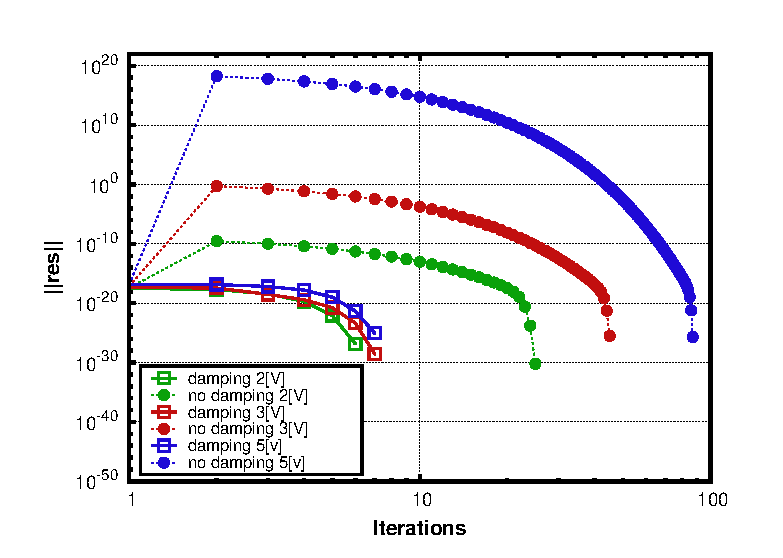
\includegraphics[height=7cm]{FiniteElementDiscretization/NLPconver/NLPconvergence.eps}}

\subfloat[][\emph{$t_k$ parameter.}\label{fig: Damping theta}]
{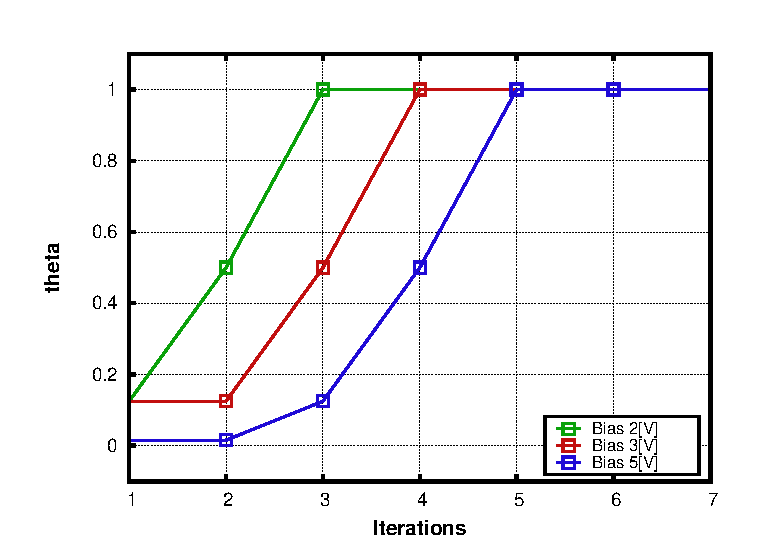
\includegraphics[height=7cm]{FiniteElementDiscretization/NLPconver/NLPtheta}}

\caption{(a) Number of iteration against residual for different voltages in a diode test case. (b) Magnitude of the damping parameter $t_k$.}

\end{figure}

\clearpage


\subsection{Continuity equations}
\label{sec: continuity equations}

Concerning with equation \referenzaeq{eq: system continuity equation} we can write the bilinear form as

\begin{equation}
\label{eq: weak formulation displacement}
a(u,v) =  \int_{\Omega_{Si}}  q D_n e^{\varphi^{i}/V_{th}} \nabla \psi_j \nabla \psi_i \, d\Omega + \int_{\Omega_{Si}} \sigma_n^{i-1} e^{\varphi^{i}/V_{th}} \psi_j \psi_i \, d\Omega.
\end{equation}

Even if this form allows an immediate analysis of well-posedness, the choice of using Slotboom variables $u_n$ and $u_p$ causes the onset of overflow problems due to the evaluation of $\exp(\varphi/V_{th})$, which can be a rapidly varying function according to the behaviour of the potential $\varphi$.

Therefore special care has to be taken in the treatment of the diffusion coefficient. In view of further discussion we introduce some useful notation. For each set $S \subset \Omega$ having measure $|S|$, we introduce the following averages of a given function $g$ that is integrable on $S$:

\begin{equation*}
\mathcal{M}_S(g) = \dfrac{\int_S g \, dS}{|S|}, \psp{15} \mathcal{H}_S = (\mathcal{M}_S(g^{-1}))^{-1} .
\end{equation*}

Notice that $\mathcal{M}_S$ is the usual integral average, while $\mathcal{H}_S$ is the \textit{harmonic average}. It is well-known that the use of the harmonic average provides a superior approximation performance in one spatial dimension \cite{BabuskaMixMet}.

The weak form \referenzaeq{eq: weak formulation displacement}  is the result of a standard displacement approach, although different variational formulations and therefore different finite element approximations may be used, like a primal mixed approach (PM).  First of all it is convenient to reformulate problem \referenzaeq{eq: LEC system new} by using relations \referenzaeq{eq: un slotboom} and \referenzaeq{eq: Jn slotboom} in a more generical form as:

\begin{equation}
\label{eq: LEC system slotboom generic}
\begin{cases}
\nabla \cdot \vect{J}_n(n)  +\sigma n = f & in \psp{3} \Omega_{Si}
 \\
 \vect{J}_n = qD_n e^{\varphi/V_{th}} \nabla (e^{-\varphi/V_{th}}n) & in \psp{3} \Omega_{Si}\\
n = n_D & on \psp{3} \Gamma_{D,Si}
 \\
 \vect{J}_n \cdot \vect{n} = 0 & on \psp{3} \Gamma_{N,Si}.
\end{cases}
\end{equation}

Problem \referenzaeq{eq: LEC system slotboom generic} can be discretized considering the \textit{Edge Averaged Finite Elements} (EAFE). The complete derivation of this scheme can be found in \cite{Zikatanov:EAFE1} \cite{Zikatanov:EAFE2}.

%We report here the weak formulation of \referenzaeq{eq: LEC system slotboom generic} which is well investigated in \cite{TesiDotDeFalco}, find $\vect{J}_n \in [L^2(\Omega)]^d$ and $n \in H^1_{\Gamma_{D,Si}}(\Omega)$ such that
%
%\begin{align}
%- \int_{\Omega_{Si}} \vect{J}_n\cdot \nabla v \, d\Omega + \int_{\Omega_{Si}} \sigma n v \, d\Omega = \int_{\Omega_{Si}} f v \, d\Omega \psp{10} \forall v \in H^1_{\Gamma_{D,Si}}(\Omega)
%\label{eq: weak form PM1} \\
%\int_{\Omega_{Si}} (qD_n e^{(\varphi/V_{th})})^{-1} \vect{J}_n\cdot \vect{q} \, d\Omega + \int_{\Omega_{Si}} \nabla(e^{(\varphi/V_{th})}n) \cdot \vect{q} \, d\Omega = 0 \psp{10} \forall \vect{q} \in [L^2(\Omega)]^d \label{eq: weak form PM2} 
%\end{align}
%
%In order to approximate $[L^2(\Omega)]^d$ we introduce a new discrete space
%
%\begin{equation}
%\Sigma_h := \left\{   \vect{q}_h \in  [L^2(\Omega)]^d : \vect{q}|_{K} \in [\mathbb{P}_0]^d \forall K \in \mathcal{T}_h\right\}
%\end{equation} 
%
%as usual $d$ is the dimension of $\Omega$ and if $d=3$, $\vect{q}_h$ is characterized for every $K \in \mathcal{T}_h$ by the triplet
%
%\begin{equation}
%\label{eq: form of qh}
%\vect{q}^h_{1,2,3} = \left\{ \begin{bmatrix} 1 \\ 0 \\ 0 \end{bmatrix}  \begin{bmatrix} 0 \\ 1 \\ 0 \end{bmatrix}  \begin{bmatrix} 0 \\ 0 \\ 1 \end{bmatrix}  \right\}
%\end{equation}
%
%Therefore \referenzaeq{eq: weak form PM1} and \referenzaeq{eq: weak form PM2} can restricted on a generic element $K$ and the related bilinear form reads
%
%\begin{equation}
%\label{eq: LEC discretized general}
%\left\{
%\begin{array}{rcl}
%a_h^K(n_h,v_h) & = & \int_{K}\vect{ J}_{n,h}^K(n_h) \nabla v_h \, dK + \int_{K} \sigma n_h v_h \, dK 
%\\
%\\
%F(v_h)^K & = & \int_K f v_h \, dK
%\\
%\\
%\vect{J}_{n,h}^K & = & D_K(qD_n e^{(\varphi/V_{th})}) \nabla  (e^{(-\varphi / V_{th})}n_h)
%\end{array}
%\right.
%\end{equation}
%
%where $D_K \in \mathbb{R}^{3\times 3}$ is the element stiffness matrix. Several treatments may be performed on this matrix
%
%\begin{equation}
%\label{eq: vari diffusion coeff}
% D_K(qD_n e^{(\varphi/V_{th})}) = 
% 	\begin{cases}
%		  \mathcal{M}_K(qD_n e^{(\varphi/V_{th})}) \\
%		  \mathcal{H}_K(qD_n e^{(\varphi/V_{th})}) \\
% 		  \dfrac{1}{|K|}\sum_{i=1}^6 \mathcal{H}_{e_i}(qD_ne^{(\varphi/V_{th})}) |e_i| s_i \vect{t}_i \vect{t}_i^T
% 		 \end{cases}
%\end{equation}
%
%
%These different approaches in the computation of the average of the diffusion coefficient are responsible for the quite different numerical perfomance of the relative methods.
%We already presented the standard average and the armonic average and we discussed briefly the advantages of them. 
%The latter equation in \referenzaeq{eq: vari diffusion coeff} introduces an exponentially treatment of the diffusion coefficient along each edge of the boundary $\partial K$ of the subdomain $K$. 
%
%Considering that along the edges the approximate flux density can be written as a function of its tangential components. We have for each edge $e_i$, the tangential component of $J_h^K(n_h)$
%
%\begin{align*}
%j_{e_i}  & =   \mathcal{H}_{e_i} \dfrac{\delta_i(e^{-\varphi /V_th}n_h)}{|e_i|} = \mathcal{H}_{e_i} \nabla (e^{-\varphi / V_{th}}n_h) \vect{t}_i \\
%& =  \mathcal{H}_{e_i}(qD_n e^{(\varphi/V_{th})}) \dfrac{\mathcal{B}(\delta_i(\varphi / V_{th}))n_{h,k} -  \mathcal{B}(-\delta_i(\varphi / V_{th}))n_{h,j}}{|e_i|}
%\end{align*}
%
%where 
%
%\begin{equation}
%\label{eq: peclet number}
%\delta_i(\varphi / V_{th}) = \dfrac{\varphi_k - \varphi_j}{V_{th}} = 2 \dfrac{(\vect{E}_K\cdot \vect{t}_{e_i}) |e_i|}{2\mathcal{H}_{e_i}(qD_n e^{(\varphi/V_{th})}) } = 2 \gamma_i
%\end{equation}
%
%\begin{equation}
%\mathcal{B}(z) = \left\{ \begin{array}{cl}
%\dfrac{z}{e^z-1} & z \neq 0
%\\
%1 & z = 0
%\end{array}
%\right.
%\end{equation}
%
%being $\vect{E}_K$ the relative electric field on $K$ and $|\gamma_i|$ the P\`eclet number associated with the edge $e_i$. 
%From \referenzaeq{eq: LEC discretized general} we immeditaly obtain:
%
%\begin{equation}
%\label{eq: exp fitted flux}
%\vect{J}_h^K = \dfrac{1}{|K|}\sum_{i=1}^6 |e_i| s_i j_{e_i} \vect{t}_i 
%\end{equation}
%
%Furthermore having defined the flux vector over $K$ in the form \referenzaeq{eq: exp fitted flux}, it is possible to construct a fimily of Galerkin finite element approximations for the continuity equations by a proper choice of the quantities $j_{e_i}$ (e.g. upwind techniques). 
%
%
%
%
%\subsubsection{The discretization scheme}
%
%Given the choice for $j_{e_i}$ and replacing the equation for $\vect{J}_h^K$ in the bilinear form \referenzaeq{eq: LEC discretized general}, we can compute the local system matrix as
%
%\begin{equation}
%\Phi_K  = 
%{
%\tiny 
%\left[
%\begin{array}{cccc}
%- \left( \begin{array}{c}
%a_{e12}\mathcal{B}_{12}L^K_{21} + \\
%a_{e13}\mathcal{B}_{13}L^K_{31} + \\
%a_{e14}\mathcal{B}_{14}L^K_{41}
%\end{array} \right)
%
%& a_{e12}\mathcal{B}_{12}L^K_{21} 
%& a_{e13}\mathcal{B}_{13}L^K_{31}
%& a_{e14}\mathcal{B}_{14}L^K_{41}
%\\
%
%%-----------------------------
%a_{e21}\mathcal{B}_{21}L^K_{12}
%&
%- \left( \begin{array}{c}
%a_{e21}\mathcal{B}_{21}L^K_{12} + \\
%a_{e23}\mathcal{B}_{23}L^K_{32} + \\
%a_{e24}\mathcal{B}_{24}L^K_{42}
%\end{array} \right)
%& a_{e23}\mathcal{B}_{12}L^K_{32}
%& a_{e24}\mathcal{B}_{12}L^K_{42}
%\\
%
%%-----------------------------
%a_{e31}\mathcal{B}_{31}L^K_{31}
%& a_{e31}\mathcal{B}_{32}L^K_{32}
%&
%- \left( \begin{array}{c}
%a_{e31}\mathcal{B}_{31}L^K_{31} + \\
%a_{e32}\mathcal{B}_{32}L^K_{32} + \\
%a_{e34}\mathcal{B}_{34}L^K_{34}
%\end{array} \right)
%
%&a_{e34}\mathcal{B}_{34}L^K_{34}
%\\
%
%%-----------------------------
%a_{e41}\mathcal{B}_{41}L^K_{41}
%& a_{e42}\mathcal{B}_{42}L^K_{42}
%&a_{e43}\mathcal{B}_{43}L^K_{43}
%&
%- \left( \begin{array}{c}
%a_{e41}\mathcal{B}_{41}L^K_{41} + \\
%a_{e42}\mathcal{B}_{42}L^K_{42} + \\
%a_{e43}\mathcal{B}_{43}L^K_{43}
%\end{array} \right)
%
%\end{array}
%\right]
%}
%\end{equation}
%
%\begin{equation}
%\label{eq: matrice continuità}
%A_K = \Phi_K + \dfrac{|K|}{4} diag (\sigma)
%\end{equation}
%
%\begin{equation}
%\vect{F}_K = \dfrac{|K|}{4} (f_1,f_2,f_3,f_4)^T
%\end{equation}
%
%denoting by  $\mathcal{B}_{ij}$ the Bernoulli function applied to the potential difference between node $j$ and node $i$.


The EAFE scheme is particularly suited for problems with a highly variable diffusion coefficient. Furthermore this approach has several good properties, i.e. in 2D simulation if $\mathcal{T}_h$ is a Delaunay partition the system matrix is an M-matrix \cite{BankMmatrixEAFE}. The main consequence of this statement is that the solution satisfying the \textit{Discrete Maximum Principle}. This is a notable property which implies that no negative concentrations are admitted. Unfortunately this property is not anymore valid in 3D framework, because the Delaunay condition on the mesh is not sufficient to guarantee that the system matrix is an M-matrix. A more general condition is presented in \cite{Zikatanov:EAFE1}.

\begin{Teorema}[Zikatanov condition]
The system matrix of the EAFE scheme is an M-matrix if and only if for any fixed edge E of the partition $\mathcal{T}_h$ the following inequality holds

\begin{equation}
\label{eq: mesh delaunay condition}
\omega_E = \dfrac{1}{d(d-1)} \sum_{K\supset E} |k_E^K|cot\theta_E^K \geq 0,
\end{equation}

where $\sum_{K \supset E}$ means summation over all simplexes $K$ containing $E$, $\theta_E^K$ is tha angle between the faces $f_i$, $f_j \in \mathcal{T}_h$ such that $f_i \bigcap f_j = E$  and $k_E^K$ is the edge in $K$ which does not share any verticies with $E$.
\end{Teorema}

\begin{Osservazione}
For $d=2$, condition \referenzaeq{eq: mesh delaunay condition} means that the sum of the angles opposite to any edge is less than or equal to $\pi$, which implies that the partition is a Delaunay triangulation.
\end{Osservazione}

\begin{Osservazione}
Condition \referenzaeq{eq: mesh delaunay condition} highlights that in order to satisfy the discrete maximum principle, a partition without obtuse angles is preferable.
\end{Osservazione}

We remark that presently meshing algorithm are oriented to care about the minimum angle of the elements, rather than the maximum, this implying that to obtain a mesh which satisfies condition \referenzaeq{eq: mesh delaunay condition} is a really difficult task. 

\figref{fig: cubo zikatanov} shows a simple partition of a cube performed with the Synopsis tool SNMESH. For every element we evaluated how many edges do not satisfy condition \referenzaeq{eq: mesh delaunay condition}.
It is clear that there are a lot of edges which do not fulfil the condition and a precise pattern cannot be signed out. When several bad edges belong to a single element we can identify the presence of many obtuse angles.

In order to avoid this problem some alternative solutions are proposed in the literature, like the \textit{Orthogonal Subdomain Collocation method} \cite{OSCputticorded}, but also this approach is not a definite solution. 

Therefore in presence of a negative concentration the most used technique in 3D numerical simulation is to local mesh refinement in the regions where trouble occurs, which often are the ones where the carrier density decreases.



\begin{figure}[!b]
\centering
{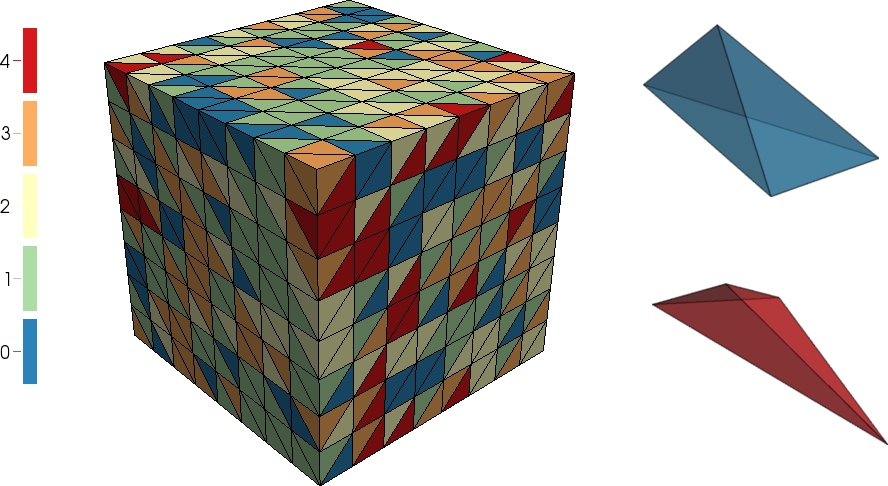
\includegraphics[width=0.75\textwidth , height = 5.5cm]{FiniteElementDiscretization/CuboElementi.png}}
\caption{Evaluation of the Zikatanov condition over a simple partition. Red elements do not satisfy condition  \referenzaeq{eq: mesh delaunay condition} over four edges while blue elements fully satisfy the criterion.}
\label{fig: cubo zikatanov}
\end{figure}

%\textcolor{red}{Vale la seguente uguaglianza?}
%\begin{equation}
%L_{ij} = s_{ij} \vect{t}_{ij} \cdot \nabla \psi_i
%\end{equation}
\clearpage
\chapter{Simulation results}
\label{chap: results}

In this chapter we present the work done in order to validate the numerical implementation of the discretization method illustrated in Chapter \ref{chap: finite element}, in the FEMOS 3D code compared with a reference simulation tool (SDEVICE, commercialized by Synopsis \cite{SdeviceManual}).
In particular we illustrate (and compare) the algorithm used to calculate the current at the ohmic contacts.

\section{Test cases}

We consider three kinds of semiconductor devices: 

\begin{itemize}
\setlength{\itemsep}{0.5pt}
\item {\bf p-n junction}
\item {\bf p-n junction in oxide}
\item {\bf n-channel / p-channel MOSFET}
\end{itemize}

\subsection{p-n junction}
\label{sec: PN}

In this example we consider a simple p-n junction. \figref{fig: diodo struttura} presents the partition and the doping profile for this test. The section of the parallelepiped is a $0.05 \times 0.05 [\mu m^2]$ square while the device is $0.1 [\mu m]$ long.  The number of vertices are $4933$, while the elements are $24576$.  The doping concentration is obtained setting a constant profile of acceptors over all the domain ($N_A^- = 1.0\times 10^{17} [cm^{-3}]$) overwhelmed by a doping profile of  donors ($N_D^+=1.0 \times 10^{18} [cm^{-3}]$) bounded on one side of the device and resulting in an almost abrupt junction. 
Two contacts are defined: (A) contact is placed at $Z=0.1[\mu m]$ and (B) contact is placed at $Z=0.0 [\mu m]$.  


\begin{figure}[!t]
\centering
\subfloat[][\emph{Mesh.}]
{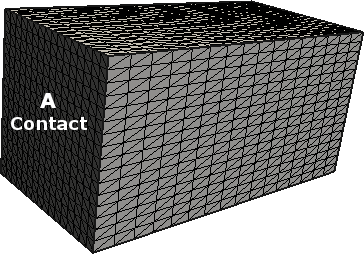
\includegraphics[width=0.35\textwidth , height=3.0cm]{Results/DIODE/AAA_structureandcontactFINITO.png}}
\hspace{0.06\textwidth}
\subfloat[][\emph{Doping concentration.}]
{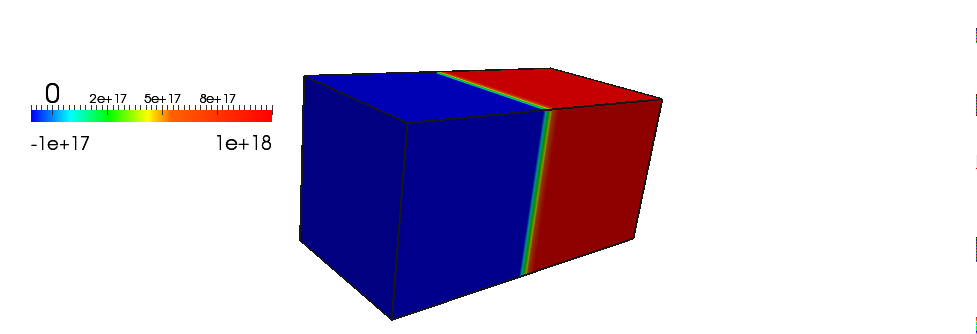
\includegraphics[width=0.35\textwidth ,  height=3.0cm]{Results/DIODE/AAA_Dopingconcentration.png}}
\hspace{0.04\textwidth}
{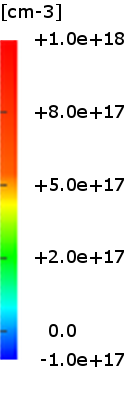
\includegraphics[width=0.1\textwidth ,  height=3.4cm]{Results/DIODE/LegendDopingDiode.png}}
\caption{p-n junction.}
\label{fig: diodo struttura}
\end{figure}


In order to analyze the operating function of the diode, two cases of direct bias are performed: $0.3[V]$-$1.0[V]$. The setting values and the parameters are summarized in \tabref{tab: diode direct}. 
\figref{fig: Solutions case test 0.3} reports the solutions for $V_A=0.3[V]$ and $V_A=1.0[V]$, along a line parallel to the Z-axis and placed at the center of the device. 
Because the built-in voltage is around $0.7 \div 0.8 [V]$ the behaviour of the device is different when the applied bias is below or above this threshold. 
At a bias voltage of $0.3[V]$, potential drop is almost bounded around the junction, and due to the asymmetric doping, is mostly extended in the p-side. Carriers cannot cross the potential barrier and this causes a low current flux inside the device.
At $1.0[V]$ the minority carrier density becomes almost ten order bigger, resulting in a large amount of current toward the contacts:  the device turns from exponential to linear resistive. This is clear in \figref{fig: diode 1v pot} where the potential shape becomes similar to a that of a resistance voltage profile (linear potential profile). Comparing the quasi Fermi potentials of \figref{fig: qf pot diode 03} and \figref{fig: qf pot diode 1} the boundary layers at contacts increase with the applied bias. This effect is related to the ohmic contact hypothesis, and can be avoided by adopting different boundary condition: this occurs also for the carrier concentration because at the contacts, charge neutrality and thermodynamic equilibrium  are imposed.

\figsref{fig: diode potential 03V}$\div$\ref{fig: pdensity 03V} shows the comparison between SDEVICE and FEMOS in 3D plots for electrostatic potential, electron and hole densities at $0.3[V]$, while \figsref{fig: diode potential 1V}$\div$\ref{fig: pdensity 1V} show the same comparison at $1.0[V]$. In both conditions the agreement is very good.

\begin{table}[!h]
\centering
\begin{tabular}{cccc}
\toprule
 Test case $[V]$  & Mobility model $[cm^2V^{-1}s^{-1}]$  & R/G model & $\epsilon_{Si}$\\
\midrule
$V_A=0.3$ & $\mu_n = 1417$, $\mu_p = 470.5$ & SRH, Auger & 11.6 \\
$V_A=1.0$ & $\mu_n = 1417$, $\mu_p = 470.5$ & SRH, Auger & 11.6 \\\bottomrule
\end{tabular}
\caption{p-n junction - list of settings, parameters and models.}
\label{tab: diode direct}
\end{table}


\begin{figure}[!h]
\centering

\subfloat[][\emph{Potential}]
{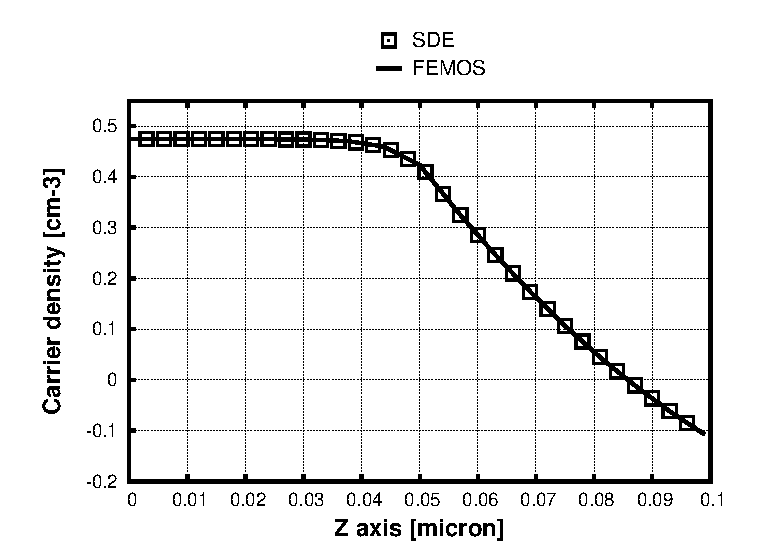
\includegraphics[width=0.5\textwidth , height=5cm]{DatiImmaginiTESI/Diode/PotentialZaxis03volt.eps}}
\subfloat[][\emph{Potential} \label{fig: diode 1v pot}]
{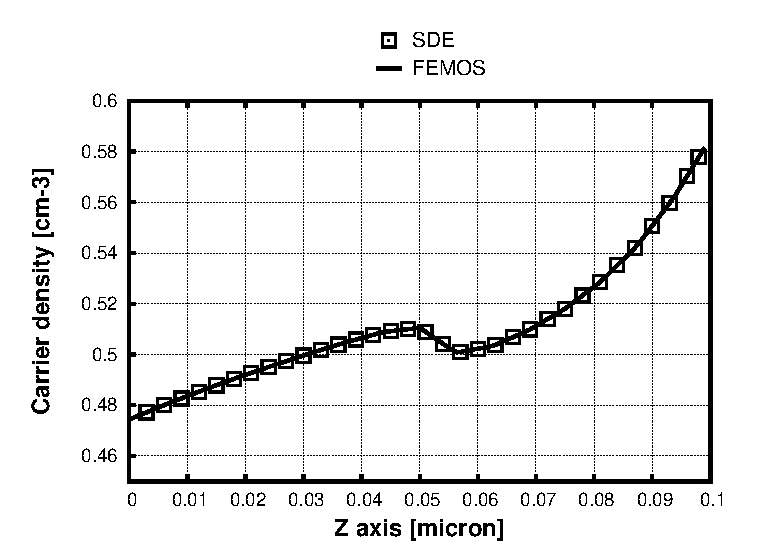
\includegraphics[width=0.5\textwidth , height=5cm]{DatiImmaginiTESI/Diode/PotentialZaxis1volt.eps}}


\subfloat[][\emph{Carriers}]
{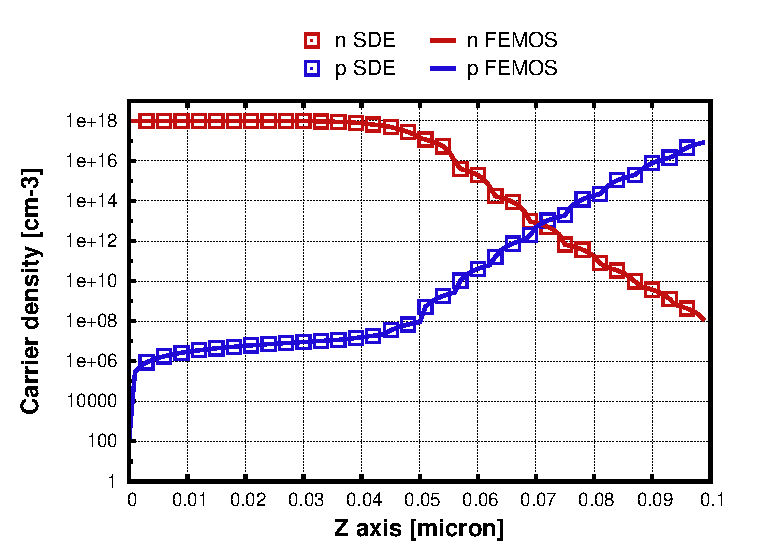
\includegraphics[width=0.5\textwidth , height=5cm]{DatiImmaginiTESI/Diode/DensitiesZaxis03volt.eps}}
\subfloat[][\emph{Carriers}]
{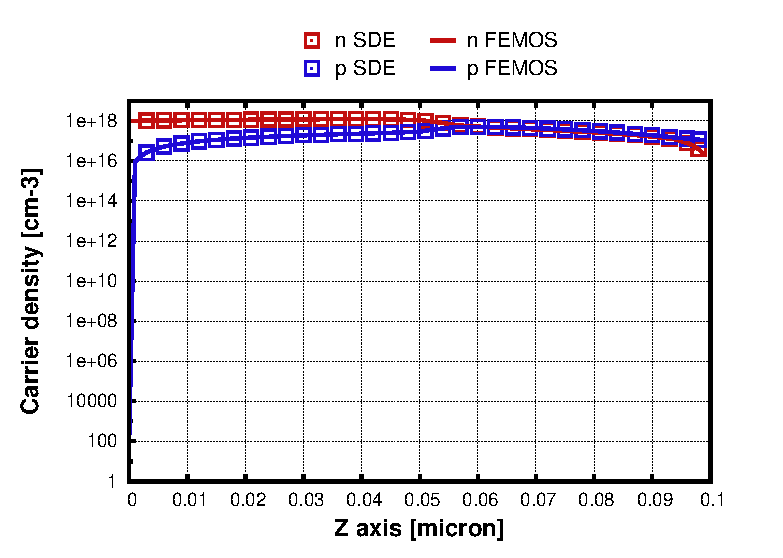
\includegraphics[width=0.5\textwidth , height=5cm]{DatiImmaginiTESI/Diode/DensitiesZaxis1volt.eps}}


\subfloat[][\emph{Quasi Fermi potentials} \label{fig: qf pot diode 03}]
{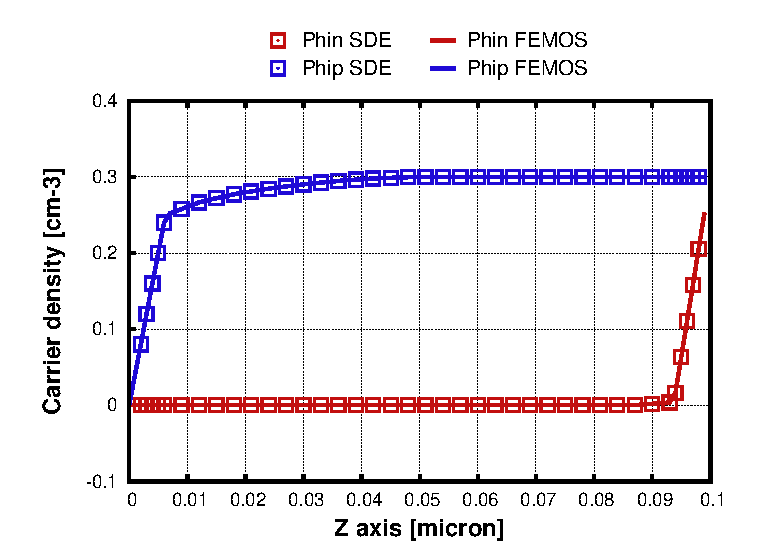
\includegraphics[width=0.5\textwidth , height=5cm]{DatiImmaginiTESI/Diode/QuasiFermiZaxis03volt.eps}}
\subfloat[][\emph{Quasi Fermi potentials} \label{fig: qf pot diode 1}]
{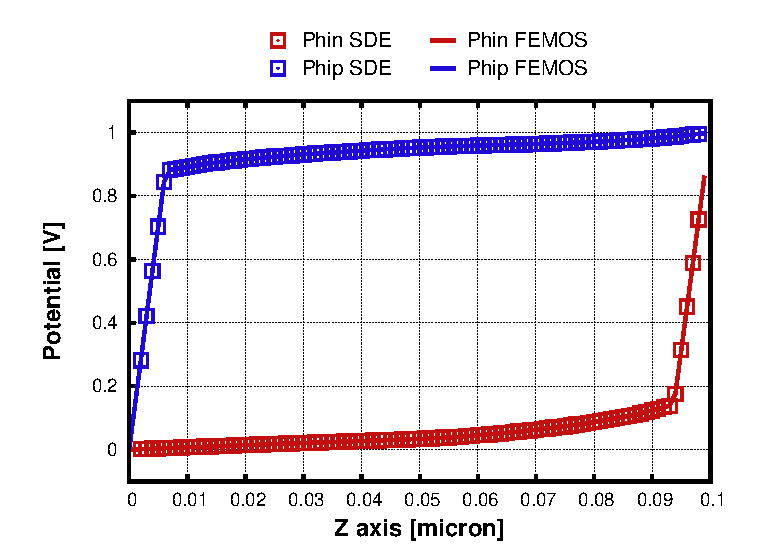
\includegraphics[width=0.5\textwidth , height=5cm]{DatiImmaginiTESI/Diode/QuasiFermiZaxis1volt.eps}}

\caption{1D plots of the solutions and the quasi fermi potential levels along the line parallel to the Z-axis and placed at the center of the device. On the left is presented the test case at $V_A=0.3[V]$ while on the right at $V_A=1.0[V]$.}
\label{fig: Solutions case test 0.3}
\end{figure}


\clearpage 

\begin{figure}[!h]
\centering
\subfloat[][\emph{FEMOS}]
{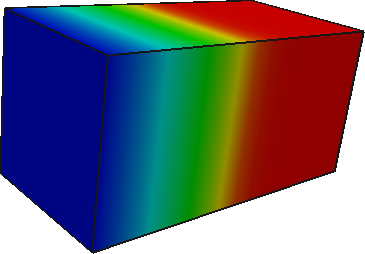
\includegraphics[width=0.38\textwidth , height=3.7cm]{Results/DIODE/FEMOS1817_potential03volt.png}}
\hspace{0.06\textwidth}
\subfloat[][\emph{SDEVICE}]
{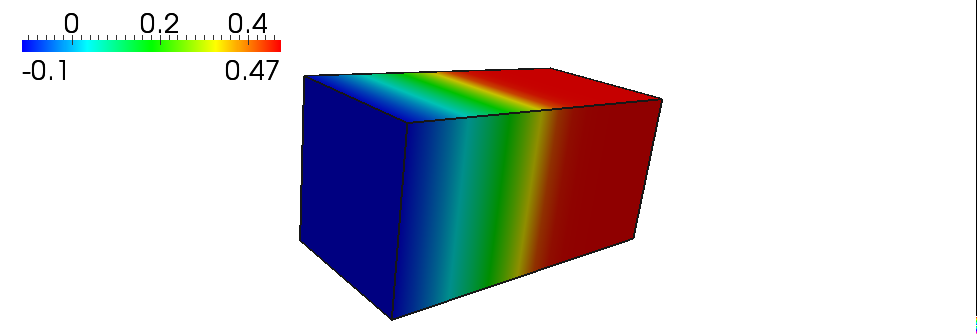
\includegraphics[width=0.38\textwidth , height=3.7cm]{Results/DIODE/SDEVICE1817_potential03volt.png}}
\hspace{0.04\textwidth}
{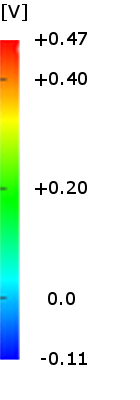
\includegraphics[width=0.1\textwidth , height=3.7cm]{Results/DIODE/LegendPotentialDiode03volt.png}}
\caption{p-n junction 0.3[V] - Electrostatic Potential.}
\label{fig: diode potential 03V}
\end{figure}


\vspace{1cm}

\begin{figure}[!h]
\centering
\subfloat[][\emph{FEMOS}]
{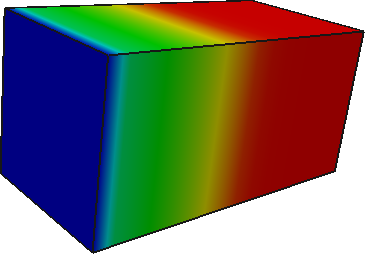
\includegraphics[width=0.38\textwidth , height=3.7cm]{Results/DIODE/FEMOS1817_edensity03volt.png}}
\hspace{0.06\textwidth}
\subfloat[][\emph{SDEVICE}]
{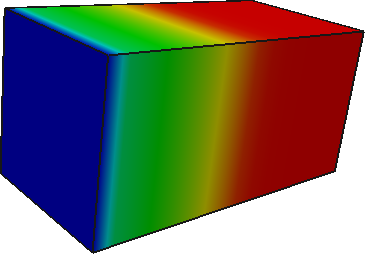
\includegraphics[width=0.38\textwidth , height=3.7cm]{Results/DIODE/FEMOS1817_edensity03volt.png}}
\hspace{0.04\textwidth}
{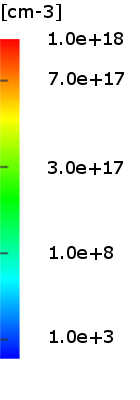
\includegraphics[width=0.1\textwidth , height=3.7cm]{Results/DIODE/LegendEdensityDiode03volt.png}}
\caption{p-n junction 0.3[V] -  Electron density.}
\label{fig: ndensity 03V}
\end{figure}

\vspace{1cm}

\begin{figure}[!h]
\centering
\subfloat[][\emph{FEMOS}]
{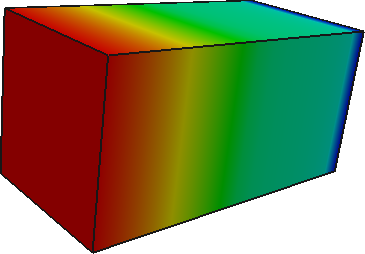
\includegraphics[width=0.38\textwidth , height=3.7cm]{Results/DIODE/FEMOS1817_hdensity03volt.png}}
\hspace{0.06\textwidth}
\subfloat[][\emph{SDEVICE}]
{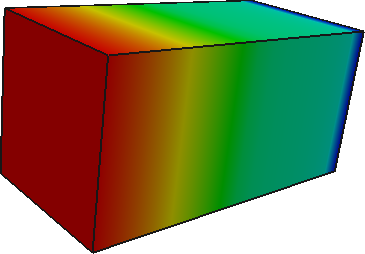
\includegraphics[width=0.38\textwidth , height=3.7cm]{Results/DIODE/FEMOS1817_hdensity03volt.png}}
\hspace{0.04\textwidth}
{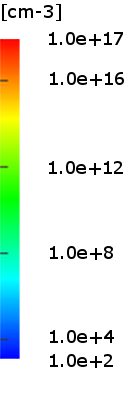
\includegraphics[width=0.1\textwidth , height=3.7cm]{Results/DIODE/LegendHdensityDiode03volt.png}}
\caption{p-n junction 0.3[V] - Hole density.}
\label{fig: pdensity 03V}
\end{figure}


\clearpage

\begin{figure}[!h]
\centering
\subfloat[][\emph{FEMOS}]
{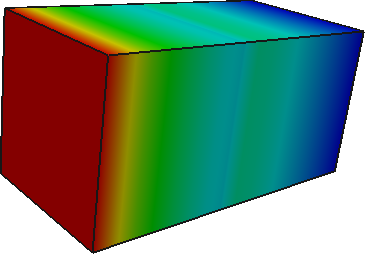
\includegraphics[width=0.38\textwidth , height=3.7cm]{Results/DIODE/FEMOS1817_potential1voltONLYDEVICE.png}}
\hspace{0.06\textwidth}
\subfloat[][\emph{SDEVICE}]
{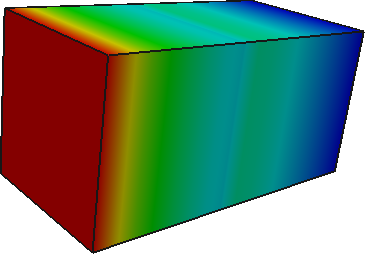
\includegraphics[width=0.38\textwidth , height=3.7cm]{Results/DIODE/FEMOS1817_potential1voltONLYDEVICE.png}}
\hspace{0.04\textwidth}
{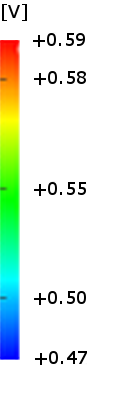
\includegraphics[width=0.1\textwidth , height=3.7cm]{Results/DIODE/LegendPotentialDiode1volt.png}}
\caption{p-n junction 1.0[V] - Electrostatic Potential.}
\label{fig: diode potential 1V}
\end{figure}

\vspace{1cm}

\begin{figure}[!h]
\centering
\subfloat[][\emph{FEMOS}]
{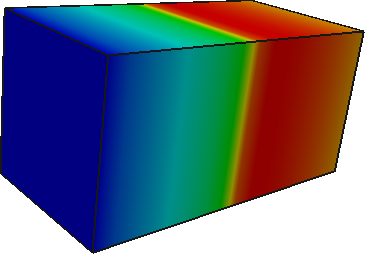
\includegraphics[width=0.38\textwidth , height=3.7cm]{Results/DIODE/FEMOS1817_edensity1voltLINEARONLYDEVICE.png}}
\hspace{0.06\textwidth}
\subfloat[][\emph{SDEVICE}]
{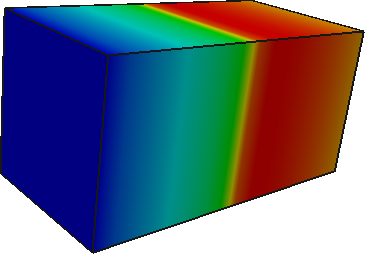
\includegraphics[width=0.38\textwidth , height=3.7cm]{Results/DIODE/FEMOS1817_edensity1voltLINEARONLYDEVICE.png}}
\hspace{0.04\textwidth}
{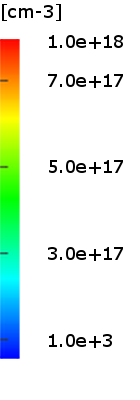
\includegraphics[width=0.1\textwidth , height=3.7cm]{Results/DIODE/LegendEdensityDiode1volt.png}}
\caption{p-n junction 1.0[V] -  Electron density.}
\label{fig: ndensity 1V}
\end{figure}

\vspace{1cm}

\begin{figure}[!h]
\centering
\subfloat[][\emph{FEMOS}]
{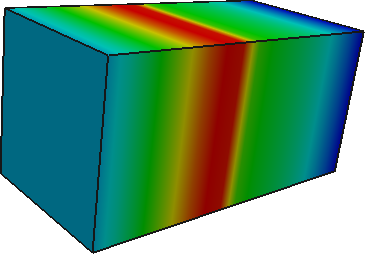
\includegraphics[width=0.38\textwidth , height=3.7cm]{Results/DIODE/FEMOS1817_hdensity1voltLINEARONLYDEVICE.png}}
\hspace{0.06\textwidth}
\subfloat[][\emph{SDEVICE}]
{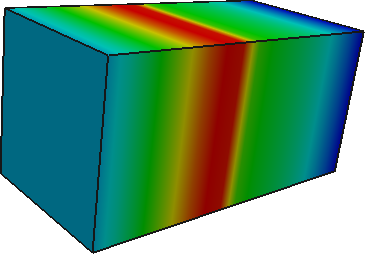
\includegraphics[width=0.38\textwidth , height=3.7cm]{Results/DIODE/FEMOS1817_hdensity1voltLINEARONLYDEVICE.png}}
\hspace{0.04\textwidth}
{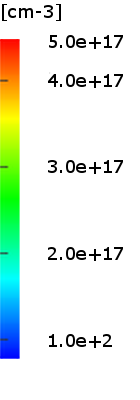
\includegraphics[width=0.1\textwidth , height=3.7cm]{Results/DIODE/LegendHdensityDiode1volt.png}}
\caption{p-n junction 1.0[V] - Hole density.}
\label{fig: pdensity 1V}
\end{figure}

\clearpage

\subsubsection{Computational cost and initial condition}

Computational experience demonstrates that convergence of the Gummel algorithm is strictly related to the kind of chosen initial condition: the closest to solution, the better the convergence. However, to predict in every situation the possible shape of the solutions is hard (if not even impossible). For this reason we have adopted a common and general approach splitting the domain in several regions according to their doping concentration: each of the semiconductor regions are treated as they are in equilibrium with the nearest contact, then the initial guess for $\varphi$ is obtained using the relations \referenzaeq{eq: non eq n density mb} or \referenzaeq{eq: non eq p density mb}. This choice corresponds to a case close to equilibrium and guarantees good performance of the algorithm.

In order to analyze the response of the system at different bias an additional test is realized: in the range between $0.0[V]$ and $3.0[V]$ several voltages are applied on the previous device and for each bias point the initial guess is computed as described.

\figref{fig: tempi computazionali 1} shows how the computational cost increases as the applied bias is increased. Moreover as expected if the mesh is finer, the time needed to find the solution increases, resulting in a rigid upper shift of the curve.


\begin{figure}[!b]
\centering
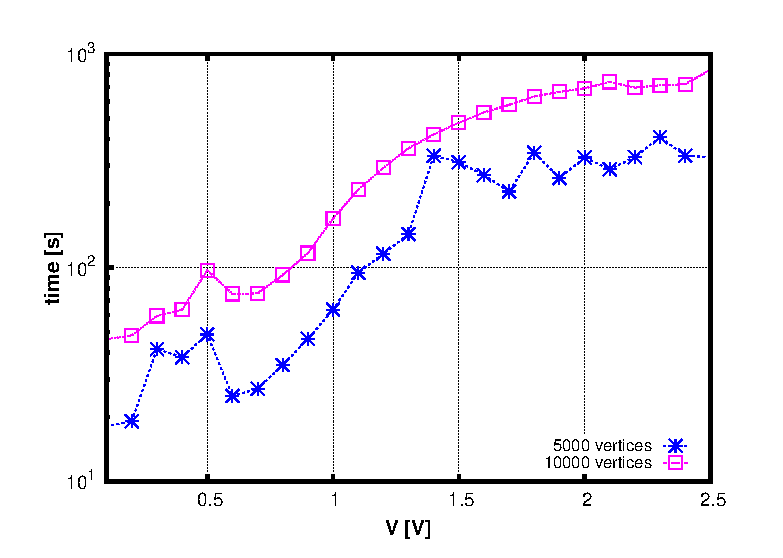
\includegraphics[height=7cm]
{Results/Caratteristiche/Diode/ComputationalTimeDifferentMeshes.eps}
\caption{Total time Gummel Map.}
 \label{fig: tempi computazionali 1}
 \end{figure}
 
 Let us consider the case with a coarse mesh. In \figref{fig: tempi computazionali 2} it is clear how the average time spent to solve the NLP and the DD equations remains almost unchanged. On the contrary the number of GM iterations needed by the system to reach the solution, increases for voltages above $\approx 1.5[V]$.

A possible explanation of this trend can be found comparing solution and initial guess for a bias below and above $1.5[V]$ (similar considerations may be done for carrier densities). When voltage is low, like in \figref{fig: different biast initial step 1} ($V_A = 0.1[V]$), the potential shape is well predicted by the initial guess, resulting in a better convergence for the Gummel map algorithm. On the contrary in \figref{fig: different biast initial step 2} ($V_A=1.6[V]$) the device operates as a resistence and the potential profile is close to a linear function: this implies that the solution is far from the initial guess as equilibrium condition and the algorithm needs more steps.


 
 \begin{figure}[!t]
\centering
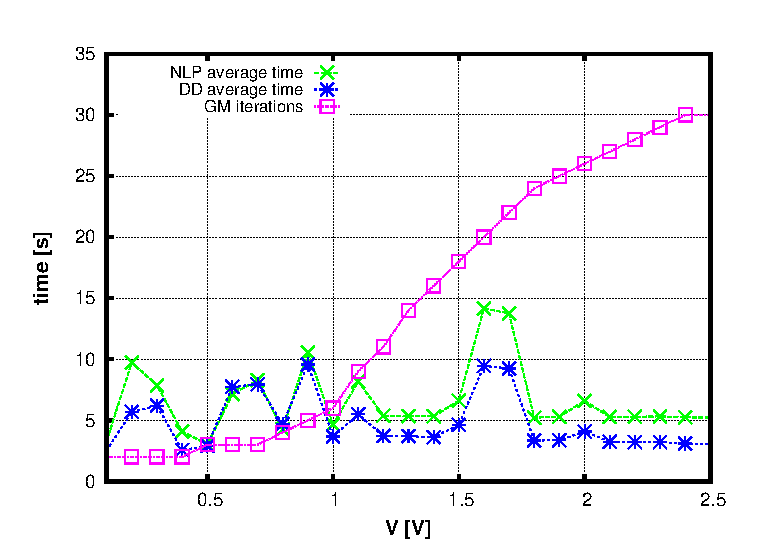
\includegraphics[height=7cm]{Results/Caratteristiche/Diode/ConfrontoTempiNLPDDGMiterations.eps}
\caption{Time to solve the NLP and DD equations, and number of  iterations of the Gummel map.}
\label{fig: tempi computazionali 2}
\end{figure}

\begin{figure}[!b]
\centering
\subfloat[][\label{fig: different biast initial step 1}]
{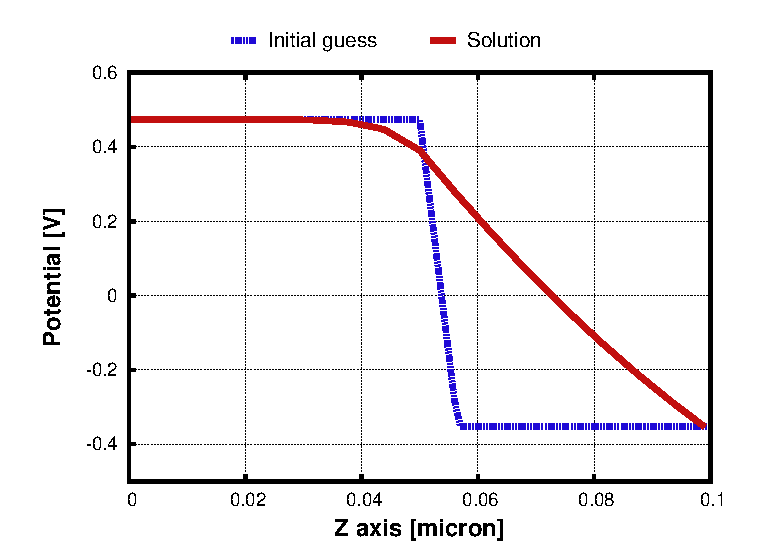
\includegraphics[height=4.5cm]{DatiImmaginiTESI/Diode/PotentialZaxis01volt.eps}}
\subfloat[][\label{fig: different biast initial step 2}]
{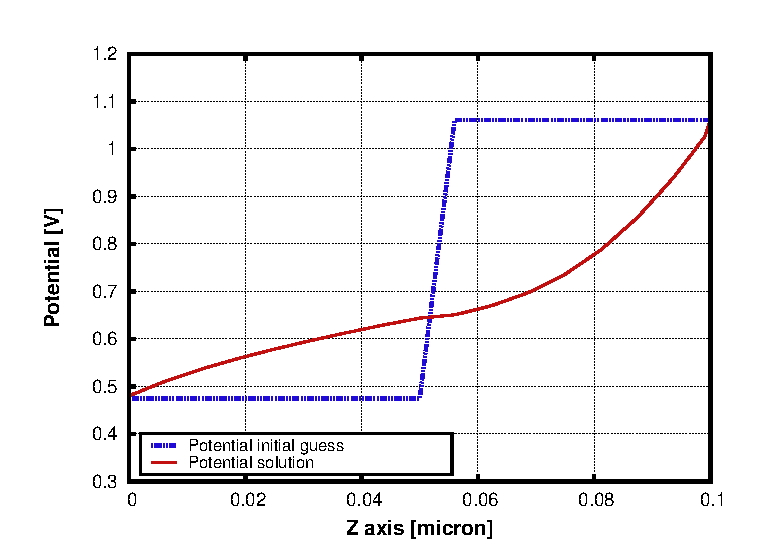
\includegraphics[height=4.5cm]{DatiImmaginiTESI/Diode/PotentialZaxis15volt.eps}}
\caption{Initial guess for different bias compared with the final solution.}
\label{fig: different biast initial step}
\end{figure}
 



\clearpage


\subsection{p-n junction in oxide}
\label{sec: PNOX}

In this test case a silicon p-n junction $0.3[\mu m]$ long is surrounded by an oxide layer $0.025[\mu m]$ thick. The section of the silicon part is a $0.1 \times 0.1 [\mu m^2]$ square.  We employ $6334$ vertices and $33121$ elements overall the domain. The structure and the doping are shown in \figref{fig: structure diodeox}. The setting of the electrodes is similar to the previous test case and contacts are defined only on silicon surface. 
\tabref{tab: diodeox 3d} reports settings, models and parameters used in the simulations.

\figref{fig: plot 1D diodeox} shows the solutions and the quasi Fermi potential levels along a line parallel to the Z-axis and placed at the center of the device. The main features are similar to the previous test case, also for the boundary layers at contact in carriers and quasi Fermi potentials.
\figsref{fig: potential diodeox} $\div$ \ref{fig: hdensity diodeox} show the 3D solutions for the test at $0.3[V]$, while \figref{fig: potential diodeox 1V}$\div$\ref{fig: hdensity diodeox 1V} refer to the case at $1.0[V]$. Both the 1D cuts and 3D plots agreement with the commercial software is very good. 

\vspace{0.5cm}

\begin{figure}[!h]
\centering
\subfloat[][\emph{Mesh}]
{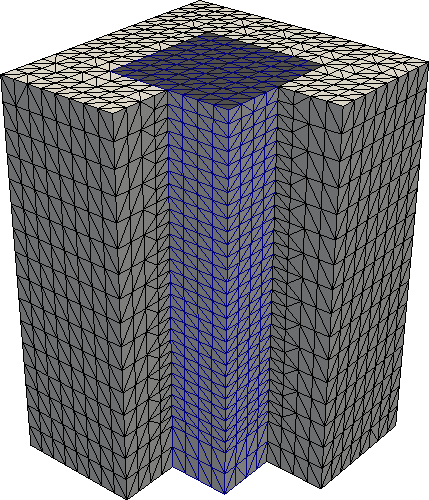
\includegraphics[width=0.33\textwidth , height=5cm]{Results/DIODEOX/AAA_structureandcontact2.png}}
\hspace{0.06\textwidth}
\subfloat[][\emph{Doping concentration}]
{\includegraphics[width=0.33\textwidth ,height=5cm]{Results/DIODEOX/AAA_Dopingconcentration2.png}}
\hspace{0.04\textwidth}
{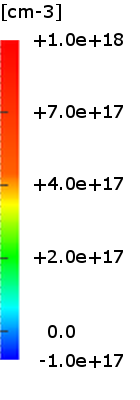
\includegraphics[width=0.1\textwidth ,height=4.5cm]{Results/DIODEOX/LegendDopingDiodeOx.png}}
\caption{Test case p-n junction in oxide.}
\label{fig: structure diodeox}
\end{figure}


\vspace{0.5cm}

\begin{table}[!h]
\centering
\begin{tabular}{ccccc}
\toprule
 Test case  & Mobility model & \multirow{2}*{R/G model} & \multirow{2}*{$\epsilon_{Si}$} & \multirow{2}*{$\epsilon_{0x}$}  \\
 $[V]$ & $[cm^2V^{-1}s^{-1}]$ & & & \\
\midrule
$V_A=0.3$ & $\mu_n = 1417$, $\mu_p = 470.5$ & SRH, Auger & 11.6 & 3.9 \\
$V_A=1.0$ & $\mu_n = 1417$, $\mu_p = 470.5$ & SRH, Auger & 11.6 & 3.9 \\\bottomrule
\end{tabular}
\caption{p-n junction in oxide - list of settings, parameters and models.}
\label{tab: diodeox 3d}
\end{table}




\begin{figure}[!t]
\centering

\subfloat[][\emph{Electrostatic potential.}]
{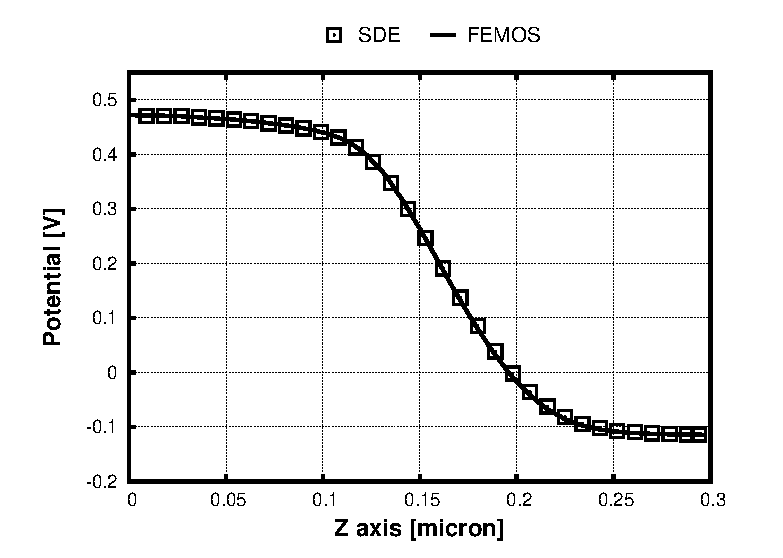
\includegraphics[width=0.5\textwidth , height=5cm]{DatiImmaginiTESI/DiodeOx/PotentialZaxis.eps}}
\subfloat[][\emph{Electrostatic potential.}]
{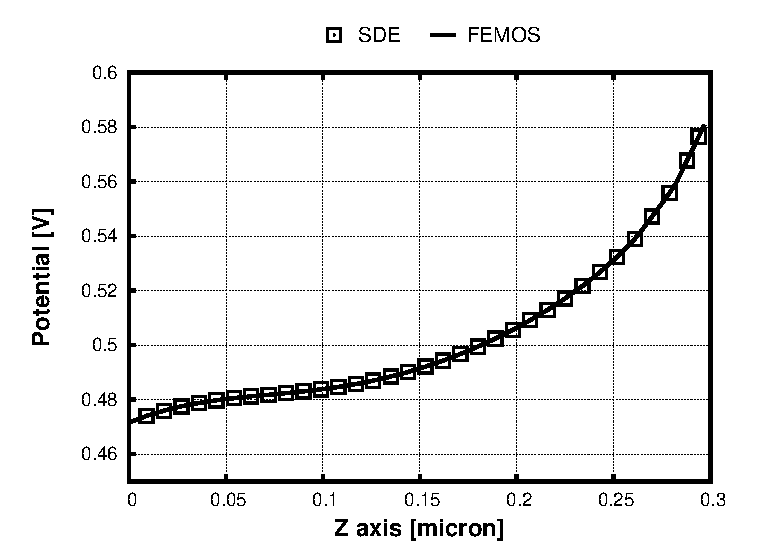
\includegraphics[width=0.5\textwidth , height=5cm]{DatiImmaginiTESI/DiodeOx/PotentialZaxis1VOLT.eps}}


\subfloat[][\emph{Hole and electron densities.}]
{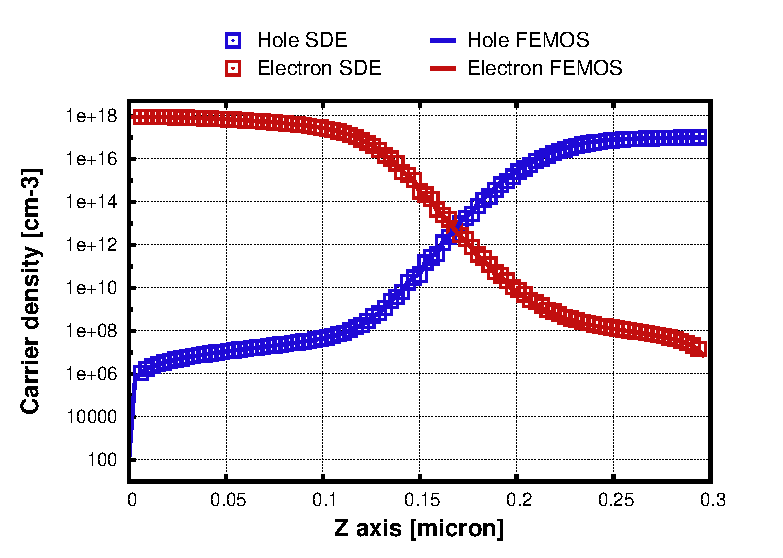
\includegraphics[width=0.5\textwidth , height=5cm]{DatiImmaginiTESI/DiodeOx/DensityZaxis.eps}}
\subfloat[][\emph{Hole and electron densities.}]
{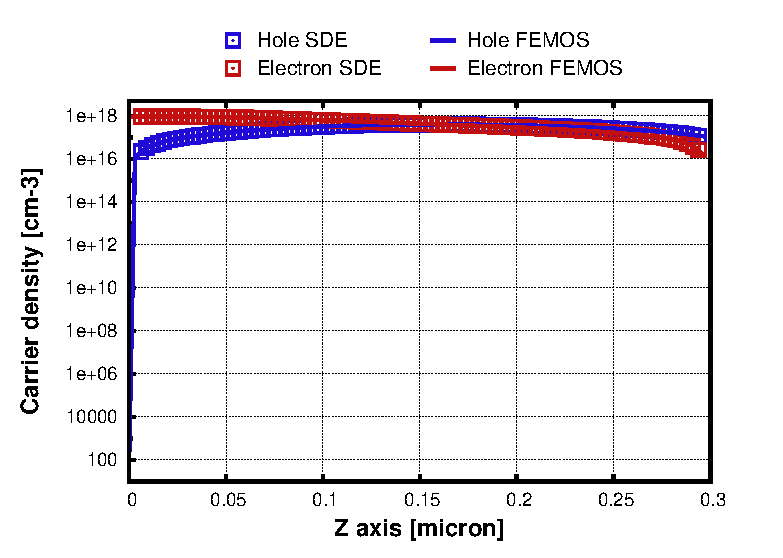
\includegraphics[width=0.5\textwidth , height=5cm]{DatiImmaginiTESI/DiodeOx/DensityZaxis1VOLT.eps}}


\subfloat[][\emph{Quasi Fermi potential levels.}]
{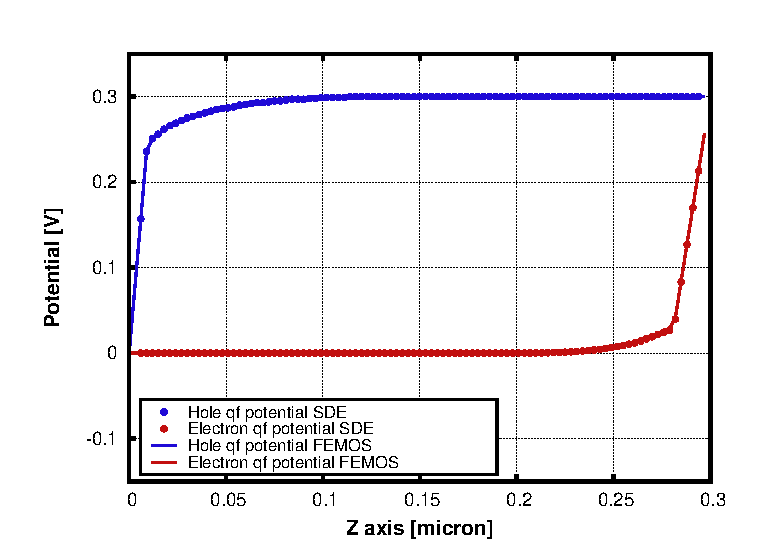
\includegraphics[width=0.5\textwidth , height=5cm]{DatiImmaginiTESI/DiodeOx/QFPotentialZaxis.eps}}
\subfloat[][\emph{Quasi Fermi potential levels.}]
{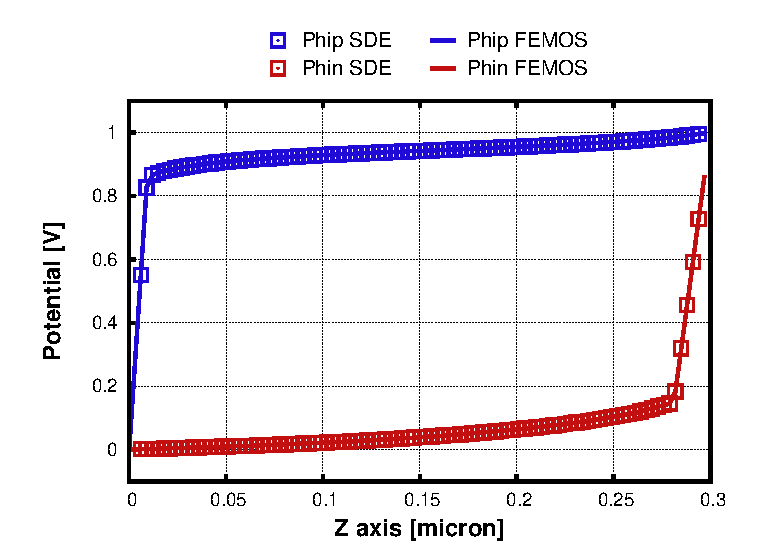
\includegraphics[width=0.5\textwidth , height=5cm]{DatiImmaginiTESI/DiodeOx/QFPotentialZaxis1VOLT.eps}}


\caption{1D plots of the solutions and the quasi Fermi potential levels along the line parallel to the Z-axis and placed at the center of the device. On the left test case at $V_A=0.3[V]$ is reported while on the right at $V_A=1.0[V]$.}
\label{fig: plot 1D diodeox}
\end{figure}

\clearpage


\begin{figure}[!h]
\centering
\subfloat[][\emph{FEMOS}]
{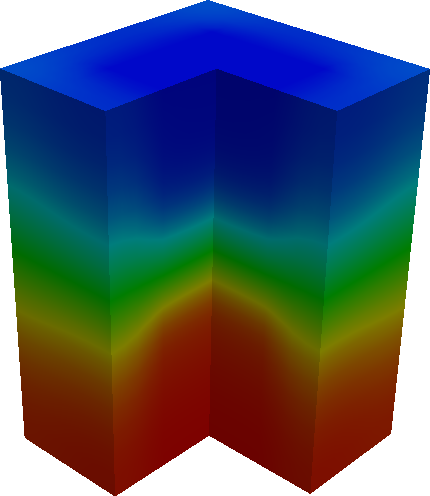
\includegraphics[width=0.3\textwidth ,height=4.5cm]{Results/DIODEOX/FEMOS1817_potential03volt.png}}
\hspace{0.1\textwidth}
\subfloat[][\emph{SDEVICE}]
{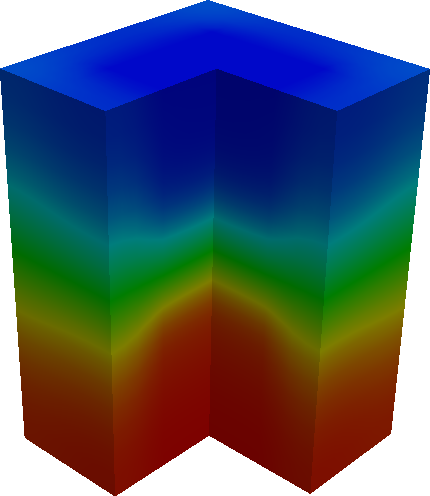
\includegraphics[width=0.3\textwidth ,height=4.5cm]{Results/DIODEOX/FEMOS1817_potential03volt.png}}
\hspace{0.04\textwidth}
{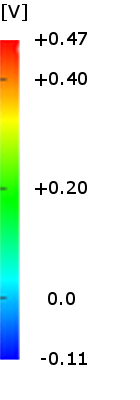
\includegraphics[width=0.1\textwidth ,height=4.5cm]{Results/DIODE/LegendPotentialDiode03volt.png}}
\caption{p-n junction in oxide 0.3[V] - ElectrostaticPotential.}
\label{fig: potential diodeox}
\end{figure}

\vspace{0.5cm}

\begin{figure}[!h]
\centering
\subfloat[][\emph{FEMOS}]
{\includegraphics[width=0.3\textwidth ,height=4.5cm]{Results/DIODEOX/FEMOS1817_edensity03volt.png}}
\hspace{0.1\textwidth}
\subfloat[][\emph{SDEVICE}]
{\includegraphics[width=0.3\textwidth ,height=4.5cm]{Results/DIODEOX/FEMOS1817_edensity03volt.png}}
\hspace{0.04\textwidth}
{\includegraphics[width=0.1\textwidth ,height=4.5cm]{Results/DIODEOX/LegendEdensityDiodeOx03volt.png}}
\caption{p-n junction in oxide 0.3[V] - Electron density.}
\label{fig: edensity diodeox}
\end{figure}

\vspace{0.5cm}

\begin{figure}[!h]
\centering
\subfloat[][\emph{FEMOS}]
{\includegraphics[width=0.3\textwidth ,height=4.5cm]{Results/DIODEOX/FEMOS1817_hdensity03volt.png}}
\hspace{0.1\textwidth}
\subfloat[][\emph{SDEVICE}]
{\includegraphics[width=0.3\textwidth ,height=4.5cm]{Results/DIODEOX/FEMOS1817_hdensity03volt.png}}
\hspace{0.04\textwidth}
{\includegraphics[width=0.1\textwidth ,height=4.5cm]{Results/DIODEOX/LegendHdensityDiodeOx03volt.png}}
\caption{p-n junction in oxide 0.3[V] - Hole density.}
\label{fig: hdensity diodeox}
\end{figure}

\clearpage


\begin{figure}[!h]
\centering
\subfloat[][\emph{FEMOS}]
{\includegraphics[width=0.3\textwidth ,height=4.5cm]{Results/DIODEOX/FEMOS1817_potential1voltONLYDEVICE.png}}
\hspace{0.1\textwidth}
\subfloat[][\emph{SDEVICE}]
{\includegraphics[width=0.3\textwidth ,height=4.5cm]{Results/DIODEOX/FEMOS1817_potential1voltONLYDEVICE.png}}
\hspace{0.04\textwidth}
{\includegraphics[width=0.1\textwidth ,height=4.5cm]{Results/DIODE/LegendPotentialDiode1volt.png}}
\caption{p-n junction in oxide 1.0[V] - Electrostatic Potential.}
\label{fig: potential diodeox 1V}
\end{figure}

\vspace{0.5cm}

\begin{figure}[!h]
\centering
\subfloat[][\emph{FEMOS}]
{\includegraphics[width=0.3\textwidth ,height=4.5cm]{Results/DIODEOX/EdensityLINEARDIODEOXONLYDEVICE.png}}
\hspace{0.1\textwidth}
\subfloat[][\emph{SDEVICE}]
{\includegraphics[width=0.3\textwidth ,height=4.5cm]{Results/DIODEOX/EdensityLINEARDIODEOXONLYDEVICE.png}}
\hspace{0.04\textwidth}
{\includegraphics[width=0.1\textwidth ,height=4.5cm]{Results/DIODEOX/LegendEdensityDiodeOx1volt.png}}
\caption{p-n junction in oxide 1.0[V] - Electron density.}
\label{fig: edensity diodeox 1V}
\end{figure}

\vspace{0.5cm}

\begin{figure}[!h]
\centering
\subfloat[][\emph{FEMOS}]
{\includegraphics[width=0.3\textwidth ,height=4.5cm]{Results/DIODEOX/HdensityLINEARDIODEOXONLYDEVICE.png}}
\hspace{0.1\textwidth}
\subfloat[][\emph{SDEVICE}]
{\includegraphics[width=0.3\textwidth ,height=4.5cm]{Results/DIODEOX/HdensityLINEARDIODEOXONLYDEVICE.png}}
\hspace{0.04\textwidth}
{\includegraphics[width=0.1\textwidth ,height=4.5cm]{Results/DIODEOX/LegendHdensityDiodeOx1volt.png}}
\caption{p-n junction in oxide 1.0[V] - Hole density.}
\label{fig: hdensity diodeox 1V}
\end{figure}

\clearpage





\subsubsection{3D effect on the electric field}


\figref{fig: potential diodeox} shows how at low bias the electrostatic potential behaves in a different manner in the oxide with the respect to the silicon region.
Since we impose $\nabla \varphi \cdot \vect{n}=0$ on the oxide boundary no field lines of the electric field can cross that boundary and as a consequence field lines can start and end only at contact A or B.
The electric field inside the device is due only to the displacement effect in the junction of the silicon which imposes the electric response also in the oxide material where the solution is no more linear. \figref{fig: electric field diode} reports the electric field lines in the case $V_A=0.3[V]$ compared with the commercial software. The lower magnitude of the electric field in the oxide, results in a more diffused potential.

At high bias (\figref{fig: potential diodeox 1V}) the influence of the contacts (A,B) becomes higher and the electrostatic potential is much more similiar in the two subdomains.


\vspace{1cm}

\begin{figure}[!h]
\centering
\subfloat[][\emph{FEMOS}]
{\includegraphics[width=0.38\textwidth ,height=5.5cm]{Results/DIODEOX/FEMOS1817_electricfield03volt.png}}
\hspace{0.05\textwidth}
\subfloat[][\emph{SDEVICE}]
{\includegraphics[width=0.38\textwidth ,height=5.5cm]{Results/DIODEOX/SDEVICE1817_electricfield03volt.png}}
\hspace{0.04\textwidth}
{\includegraphics[width=0.1\textwidth ,height=5cm]{Results/DIODEOX/LegendElectricFieldDiodeOx03volt.png}}
\caption{Test case dide p-n in oxide 0.3[V] - Electric field.}
\label{fig: electric field diode}
\end{figure}

\vspace{0.5cm}


It is important to notice that the displacement formulation approach does not satisfied  in a strong manner the princinple of action and reaction at \textcolor{red}{?} boundaries.
This is equivalent to saying that given two elements $K_i,K_j\in \mathcal{T}_h$ such that $K_i \bigcap K_j = f_i$ where $f_i \in \mathcal{F}_h$ and denoting by $\vect{n}_{i}$ the outward normal vector of $\partial K_i$ and $\vect{n}_{j}$ the outward normal vector of $\partial K_j$,  the following equations are satisfied only in a weak sense:

\begin{align}
\vect{D}|_{K_i}\cdot \vect{n}_{i} & = \vect{D}|_{K_j} \cdot \vect{n}_{j} \label{eq: conservazione vettore spostamento}\\
\vect{J}_n|_{K_i}\cdot \vect{n}_{i} & = \vect{J}_n|_{K_j}\cdot \vect{n}_{j} \\
\vect{J}_p|_{K_i}\cdot \vect{n}_{i} & = \vect{J}_p|_{K_j}\cdot \vect{n}_{j} .
\end{align}


In fact, taking in consideration equation \referenzaeq{eq: conservazione vettore spostamento}, we can state that along the interface silicon-oxide the following equality holds

\begin{equation}
\label{eq: rapporto campi}
\epsilon_{ox}\vect{E}|_{K_i}\cdot \vect{n}_{i} = \epsilon_{Si}\vect{E}|_{K_j} \cdot \vect{n}_{j} \psp{5} \Rightarrow \psp{5}  [\vect{E}|_{K_i}]_y = \dfrac{\epsilon_{Si}}{\epsilon_{ox}}[\vect{E}|_{K_j}]_y.
\end{equation}  

According with the parameters used in the simulations the jump of the electric field component from oxide to semiconductor is around $3.00$. \figref{fig: salto electric field} shows the plots of $E_y$ along a line parallel to the Y-axis crossing both oxide and silicon: the ratio expressed by \referenzaeq{eq: rapporto campi} is almost $3.6$ at $y=0.05[\mu m]$ and $y = 0.15[\mu m]$ where the interfaces are located.

Each tetrahedral interface of the partition is affected by this problem, which means that the normal component of the electric field from one element of the grid to the neighbouring is not conserved even if the material is homogeneous and there is no charge at the interface. Despite this drawback, the solutions are acceptable. But if we would satisfy equation \referenzaeq{eq: conservazione vettore spostamento} in a strong manner, the use of a mixed-hybrid formulation is needed which ensures the conservation of the flux also under possbile strong discontinuities of material properties.


\begin{figure}[!h]
\centering
\includegraphics[height=5cm]{DatiImmaginiTESI/DiodeOx/ElectricFieldYaxis.eps}
\caption{$E_y$ along a line parallel to Y-axis, $z=0.22[\mu m]$ and $x=0.1[\mu m]$.}
\label{fig: salto electric field}
\end{figure}


\clearpage





\subsection{n-channel MOSFET}
\label{sec: MOS}

The description of functioning of a MOSFET device can be found in \cite{ModernVLSIdevices}: it is a four-terminal device with the electrodes designated as gate (G), source (S), drain (D) and substrate or bulk (B). The gate electrode is usually made of metal or heavily doped polysilicon and is separated from the substrate by a thin silicon dioxide. The surface region under the gate oxide between source and drain is called \textit{channel} region.
Because the current in a MOSFET is due by carriers of one polarity, the MOSFET is usually referred as a unipolar or majority-carrier device: n-channel (n-MOSFET) and p-channel (p-MOSFET) are considered in the test. A \textit{n-MOSFET} (p-MOSFET) consists of a p-type (n-type) silicon substrate into which two n-regions (p-regions) are designed as source and drain. The n-regions (p-regions) are doped according with a Gaussian profile as in a real implantation process. 
\figref{fig: mos geometry 1} and \figref{fig: mos geometry 2} show the geometry and the doping concentration for the n-MOSFET with a coarse mesh ($2739$ vertices and $12338$ elements). 
We note that the mesh has been refined where the more interesting phenomena occur, i.e., along channel and at drain/source contacts.

If a sufficiently large positive voltage is applied to the gate, the silicon surface is inverted to n-type (p-type), which forms a conducting channel between the source and drain: applying a small positive voltage to the drain (source) the electrons (holes) start to flow from source (drain) to drain (source) and therefore a current is generated. 

\begin{figure}[!b]
\centering
\subfloat[][\emph{Mesh}\label{fig: mos geometry 1}]
{\includegraphics[width=0.38\textwidth ,height=4.3cm]
{Results/MOS/AAA_MeshAndContact.png}}
\hspace{0.06\textwidth}
\subfloat[][\emph{Doping concentration}\label{fig: mos geometry 2}]
{\includegraphics[width=0.38\textwidth ,height=4.3cm]{Results/MOS/AAA_DopingConcentration.png}}
{\includegraphics[width=0.1\textwidth ,height=4.5cm]{Results/MOS/LegendDopingNMOS.png}}
\caption{Geometry of a n-channel MOSFET.}
\label{fig: mos geometry}
\end{figure}




The visualization of the MOSFET working principle is better clarified in \figref{fig: energy levels MOS} where the band profile along the channel axis is reported for two different gate bias.
The voltage applied to the gate tends to decrease the energy barrier in the channel region: a little drain voltage causes the flow of the electrons.
\figref{fig: channel figures 1D} shows the profile of carrier concentrations in the middle of the channel with a cut perpendicular to the gate, for off-state and on-state: the inversion occurs when the gate voltage is higher than the well known threshold voltage.
\figref{fig: channel figures 3D} shows the 3D view of the n-channel space charge after inversion.



\begin{figure}[!t]
\centering
\subfloat[][\emph{$V_G=0.0[V]$, $V_D=0.1[V]$}]
{\includegraphics[width=0.5\textwidth , height = 5cm]{DatiImmaginiTESI/Mos/BandDiagramMOS0volt.eps}}
\subfloat[][\emph{$V_G=2.0[V]$, $V_D=0.1[V]$}]
{\includegraphics[width=0.5\textwidth , height = 5cm]{DatiImmaginiTESI/Mos/BandDiagramMOS2volt.eps}}
\caption{Energy band levels for a n-MOSFET along the channel.}
\label{fig: energy levels MOS}
\end{figure}

Finally \figref{fig: electric field mos} reports the streamline plot of the electric field inside the device for FEMOS and the SDEVICE in the case of on-state MOSFET.


Settings, parameters and models used for these simulations are summarized in \tabref{tab: mos direct pol}. \figsref{fig: potential mos off}$\div$\ref{fig: pdensity mos off} show the 3D view of the electrostatic potential, electron and hole densities obtained by FEMOS and by the commercial code in the off-state ($V_G=0.0[V]$), while \figsref{fig: potential mos}$\div$\ref{fig: pdensity mos} refer to the on-state ($V_G=2.0[V]$): the agreement is very good.



\begin{table}[!h]
\centering
\begin{tabular}{ccccc}
\toprule
 Test case  & Mobility model  & \multirow{2}*{R/G model} & \multirow{2}*{$\epsilon_{Si}$} & \multirow{2}*{$\epsilon_{0x}$}  \\
 $[V]$ & $[cm^2V{-1}s^{-1}]$ & & & \\
\midrule
 $V_G=0.0 [V]$, $V_D=0.0[V]$,& $\mu_n = 1417$ & \multirow{2}*{SRH, Auger, II} & \multirow{2}*{11.6} & \multirow{2}*{3.9} \\
 $V_S=V_B=0.0[V]$ & $\mu_p = 470.5$ & & & \\ 
\midrule
$V_G=2.0 [V]$, $V_D=0.1[V]$,& $\mu_n = 1417$ & \multirow{2}*{SRH, Auger} & \multirow{2}*{11.6} & \multirow{2}*{3.9} \\
 $V_S=V_B=0.0[V]$ & $\mu_p = 470.5$ & & & \\
 \bottomrule
\end{tabular}
\caption{n-MOSFET - list of settings, parameters and models.}
\label{tab: mos direct pol}
\end{table}




\begin{figure}[!h]
\centering
\subfloat[][1D cut perpendicular to the channel. \label{fig: channel figures 1D}]
{\includegraphics[width=0.5\textwidth ,height=5cm]{DatiImmaginiTESI/Mos/DensityZaxis.eps}}
\hspace{0.02\textwidth}
\subfloat[][Space charge.\label{fig: channel figures 3D}]
{\includegraphics[width=0.3\textwidth ,height=4.5cm]{Results/PlotOverLine/Mos/Contour3DSpacechargeONLYDEVICE}}
\hspace{0.04\textwidth}
{\includegraphics[width=0.1\textwidth ,height=4.5cm]{Results/MOS/LegendSpaceChargeNMOS.png}}
\caption{Channel of the n-MOSFET.}
\label{fig: channel figures}
\end{figure}

\vspace{0.5cm}

\begin{figure}[!h]
\centering
\subfloat[][\emph{FEMOS}]
{\includegraphics[width=0.38\textwidth ,height=4.5cm]{Results/MOS/MOSelectricfield.png}}
%FEMOS181718_ElectricField2voltONLYDEVICE.png}}
\hspace{0.06\textwidth}
\subfloat[][\emph{SDEVICE}]
{\includegraphics[width=0.38\textwidth ,height=4.5cm]{Results/MOS/SDEVICE181718_ElectricField2voltONLYDEVICE.png}}
\hspace{0.04\textwidth}
{\includegraphics[width=0.1\textwidth ,height=4.5cm]{Results/MOS/LegendElectricFieldNMOS.png}}
\caption{Electric field - $V_G = 2.0 [V]$.}
\label{fig: electric field mos}
\end{figure}



\clearpage

\begin{figure}[!h]
\centering
\subfloat[][\emph{FEMOS}]
{\includegraphics[width=0.38\textwidth ,height=4.5cm]{Results/MOS/MOSNelectrostaticpotSUBTHRESONLYDEVICE.png}}
\hspace{0.06\textwidth}
\subfloat[][\emph{SDEVICE}]
{\includegraphics[width=0.38\textwidth ,height=4.5cm]{Results/MOS/MOSNelectrostaticpotSUBTHRESONLYDEVICE.png}}
\hspace{0.04\textwidth}
{\includegraphics[width=0.1\textwidth ,height=4.5cm]{Results/MOS/LegendPotentialNMOSdirect.png}}
\caption{Electrostatic potential - $V_G = 0.0 [V]$.}
\label{fig: potential mos off}
\end{figure}

\vspace{0.5cm}

\begin{figure}[!h]
\centering
\subfloat[][\emph{FEMOS}]
{\includegraphics[width=0.38\textwidth ,height=4.5cm]{Results/MOS/MOSNedensitySUBTHRESONLYDEVICE.png}}
\hspace{0.06\textwidth}
\subfloat[][\emph{SDEVICE}]
{\includegraphics[width=0.38\textwidth ,height=4.5cm]{Results/MOS/MOSNedensitySUBTHRESONLYDEVICE.png}}
\hspace{0.04\textwidth}
{\includegraphics[width=0.1\textwidth ,height=4.5cm]{Results/MOS/LegendEdensityNMOSdirect.png}}
\caption{Electron density - $V_G = 0.0 [V]$.}
\label{fig: ndensity mos off}
\end{figure}

\vspace{0.5cm}

\begin{figure}[!h]
\centering
\subfloat[][\emph{FEMOS}]
{\includegraphics[width=0.38\textwidth ,height=4.5cm]{Results/MOS/MOSNhdensitySUBTHRESONLYDEVICE.png}}
\hspace{0.06\textwidth}
\subfloat[][\emph{SDEVICE}]
{\includegraphics[width=0.38\textwidth ,height=4.5cm]{Results/MOS/MOSNhdensitySUBTHRESONLYDEVICE.png}}
\hspace{0.04\textwidth}
{\includegraphics[width=0.1\textwidth ,height=4.5cm]{Results/MOS/LegendHdensityNMOSdirect.png}}
\caption{Hole density - $V_G = 0.0 [V]$.}
\label{fig: pdensity mos off}
\end{figure}






\clearpage

\begin{figure}[!h]
\centering
\subfloat[][\emph{FEMOS}]
{\includegraphics[width=0.38\textwidth ,height=4.5cm]{Results/MOS/FEMOS181718_potential2voltONLYDEVICE.png}}
\hspace{0.06\textwidth}
\subfloat[][\emph{SDEVICE}]
{\includegraphics[width=0.38\textwidth ,height=4.5cm]{Results/MOS/FEMOS181718_potential2voltONLYDEVICE.png}}
\hspace{0.04\textwidth}
{\includegraphics[width=0.1\textwidth ,height=4.5cm]{Results/MOS/LegendPotentialNMOSdirectON.png}}
\caption{Electrostatic potential - $V_G = 2.0 [V]$.}
\label{fig: potential mos}
\end{figure}

\vspace{0.5cm}

\begin{figure}[!h]
\centering
\subfloat[][\emph{FEMOS}]
{\includegraphics[width=0.38\textwidth ,height=4.5cm]{Results/MOS/FEMOS181718_ndensity2voltONLYDEVICE.png}}
\hspace{0.06\textwidth}
\subfloat[][\emph{SDEVICE}]
{\includegraphics[width=0.38\textwidth ,height=4.5cm]{Results/MOS/FEMOS181718_ndensity2voltONLYDEVICE.png}}
\hspace{0.04\textwidth}
{\includegraphics[width=0.1\textwidth ,height=4.5cm]{Results/MOS/LegendEdensityNMOSdirectON.png}}
\caption{Electron density - $V_G = 2.0 [V]$.}
\label{fig: ndensity mos}
\end{figure}

\vspace{0.5cm}

\begin{figure}[!h]
\centering
\subfloat[][\emph{FEMOS}]
{\includegraphics[width=0.38\textwidth ,height=4.5cm]{Results/MOS/FEMOS181718_pdensity2volt.png}}
\hspace{0.06\textwidth}
\subfloat[][\emph{SDEVICE}]
{\includegraphics[width=0.38\textwidth ,height=4.5cm]{Results/MOS/FEMOS181718_pdensity2volt.png}}
\hspace{0.04\textwidth}
{\includegraphics[width=0.1\textwidth ,height=4.5cm]{Results/MOS/LegendHdensityNMOSdirect.png}}
\caption{Hole density - $V_G = 2.0 [V]$.}
\label{fig: pdensity mos}
\end{figure}




\subsubsection{Reverse bias}
\label{sec: inv pol mos}

In Section \ref{sec: continuity equations} we pointed out that the discretization scheme (EAFE) cannot satisfy the discrete maximum principle in 3D simulations unless we satisfy condition  \referenzaeq{eq: mesh delaunay condition}.  Therefore it is possible to encounter situations where negative solutions are obtained and this usually happens when the concentration of electrons and holes become low.

In order to highlight this possible critical situation, a n-channel MOSFET is simulated in reverse bias regime by grounding all the contacts except the drain which is ramped to $0.5[V]$: \tabref{tab: nmos inverse} reports the needed indications for the simulation.

\figref{fig: negative carriers MOS} reports the electron density computed with FEMOS and SDEVICE using the mesh presented in \figref{fig: mos geometry 2}: the results are comparable, but near the drain-bulk junction FEMOS presents some points with negative concentrations. Increasing drain bias the phenomenon tends to spread over a larger area, until it affects irremediably the simulation of the device.
As we anticipated in Chapter \ref{chap: finite element}, the most practiced technique to limit this problem is local mesh refinement.
\figref{fig: drain stress mos 13000 1} represents a finer mesh with $13000$ points and $67388$ elements. Using this mesh the correctness of the solution is recovered \figref{fig: drain stress mos 13000 2}. \figref{fig: zikatanov mos} shows how the satisfaction of \referenzaeq{eq: mesh delaunay condition} changes between the different meshes: increasing the number of vertices over the critical region a better fulfillment of \referenzaeq{eq: mesh delaunay condition} is guaranteed. 
Results suggest that in order to treat this situation it may be useful to implement a suitable a-posteriori error estimation and adaptive mesh refinement techniques. 

Finally \figref{fig: pot MOS negative} and \figref{fig: hole MOS negative} report FEMOS electrostatic potential and hole density for the finer mesh compared with the commercial tool: the agreement is very good.

\begin{table}[!h]
\centering
\begin{tabular}{ccccc}
\toprule
 Test case  & Mobility model  & \multirow{2}*{R/G model} & \multirow{2}*{$\epsilon_{Si}$} & \multirow{2}*{$\epsilon_{0x}$}  \\
 $[V]$ & $[cm^2V{-1}s^{-1}]$ & & & \\
\midrule
 $V_G=0.0$, $V_D=0.5$,& $\mu_n = 1417$ & \multirow{2}*{SRH, Auger, II} & \multirow{2}*{11.6} & \multirow{2}*{3.9} \\
 $V_S=V_B=0.0$ & $\mu_p = 470.5$ & & & \\ 
 \bottomrule
\end{tabular}
\caption{n-MOSFET (reverse bias) - list of settings, parameters and models.}
\label{tab: nmos inverse}
\end{table}



\clearpage 



\begin{figure}[!h]
\centering
\subfloat[][\emph{FEMOS}]
{\includegraphics[width=0.38\textwidth ,height=4.5cm]{Results/Drainstress/NegativeCarrierOnlydevice.png}}
\hspace{0.06\textwidth}
\subfloat[][\emph{SDEVICE}]
{\includegraphics[width=0.38\textwidth ,height=4.5cm]{Results/Drainstress/CarrierSDEonlydevice.png}}
\hspace{0.04\textwidth}
{\includegraphics[width=0.1\textwidth ,height=4.5cm]{Results/Drainstress/LegendEdensityNMOSinverse.png}}
\caption{Negative carriers spots for the electron density solution.}
\label{fig: negative carriers MOS}
\end{figure}

\begin{figure}[!h]
\centering
\subfloat[][\emph{Mesh} \label{fig: drain stress mos 13000 1}]
{\includegraphics[width=0.38\textwidth ,height=4.5cm]{Results/Drainstress/MosMeshFitted.png}}
\hspace{0.06\textwidth}
\subfloat[][\emph{FEMOS} \label{fig: drain stress mos 13000 2}]
{\includegraphics[width=0.38\textwidth ,height=4.5cm]{Results/Drainstress/NegativeCarrier13000onlydevice.png}}
\hspace{0.04\textwidth}
{\includegraphics[width=0.1\textwidth ,height=4.5cm]{Results/Drainstress/LegendEdensityNMOSinverse.png}}
\caption{Electron density with finer mesh.}
\label{fig: drain stress mos 13000}
\end{figure}

\begin{figure}[!h]
\centering
\subfloat[][\emph{Coarse mesh.}]
{\includegraphics[width=0.38\textwidth ,height=4.5cm]{Results/Drainstress/Zikatanov3000.png}}
\hspace{0.06\textwidth}
\subfloat[][\emph{Fine mesh.}]
{\includegraphics[width=0.38\textwidth ,height=4.5cm]{Results/Drainstress/Zikatanov13000.png}}
\hspace{0.04\textwidth}
{\includegraphics[width=0.1\textwidth ,height=4.5cm]{Results/Drainstress/LegendZikatanov.png}}
\caption{Zikatanov condition.}
\label{fig: zikatanov mos}
\end{figure}

\clearpage

\begin{figure}[!h]
\centering

\subfloat[][\emph{FEMOS}]
{\includegraphics[width=0.38\textwidth ,height=4.5cm]{Results/Drainstress/MOSNelectrostaticpotDRAINSTRESSONLYDEVICE.png}}
\hspace{0.06\textwidth}
\subfloat[][\emph{SDEVICE}]
{\includegraphics[width=0.38\textwidth ,height=4.5cm]{Results/Drainstress/MOSNelectrostaticpotDRAINSTRESSONLYDEVICE.png}}
\hspace{0.04\textwidth}
{\includegraphics[width=0.1\textwidth ,height=4.5cm]{Results/Drainstress/LegendPotentialNMOSinverse.png}}
\caption{Electrostatic potential - Reverse bias.}
\label{fig: pot MOS negative}
\end{figure}


\begin{figure}[!h]

\subfloat[][\emph{FEMOS}]
{\includegraphics[width=0.38\textwidth ,height=4.5cm]{Results/Drainstress/MOSNhdensityDRAINSTRESSONLYDEVICE.png}}
\hspace{1cm}
\subfloat[][\emph{SDEVICE}]
{\includegraphics[width=0.38\textwidth ,height=4.5cm]{Results/Drainstress/MOSNhdensityDRAINSTRESSONLYDEVICE.png}}
\hspace{0.04\textwidth}
{\includegraphics[width=0.1\textwidth ,height=4.5cm]{Results/Drainstress/LegendHdensityNMOSinverse.png}}
\caption{Hole density - Reverse bias.}
\label{fig: hole MOS negative}
\end{figure}

\clearpage

\section{Current evaluation at the Ohmic contacts}

During the analysis of an electric device, one of the most important information is the electrical response at terminals. In order to accomplish this target we have to compute the integral of the electron and hole current density over a generic 2D electrode. We refer here to the procedure found in \cite{ContactCurrentRM} (\textit{residual method}) for the 2D case: the analysis is easily extendable to the 3D case if we consider also \cite{GalerkMethConsHughes}. Moreover we remark that the method can be successfully applied to a wide spread of applications, including contact charges, carrier quantum probability fluxes and heat fluxes.

A contact is defined by a surface: we can consider $\Gamma_{D,Si} = \bigcup_{c=1}^d \Gamma_c$ where $d$ is the number of terminals on the device and $\forall c=1,...,d$, $\Gamma_c$ is the $c$-th contact. For each contact we need to compute the total current $\mathcal{I}_c$ as:

\begin{equation}
\mathcal{I}_c = \mathcal{I}_c^n + \mathcal{I}_c^p
\end{equation}
where $\mathcal{I}_c^n$ and $\mathcal{I}_c^p$ are the contribution of the electron and hole current.
For a given contact $\Gamma_c$, the flux of the current density is defined as

\begin{equation}
\label{eq: current flux}
\mathcal{I}_c^\nu = \int_{\Gamma_c}\vect{J}_\nu(\nu) \cdot \vect{n} \, d{\Gamma} \psp{10} \nu = \{n,p\}
\end{equation}
where $\vect{n}$ is the unit outward normal of the domain boundary. It is well known that the evaluation of boundary integrals is a difficult task. Most problems in \referenzaeq{eq: current flux} arise from singularities in spatial derivatives of the approximate solution $n_h$ or $p_h$ near the contact edges, due to a change in the boundary condition type from Dirichlet to Neumann.

Let $\eta$ be the set of all vertices of the partition $\mathcal{T}_h$ for the discretized electron continuity problem \referenzaeq{eq: weak formulation displacement}. We can split the set of total nodes in contact nodes $\eta_g \in \Gamma_{D,Si}$ and the complementary part $\eta_n \in \Gamma_{N,Si}$. We define an \textit{auxiliary flux} $H_h$ on $\Gamma_{D,Si}$ as

\begin{equation}
H_h = \sum_{i\in\eta_g} H_{h,i} \psi_i .
\end{equation}


Now, given the spaces:

\begin{align*}
\mathcal{V}_h & =  {\rm span}\{\psi_i\}_{i \in \eta_n} \\
\vect{V}_h & =  {\rm span}\{\psi_i\}_{i \in \eta_g}  \\
\mathcal{S}_h & =  \{u \in \mathcal{V}_h \oplus \vect{V}_h: u|_{\Gamma_{D,Si}} = n_D \}
\end{align*}

it is possible to write a modified form of Galerkin method which reads as:

find $n_h  \in \mathcal{S}_h$ and $H_h \in \vect{V}_h$ such that

\begin{equation}
\label{eq: modified galerkin}
(W_h,H_h)_{\Gamma_{D,Si}} = a(W_h,n_h)-F(W_h) \psp{10} \forall W_h \in \mathcal{V}_h \oplus \vect{V}_h
\end{equation}

where $a(\cdot,\cdot)$ is the bilinear form \referenzaeq{eq: weak formulation displacement} and $F(\cdot)$ the associated linear functional.
Equation \referenzaeq{eq: modified galerkin} splits into two subproblems:

\begin{align}
0  & = a(w_h,n_h)-F(w_h) \psp{10} \forall w_h \in \mathcal{V}_h \label{eq: usual problem}\\
(W_h,H_h)_{\Gamma_{D,Si}} & = a(W_h,n_h)-F(W_h) \psp{10} \forall W_h \in \vect{V}_h . \label{eq: flux problem}
\end{align}

Problem \referenzaeq{eq: usual problem} is identical to the unmodified case and can be treated as before or using a different discretization scheme. Once obtained the solution $n_h$, problem \referenzaeq{eq: flux problem} is fully decoupled from \referenzaeq{eq: usual problem} and we can determine $H_h$ as follows

\begin{equation}
\label{eq: flux problem complete}
(H_h,\psi_i)_{\Gamma_{D,Si}} = a(\psi_i,n_h)-F(\psi_i) \psp{10} \forall i \in \eta_g .
\end{equation} 


In \cite{GalerkMethConsHughes}, it is shown that $H_h$ defines the conserved total flux along $\Gamma_{D,Si}$ and according with the boundary condition, the following equality is obtained

\begin{equation}
\label{eq: conservative flux}
\int_{\Gamma_{D,Si}} H_h \, d\Gamma = - \int_{\Omega_{Si}} qR \, d \Omega.
\end{equation}


On the other hand if we apply the divergence theorem to \referenzaeq{eq: LEC system} we get

\begin{equation}
\label{eq: lec divergence theor}
\int_{\Gamma_{D,Si}} \vect{J}_n \cdot \vect{n} \, d\Gamma = \int_{\Omega} - qR \, d\Omega.
\end{equation}

Equations \referenzaeq{eq: conservative flux} and \referenzaeq{eq: lec divergence theor}  lead us to conclude that for all contacts it holds

\begin{equation}
\label{eq: flux current formula}
\mathcal{I}_c^n = \int_{\Gamma_c} H_h \, d\Gamma.
\end{equation}

In order to compute \referenzaeq{eq: flux current formula}, let $\eta_{c}$ be the set of nodes of the contact $\Gamma_c$. Then, the following equalities hold

\begin{equation}
\label{eq: equalities integrals}
\sum_{l \in \eta_c} \int_{\Gamma_c} H_h \psi_l \, d\Gamma 
=  \int_{\Gamma_c} H_h \sum_{l \in \eta_{c}} \psi_l \,d\Gamma 
= \int_{\Gamma_c} H_h \, d\Gamma.
\end{equation}


According with  \referenzaeq{eq: equalities integrals} we can reinterpret $(H_h,\psi_i)_{\Gamma_{D,Si}}$ as the contribution to the flux at node $i$ and therefore the current at contact $c$ is given by summing this quantity  over the vertices $\eta_{c}$.

The residual method is thus defined as:
given the system matrix $A$ of the Drift-Diffusion equation, the solution $n_h$ and the right hand side $\vect{b}$, the contribution to the total contact current $\forall c = 1,...,d$ is

\begin{equation}
\mathcal{I}_c^n = (An_h-\vect{b})\cdot \mathbb{I}_c
\end{equation} 

where

\begin{equation}
[\mathbb{I}_c]_i := \left\{ \begin{array}{ll}
0 & i \notin \eta_c \\
1 & i \in \eta_c .
\end{array}  \right.
\end{equation} 

These results holds also for the hole continuity equation. 

%Let be $A$ the system matrix of the continuity equation \referenzaeq{eq: matrice continuità} and $\vect{b}$ the relative right hand side before applying boundary conditions.  The linear problem looks as:
%
%\begin{equation}
%\label{eq: discretization before bc}
%\sum_{j\in\eta} A_{ij} \nu_j = b_i \psp{10} \forall i \in \eta
%\end{equation}
%
%
%Notice that the values of $\nu_j$ are known on the contacts and \referenzaeq{eq: discretization before bc} can be rewritten as follows:
%
%\begin{equation}
%\label{eq: discretization before bc 2}
%\begin{cases}
%
%\sum_{j\in\eta_n} A_{ij} \nu_j = b_i - \sum_{j\in\eta_g} A_{ij} \nu_j & \forall i \in \eta_n \\
%\\
%\sum_{j\in\eta_n} A_{ij} \nu_j = b_i - \sum_{j\in\eta_g} A_{ij} \nu_j & \forall i \in \eta_g \\
%
%\end{cases}
%\end{equation}
%
%The first set of equations is the usual linear system which we solve, while the second can be used for boundary flux estimation. 
% Now we define a new test function $v^h_i$ as:
%
%\begin{equation}
%\label{eq: new test function}
%v^h_i=\sum_{j\in\eta_{gi} }\psi_j
%\end{equation}
%
%where $\eta_{gi}$ is the set of nodes lying on $\Gamma_i$. Substituting \referenzaeq{eq: new test function} in \referenzaeq{eq: current flux} we can state that:
%
%\begin{multline}
%\mathcal{I}_i^\nu 
%= \int_{\Gamma_i}\vect{J}_\nu(\nu) \cdot \vect{n} \, d{\Gamma_i}
%= \sum_{j=1}^{n_d}\int_{\Gamma_j}\vect{J}_\nu(\nu) \cdot \vect{n} \,v_i^h \, d{\Gamma_j} \\
%=\sum_{i\in\eta_{gi}}\sum_{j=1}^{n_d}\int_{\Gamma_j}\vect{J}_\nu(\nu) \cdot \vect{n} \, \psi_i \, d{\Gamma_j} 
%= \sum_{i\in \eta_{gi}}\int_{\partial \Omega}\vect{J}_\nu(\nu) \cdot \vect{n} \, \psi_i \, d{\partial \Omega} \\
%= \sum_{i\in \eta_{gi}} \left[ \int_{\Omega}\nabla \cdot \vect{J}_\nu(\nu) \psi_i \, d{\Omega} + \int_{\Omega}\vect{J}_\nu(\nu) \cdot \nabla\psi_i \, d{\Omega} \right] \\
%= \sum_{m\in \eta_{gi}} \left[ \sum_{j\in\eta} A_{ij} \nu_j - b_i  \right] \\
%\end{multline}
%
%The current at contact $i$ is performed by summing the residuals of the matrix $A$.
%
%Per questo è detto metodo dei residui ...
%
%Nel seguito mostriamo alcuni risultati ...
%\clearpage

\subsection{Simulation results}

The residual method is applied to the devices previously presented and compared with the SDEVICE results. In this section, different mobility and recombination/generation models are tested and verified along with the commercial code solution.

\subsubsection{p-n junction}

Considering the p-n junction of Section \ref{sec: PN} we ground the B contact and then A contact is ramped from $-7.5[V]$ to $2.0[V]$ in order to obtain the well known diode characteristic. 
\tabref{tab: caratt diodo} reports the parameters used in the simulation.
In  \figref{fig: caratteristica diode} we plot the electron and hole current at contact A.
Diode breakdown voltage is appearing around $-7.0[V]$ and it is quite well aligned with the SDEVICE value.

\vspace{0.5cm}

\begin{figure}[!h]
\centering
\includegraphics[width = 0.8\textwidth , height=8cm]{Results/Caratteristiche/Diode/CaratteristicaDiode.eps}
\caption{Diode characteristic.}
\label{fig: caratteristica diode}
\end{figure}

\vspace{0.5cm}

\begin{table}[!h]
\centering
\begin{tabular}{cccc}
\toprule
 Test case & Mobility model & \multirow{2}*{R/G model} & \multirow{2}*{$\epsilon_{Si}$}\\
 $[V]$  & $[cm^2V^{-1}s^{-1}]$ & & \\
\midrule
$V_A=-7.5 \div 1.5$, & $\mu_n = 1417$& SRH & \multirow{2}*{11.6}\\
 $V_B=0.0$ & $\mu_p = 470.5$ & II, Auger   & \\
 \bottomrule
\end{tabular}
\caption{p-n junction (characteristic) - list of settings, parameters and models.}
\label{tab: caratt diodo}
\end{table}


\figref{fig: SRH Auger RG} shows the different behaviour of the SRH and Auger R/G contribution at two voltages (plots are made along a line parallel to the Z-axis and placed at the center of the device). Under the built-in condition, both SRH and Auger mechanisms are not significant. Auger contribution decreases in the depletion region due to its strict dependence on the carrier concentrations. At the built-in condition the R/G phenomenon quite increase and are distributed over the entire device causing its saturation. The agreement with the commercial tool is very good.

\vspace{0.5cm}

\begin{figure}[!h]
\centering

\subfloat[][\emph{$V_A=0.3[V]$.}\label{fig: RG 0.3 volt}]
{\includegraphics[width=0.48\textwidth , height = 5.3cm]{DatiImmaginiTESI/Diode/SRHZaxis03volt.eps}}
\hspace{0.02\textwidth}
\subfloat[][\emph{$V_A=1.0[V]$.}\label{fig: RG 1 volt}]
{\includegraphics[width=0.48\textwidth , height = 5.3cm]{DatiImmaginiTESI/Diode/SRHZaxis1volt.eps}}

\caption{SRH and Auger RG contribution.}
\label{fig: SRH Auger RG}
\end{figure}

\vspace{0.5cm}

\subsubsection{p-n junction in oxide}

In the case of diode in oxide we analyze the influence of the Masetti mobility model introduced in Section \ref{sec: Masetti model}. \figref{fig: diode ox const} reports electron and hole currents at contact A using the constant mobility model, while \figref{fig: diode ox masetti} refers to the Masetti mobility model. 
This model predicts a decreased value of current flow due to the scattering with impurity dopants, as shown in the 1D plot proposed by \figref{fig: diode ox masetti focus}. Agreement with SDEVICE is very good.

\begin{figure}[!h]
\centering
\subfloat[][Constant mobility. \label{fig: diode ox const}]
{\includegraphics[width=0.49\textwidth , height = 5.4cm]{Results/Caratteristiche/DiodeOx/CurrentDiodeOxide.eps}}
\subfloat[][Masetti mobility. \label{fig: diode ox masetti}]
{\includegraphics[width=0.49\textwidth ,height = 5.4cm]{Results/Caratteristiche/DiodeOx/CurrentDiodeOxideMasetti.eps}}

\vspace{0.5cm}

\subfloat[][Total current.\label{fig: diode ox masetti focus}]
{\includegraphics[width=0.49\textwidth , height = 5.4cm]{Results/Caratteristiche/DiodeOx/CurrentDiodeOxideConstantVsMasettiNOZOOM.eps}}
\subfloat[][Total current (Zoom).\label{fig: diode ox masetti focus}]
{\includegraphics[width=0.49\textwidth , height = 5.4cm]{Results/Caratteristiche/DiodeOx/CurrentDiodeOxideConstantVsMasetti.eps}}

\caption{p-n junction in oxide current at contact - Forward bias.}

\end{figure}

\begin{table}[!h]
\centering
\begin{tabular}{ccccc}
\toprule
 Test case $[V]$ & Mobility model $[cm^2V{-1}s^{-1}]$ & R/G model & $\epsilon_{Si}$ & $\epsilon_{0x}$  \\
\midrule
$V_A=0.0 \div 1.5$, & $\mu_n = 1417$ & SRH & \multirow{2}*{11.6} & \multirow{2}*{3.9} \\
 $V_B=0.0$ & $\mu_p = 470.5$ & II, Auger  & & \\
\midrule
$V_A=0.0 \div 1.5$, & \multirow{2}*{Masetti} & SRH & \multirow{2}*{11.6} & \multirow{2}*{3.9} \\
 $V_B=0.0$ & & II, Auger  & & \\
 \bottomrule
\end{tabular}
\caption{p-n junction in oxide - list of settings, parameters and models.}
\label{tab: par diodeox curr}
\end{table}

%\begin{figure}[!h]
%\centering
%\caption{Direct polarization Masetti mobility.}
%\end{figure}
%
%\begin{figure}[!h]
%\centering
%
%\caption{Masetti mobility effect Vs. constant mobility effect.}
%\end{figure}



\clearpage

\subsubsection{n-channel/p-channel MOSFET}

Results for the n-MOSFET and the p-MOSFET are shown in this section. For the n-channel device we refer to \figref{fig: mos geometry 1} while for the p-channel device \figref{fig: dop mesh pMOSFET} shows mesh ($2618$ vertices and $11514$ elements) and doping profile (a Gaussian profile in source and drain regions).  In order to validate the code we test the following device conditions:

\begin{itemize}
\item[1.] $I_D-V_G$ {\bf characteristic at low drain bias with several mobility models};
\item[2.] $I_D-V_G$ {\bf characteristic for different drain bias};
\item[3.] $I_D-V_D$ {\bf characteristic in off-state (reverse bias)}.
\end{itemize}

\tabref{tab: mos charact N} and \tabref{tab: mos charact P} show simulation settings of the first test case for the n-MOSFET and the p-MOSFET respectively.
\figref{fig: current drain mos direct} shows the results for the n-MOSFET: \figsref{fig: current drain mos direct ALL}$\div$\ref{fig: current drain mos direct CANALI}
shows how the current densities change as a function of the use of different mobility models, the agreement with SDEVICE is very good.

\begin{figure}[!b]
\centering
\subfloat[][\emph{Mesh.}]
{\includegraphics[width=0.44\textwidth , height = 4.5cm]
{Results/MOS/pMOSFETmesh.png}}
\hspace{0.015\textwidth}
\subfloat[][\emph{Doping profile.}]
{\includegraphics[width=0.44\textwidth , height = 4.5cm]
{Results/MOS/pMOSFETdopingDEVICE.png}}
{\includegraphics[width=0.09\textwidth , height = 4.5cm]
{Results/MOS/LegendaDopingPMOS.png}}
\caption{p-MOSFET.}
\label{fig: dop mesh pMOSFET}
\end{figure}

Similar test is performed for the p-MOSFET, but considering that a p-channel usually operats for negative values of the gate bias, we have to apply a positive bias at the source terminal. The results are shown in \figref{fig: current source Pmos direct}: the agreement with SDEVICE is still good.





\begin{figure}[!h]
\centering

\subfloat[][\emph{All models.}\label{fig: current drain mos direct ALL}]
{\includegraphics[width=0.5\textwidth , height=5.3cm]{Results/Caratteristiche/Mos/CurrentIDVG.eps}}
\subfloat[][\emph{Constant.}\label{fig: current drain mos direct CONST}]
{\includegraphics[width=0.5\textwidth , height=5.3cm]{Results/Caratteristiche/Mos/CurrentIDVGConst.eps}}

\subfloat[][\emph{Masetti.}\label{fig: current drain mos direct MASETTI}]
{\includegraphics[width=0.5\textwidth , height=5.3cm]{Results/Caratteristiche/Mos/CurrentIDVGMasetti.eps}}
\subfloat[][\emph{Canali.}\label{fig: current drain mos direct CANALI}]
{\includegraphics[width=0.5\textwidth , height=5.3cm]{Results/Caratteristiche/Mos/CurrentIDVGCanali.eps}}

\caption{$I_D-V_G$ n-MOSFET characteristic - mobility models.}
\label{fig: current drain mos direct}
\end{figure}

\vspace{0.5cm}

\begin{table}[!h]
\centering
\begin{tabular}{ccccc}
\toprule
 Test case & Mobility model  & \multirow{2}*{R/G model} & \multirow{2}*{$\epsilon_{Si}$} & \multirow{2}*{$\epsilon_{0x}$}  \\
 $[V]$  & $[cm^2 V^{-1} s^{-1}]$ & & & \\
\midrule
$V_G=-0.5 \div 2.0$,& $\mu_n = 1417$ & \multirow{2}*{SRH, Auger} & \multirow{2}*{11.6} & \multirow{2}*{3.9} \\
 $V_D=0.1$,$V_S=V_B=0.0$ & $\mu_p = 470.5$ & & & \\
\midrule
$V_G=-0.5 \div 2.0 $,& \multirow{2}*{Masetti} & \multirow{2}*{SRH, Auger} & \multirow{2}*{11.6} & \multirow{2}*{3.9} \\
 $V_D=0.1$, $V_S=V_B=0.0$ & & & & \\
\midrule
$V_G=-0.5 \div 2.0$,& \multirow{2}*{Canali} & \multirow{2}*{SRH, Auger} & \multirow{2}*{11.6} & \multirow{2}*{3.9} \\
  $V_D=0.1$, $V_S=V_B=0.0$ & & & & \\
 \bottomrule
\end{tabular}
\caption{n-MOSFET (low drain bias characteristic) - list of settings, parameters and models.}
\label{tab: mos charact N}
\end{table}


\begin{figure}[!h]
\centering
\subfloat[][\emph{All models.}\label{fig: current source mos direct ALL}]
{\includegraphics[width=0.5\textwidth , height=5.3cm]{Results/Caratteristiche/MosP/MOSPdirect_ISVG_mobilityALL.eps}}
\subfloat[][\emph{Constant.}\label{fig: current source mos direct CONSTANT}]
{\includegraphics[width=0.5\textwidth , height=5.3cm]{Results/Caratteristiche/MosP/MOSPdirect_ISVG_mobilitysdeCONST.eps}}

\subfloat[][\emph{Masetti.}\label{fig: current source mos direct MASETTI}]
{\includegraphics[width=0.5\textwidth , height=5.3cm]{Results/Caratteristiche/MosP/MOSPdirect_ISVG_mobilitysdeMASETTI.eps}}
\subfloat[][\emph{Canali.}\label{fig: current source mos direct CANALI}]
{\includegraphics[width=0.5\textwidth , height=5.3cm]{Results/Caratteristiche/MosP/MOSPdirect_ISVG_mobilitysdeCANALI.eps}}
\caption{$I_S-V_G$ p-MOSFET characteristic - mobility models.}
\label{fig: current source Pmos direct}
\end{figure}

\vspace{0.5cm}

\begin{table}[!h]
\centering
\begin{tabular}{ccccc}
\toprule
 Test case & Mobility model  & \multirow{2}*{R/G model} & \multirow{2}*{$\epsilon_{Si}$} & \multirow{2}*{$\epsilon_{0x}$}  \\
$[V]$ & $[cm^2V^{-1}s^{-1}]$ & & & \\
\midrule
$V_G=-1.5 \div 0.5$,& $\mu_n = 1417$ & \multirow{2}*{SRH, Auger} & \multirow{2}*{11.6} & \multirow{2}*{3.9} \\
 $V_S=0.1$,$V_D=V_B=0.0$ & $\mu_p = 470.5$& & & \\
\midrule
$V_G=-1.5 \div 0.5$,& \multirow{2}*{Masetti} & \multirow{2}*{SRH, Auger} & \multirow{2}*{11.6} & \multirow{2}*{3.9} \\
 $V_S=0.1$, $V_D=V_B=0.0$ & & & & \\
\midrule
$V_G=-1.5 \div 0.5 $,& \multirow{2}*{Canali} & \multirow{2}*{SRH, Auger} & \multirow{2}*{11.6} & \multirow{2}*{3.9} \\
  $V_S=0.1$, $V_D=V_B=0.0$ & & & & \\
 \bottomrule
\end{tabular}
\caption{pMOSFET (low drain bias characteristic) - list of settings, parameters and models.}
\label{tab: mos charact P}
\end{table}



\figref{fig: current drain mos different} presents the characteristic of the n-MOSFET at different values of the drain voltage. The analogous test for the p-MOSFET is presented in \figref{fig: current drain mos different P}. Both are very well in agreement with the commercial code.

All values and models used for these simulations are summarized in \tabref{tab: mos charact N vary bias} for the n-MOSFET and \tabref{tab: mos charact P vary bias} for the p-MOSFET.


\begin{table}[!h]
\centering
\begin{tabular}{ccccc}
\toprule
 Test case  & Mobility model &\multirow{2}*{ R/G model} & \multirow{2}*{$\epsilon_{Si}$} & \multirow{2}*{$\epsilon_{0x}$}  \\
 $[V]$ & $[cm^2V^{-1}s^{-1}]$ & & & \\
\midrule
$V_G=-0.5 \div 2.0$,& \multirow{2}*{Canali} & \multirow{2}*{SRH, II} & \multirow{2}*{11.6} & \multirow{2}*{3.9} \\
  $V_D=0.1$, $V_S=V_B=0.0$ & & & & \\
\midrule
$V_G=-0.5 \div 2.0$,& \multirow{2}*{Canali} & \multirow{2}*{SRH, II} & \multirow{2}*{11.6} & \multirow{2}*{3.9} \\
  $V_D=0.2$, $V_S=V_B=0.0$ & & & & \\
  \midrule
$V_G=-0.5 \div 2.0$,& \multirow{2}*{Canali} & \multirow{2}*{SRH, II} & \multirow{2}*{11.6} & \multirow{2}*{3.9} \\
  $V_D=0.5$, $V_S=V_B=0.0$ & & & & \\
  \midrule
$V_G=-0.5 \div 2.0$,& \multirow{2}*{Canali} & \multirow{2}*{SRH, II} & \multirow{2}*{11.6} & \multirow{2}*{3.9} \\
  $V_D=1.0$, $V_S=V_B=0.0$ & & & & \\
  \midrule
$V_G=-0.5 \div 2.0 $,& \multirow{2}*{Canali} & \multirow{2}*{SRH, II} & \multirow{2}*{11.6} & \multirow{2}*{3.9} \\
  $V_D=2.0$, $V_S=V_B=0.0$ & & & & \\ 
 \bottomrule
\end{tabular}
\caption{n-MOSFET (different drain bias) - list of settings, parameters and models.}
\label{tab: mos charact N vary bias}
\end{table}

\begin{table}[!h]
\centering
\begin{tabular}{ccccc}
\toprule
Test case  & Mobility model  & \multirow{2}*{R/G model} & \multirow{2}*{$\epsilon_{Si}$} & \multirow{2}*{$\epsilon_{0x}$}  \\
$[V]$ & $[cm^2V{-1}s^{-1}]$ & & & \\
\midrule
$V_G=-1.5 \div 0.5$,& \multirow{2}*{Canali} & \multirow{2}*{SRH, II} & \multirow{2}*{11.6} & \multirow{2}*{3.9} \\
  $V_S=0.05$, $V_D=V_B=0.0$ & & & & \\
\midrule
$V_G=-1.5 \div 0.5$,& \multirow{2}*{Canali} & \multirow{2}*{SRH, II} & \multirow{2}*{11.6} & \multirow{2}*{3.9} \\
  $V_S=0.1$, $V_D=V_B=0.0$ & & & & \\
  \midrule
$V_G=-1.5 \div 0.5$,& \multirow{2}*{Canali} & \multirow{2}*{SRH, II} & \multirow{2}*{11.6} & \multirow{2}*{3.9} \\
  $V_D=0.2$, $V_D=V_B=0.0$ & & & & \\
  \midrule
$V_G=-1.5 \div 0.5$,& \multirow{2}*{Canali} & \multirow{2}*{SRH, II} & \multirow{2}*{11.6} & \multirow{2}*{3.9} \\
  $V_S=0.5$, $V_D=V_B=0.0$ & & & & \\
 \bottomrule
\end{tabular}
\caption{p-MOSFET (different drain bias) - list of settings, parameters and models.}
\label{tab: mos charact P vary bias}
\end{table}




\begin{figure}[!h]
\centering
{\includegraphics[width = 0.9\textwidth , height=9cm]{Results/Caratteristiche/Mos/CurrentIDVG_Vdvary.eps}}
\caption{$I_D-V_G$ n-MOSFET - several drain voltages.}
\label{fig: current drain mos different}
\end{figure}




\begin{figure}[!h]
\centering
{\includegraphics[width = 0.9\textwidth , height=9cm]{Results/Caratteristiche/MosP/MOSPdirect_ISVG_varyVS.eps}}
\caption{$I_S-V_G$ p-MOSFET -  several source voltages.}
\label{fig: current drain mos different P}
\end{figure}




\subsubsection{Impact-ionization model}

To visualize the effects of impact ionization (Van Overstraeten - de Man model see Section \ref{sec: ImpactIonization}) we investigate the devices in off-state with increasing drain (n-MOSFET) or source voltage (p-MOSFET). 

The parameters are summarized in \tabref{tab: inverse mos} for the n-MOSFET and in  \tabref{tab: inverse Pmos} for the p-MOSFET.

In order to avoid possibly negative concentration also for the p-channel MOSFET, we add degrees of freedom at the source-bulk junction region as shown in \figref{fig: mesh finer pMOS} ($15504$ vertices and $81587$ elements).

For the n-MOSFET, increasing drain voltage a large amount of generation is produced around the drain-bulk junction as shown in \figref{fig: II MOS}, where we compare the contribution due to II model computed at $V_D = 0.5 [V]$ between FEMOS and SDEVICE. Some differences arise but the discrepancy doesn't affect the computation of the current at contacts. \figsref{fig: tutte le correnti mos stress} and \ref{fig: tutte le correnti Pmos stress} confirm the very good agreement with the commercial tool also for the bulk current. In off-state condition no channel is formed beneath the oxide layer, therefore no preferential path is allowed for electron (or hole) conduction: carriers can move toward source (drain) and bulk contact. 

Due to the difference in the doping level between n-MOSFET and p-MOSFET the generation of carriers for II is different as shown in  \figref{fig: II MOS} (n-MOSFET) compared with \figref{fig: II pMOS} (p-MOSFET) for $V_S=V_D=0.5[V]$ and \figref{fig: II pMOS high} also for $V_S=1.2[V]$.

\clearpage

\begin{figure}[!h]
\vspace{0.5cm}
\centering
{\includegraphics[width = 0.45\textwidth , height=5cm]{Results/PMOSmeshFINER.png}}
\caption{pMOSFET mesh.}
\label{fig: mesh finer pMOS}
\vspace{0.5cm}
\end{figure}

\vspace{1cm}

\begin{table}[!h]
\centering
\begin{tabular}{ccccc}
\toprule
 Test case & Mobility model & \multirow{2}*{R/G model} & \multirow{2}*{$\epsilon_{Si}$} & \multirow{2}*{$\epsilon_{0x}$}  \\
 $[V]$ & $[cm^2V^{-1}s^{-1}]$ & & & \\
 \midrule
  $V_D=0.0 \div 1.0$,& $\mu_n = 1417$ & SRH & \multirow{2}*{11.6} & \multirow{2}*{3.9} \\
 $V_G=V_S=V_B=0.0$ & $\mu_p = 470.5$ & Auger, II & & \\ 
 \bottomrule
\end{tabular}
\caption{n-MOSFET (off-state characteristic) - list of settings, parameters and models.}
\label{tab: inverse mos}
\end{table}

\vspace{1cm}

\begin{table}[!h]
\centering
\begin{tabular}{ccccc}
\toprule
 Test case & Mobility model & \multirow{2}*{R/G model} & \multirow{2}*{$\epsilon_{Si}$} & \multirow{2}*{$\epsilon_{0x}$}  \\
 $[V]$ & $[cm^2V^{-1}s^{-1}]$ & & & \\
 \midrule
  $V_S=0.0 \div 1.5$,& $\mu_n = 1417$ & SRH & \multirow{2}*{11.6} & \multirow{2}*{3.9} \\
 $V_G=V_D=V_B=0.0$ & $\mu_p = 470.5$ & Auger, II & & \\ 
 \bottomrule
\end{tabular}
\caption{p-MOSFET (off-state characteristic) -  list of settings, parameters and models.}
\label{tab: inverse Pmos}
\end{table}


\begin{figure}[!h]
\centering
\subfloat[][\emph{FEMOS}]
{\includegraphics[width = 0.38\textwidth , height=4.3cm]{Results/Drainstress/IIFEMOSonlydevice.png}}
\hspace{0.06\textwidth}
\subfloat[][\emph{SDEVICE}]
{\includegraphics[width = 0.38\textwidth , height=4.3cm]{Results/Drainstress/IISDEonlydevice.png}}
\hspace{0.04\textwidth}
{\includegraphics[width = 0.1\textwidth , height=4.3cm]{Results/Drainstress/LegendGimpactNMOS.png}}
\caption{Contribution of the impact ionization with the Van Overstraeten - de Man model inside the n-MOSFET $V_D=0.5[V]$.}
\label{fig: II MOS}
\end{figure}

\begin{figure}[!h]
\centering
\subfloat[][\emph{FEMOS}]
{\includegraphics[width = 0.38\textwidth , height=4.3cm]{Results/PMOSimpactFEMOS.png}}
\hspace{0.06\textwidth}
\subfloat[][\emph{SDEVICE}]
{\includegraphics[width = 0.38\textwidth , height=4.3cm]{Results/PMOSimpactSDE.png}}
\hspace{0.04\textwidth}
{\includegraphics[width = 0.1\textwidth , height=4.3cm]{Results/LegendGimpactPMOS.png}}
\caption{Contribution of the impact ionization with the Van Overstraeten - de Man model inside the p-MOSFET $V_S=0.5[V]$.}
\label{fig: II pMOS}
\end{figure}

\begin{figure}[!h]
\vspace{0.5cm}
\centering
{\includegraphics[width = 0.38\textwidth , height=4.5cm]{Results/PMOSimpactFEMOS12volt.png}}
\hspace{0.04\textwidth}
{\includegraphics[width = 0.38\textwidth , height=4.5cm]{Results/PMOS_IMPACT_12voltSDE.png}}
\hspace{0.04\textwidth}
{\includegraphics[width = 0.1\textwidth , height=4.5cm]{Results/LegendGimpactNMOShigh.png}}
\caption{Contribution of the impact ionization with the Van Overstraeten - de Man model inside the p-MOSFET $V_S=1.2[V]$.}
\label{fig: II pMOS high}
\vspace{0.5cm}
\end{figure}







\begin{figure}[!h]
\includegraphics[width = 0.9\textwidth , height=9cm]{Results/Caratteristiche/Mos/Inverse/MOScaratteristicaDrainstress.eps}
\caption{Reverse bias of the n-MOSFET.}
\label{fig: tutte le correnti mos stress}
\end{figure}



\vspace{1cm}



\begin{figure}[!h]
\includegraphics[width = 0.9\textwidth , height=9cm]{Results/Caratteristiche/MosP/MOSPinverse_Allcurrent.eps}
\caption{Reverse bias of the p-MOSFET.}
\label{fig: tutte le correnti Pmos stress}
\end{figure}









\clearpage
\chapter{The current calculation problem}

In many physical and engineering problems the real interesting variable of the conservation law is the flux in the domain or on specific surfaces and boundaries. The study of micro and nano electronics devices doesn't except this observation, in fact most of all models are oriented to obtain a satisfactory description of the current density.
 We know that the primal and not mixed formulation for  the continuity equation doesn't resolved  the flux density. The conseguence of this fact is a binding post-processing of the quantities computed in order to reconstruct the current density of electrons and holes.
It's evident which this part covers a lead role in the device simulation: 
as we are satisfied of the impressive results of the finite element scheme, it will be reather regrettable to lost the accuracy of our simulation during the computation of the current density.
About this question many academics propose different solutions and  the relative literature is boundless.
 Nevertheless the problem shows various aspects to take into account, among these there are some which every good method should be respect:	
 \begin{itemize}
 \item reduced computational cost;
 \item easy extension to 3D simulation;
 \item detains some useful properties like orthogonal conservation across a generic surface of the domain;
 \item preserve consistency with the numerical scheme adopted.
 \end{itemize}
 It's not trivial ensure everyone of these points, thus move on toward a unique choice of a method is a delicate matter. Luckily there's some \textit{main stone} which offers ever a good start point whence achieve new results. Probably the most known and recognized by the inherent literature is the \textit{Sharfetter-Gummel formula}.

\section{Scharfetter-Gummel formula}

Consider the resolution of the continuity equation along a monodimensional domain. For the sake of simiplicity we contemplate a uniform partition (this hypotesis is not necessary for a more generic analysis). Moreover on every nodes is defined the electrostatic potential $\varphi$, and on every elements the relative electrostatic field $\vect{E}$. In order to avoid redundant considerations and calculuses, we proceed with our analysis considering only the current density of electrons ($\vect{J}_n$).

 In 1969 D. Scharfetter and H.K. Gummel (two scientists of Bell Labs), introduced a formula to compute the current density in this case, given $\varphi$ and the density solution ($n$) on every nodes. This innovative approach led for the twenty years to follow every simulation which contemplates electric-devices. 
 
We know that the constituve law is composed by a drift component, which depends on the electric field, and a diffusion component, which depends on the variation of the carrier density. Consider a generic element $K$, we define the drop in voltage $\Delta \varphi^k=\varphi_{i+1}-\varphi_{i}$. There are three possible situations which are well explain in the picture:
\begin{itemize}
\item $\Delta \varphi \gg0$, mainly drift component from right to left 
\item $\Delta \varphi \ll0$, mainly drift component from left to right
\item $\Delta \varphi \simeq 0$, mainly diffusion component
\end{itemize} 
 
 
\begin{center}

\begin{tikzpicture}
[scale=1.0]
%Solid line
\def\ax{0.5}
\def\ay{0}
\def\bx{4.5}
\def\by{0}

\def\delta{0.3}

%Dash line
\def\cx{0}
\def\cy{0}
\def\dx{5}
\def\dy{0}

\def\Np{3}
\def\step{\bx/\Np-\ax/\Np-2*\delta/\Np}
\def\halfstep{0.5*\bx/\Np-0.5*\ax/\Np-\delta/\Np}

\draw [dashed] (\cx,\cy)--(\dx,\dy);
\draw [thick](\ax,\ay)--(\bx,\by);

\draw [black,draw, fill=black] (\ax+\delta,\ay) circle [radius=0.05];
\draw [black,draw, fill=black] (\ax+\delta+\step,\ay) circle [radius=0.05];
\draw [black,draw, fill=black] (\ax+\delta+\step+\step,\ay) circle [radius=0.05];
\draw [black,draw, fill=black] (\ax+\delta+\step+\step+\step,\ay) circle [radius=0.05];

\draw [thick] (\ax+\delta +\step+\halfstep,\ay+0.05) node[above]{\large $k$};
\draw [thick] (\ax+\delta+\step,\ay-0.1) node[below]{\large $n_{i}$};
\draw [thick] (\ax+\delta+\step + \step,\ay-0.1) node[below]{\large $n_{i+1}$};


\draw [black,draw] (\ax+\delta+\halfstep,\ay+1.15) circle [radius=0.15];
\draw [black,draw] (\ax+\delta+\step + \step + \halfstep,\ay+1.15) circle [radius=0.15];
\node at (\ax+\delta + \halfstep,\ay+1.15){\large $+$};
\node at (\ax+\delta +\step + \step + \halfstep,\ay+1.15){\large $-$};

\node at (\ax+\delta +\step + \halfstep,\ay+1.8){\large $\vect{E}$};
\node at (\ax+\delta +\step + \halfstep,\ay-2.0){\large $\vect{J}_n=q\mu_n n_{i}\vect{E}$};

%Freccia
\draw (\ax+ \delta + \step,\ay+1)--(\ax+\delta+\step+\halfstep,\ay+1);
\draw (\ax+\delta + \step,\ay+1.3)--(\ax+\delta+\step+\halfstep,\ay+1.3);
\draw (\ax+\delta+ \step,\ay+1)--(\ax+\delta+\step,\ay+1.3);
\draw (\ax+\delta + \step +\halfstep,\ay+1.3)--(\ax+\delta+\step+\halfstep,\ay+1.5);
\draw (\ax+\delta + \step +\halfstep,\ay+1)--(\ax+\delta+\step+\halfstep,\ay+0.8);
\draw (\ax+\delta + \step +\halfstep,\ay+1.5)--(\ax+\delta+\step+\step,\ay+1.15);
\draw (\ax+\delta + \step +\halfstep,\ay+0.8)--(\ax+\delta+\step+\step,\ay+1.15);

%Freccia
\draw (\ax+ \delta + \step +\halfstep,\ay-1)--(\ax+\delta+\step +\step,\ay-1);
\draw (\ax+\delta + \step + \halfstep,\ay-1.3)--(\ax+\delta+\step + \step,\ay-1.3);
\draw (\ax+\delta+ \step + \step,\ay-1)--(\ax+\delta+\step+\step,\ay-1.3);

\draw (\ax+\delta + \step +\halfstep,\ay-1.3)--(\ax+\delta+\step+\halfstep,\ay-1.5);
\draw (\ax+\delta + \step +\halfstep,\ay-1)--(\ax+\delta+\step+\halfstep,\ay-0.8);
\draw (\ax+\delta + \step +\halfstep,\ay-1.5)--(\ax+\delta+\step,\ay-1.15);
\draw (\ax+\delta + \step +\halfstep,\ay-0.8)--(\ax+\delta+\step,\ay-1.15);


%Solid line
\def\ax{6.5}
\def\ay{0}
\def\bx{10.5}
\def\by{0}

\def\delta{0.3}

%Dash line
\def\cx{6}
\def\cy{0}
\def\dx{11}
\def\dy{0}

\def\Np{3}
\def\step{\bx/\Np-\ax/\Np-2*\delta/\Np}
\def\halfstep{0.5*\bx/\Np-0.5*\ax/\Np-\delta/\Np}

\draw [dashed] (\cx,\cy)--(\dx,\dy);
\draw [thick](\ax,\ay)--(\bx,\by);

\draw [black,draw, fill=black] (\ax+\delta,\ay) circle [radius=0.05];
\draw [black,draw, fill=black] (\ax+\delta+\step,\ay) circle [radius=0.05];
\draw [black,draw, fill=black] (\ax+\delta+\step+\step,\ay) circle [radius=0.05];
\draw [black,draw, fill=black] (\ax+\delta+\step+\step+\step,\ay) circle [radius=0.05];

\draw [thick] (\ax+\delta +\step+\halfstep,\ay+0.05) node[above]{\large $k$};
\draw [thick] (\ax+\delta+\step,\ay-0.1) node[below]{\large $n_{i}$};
\draw [thick] (\ax+\delta+\step + \step,\ay-0.1) node[below]{\large $n_{i+1}$};

\draw [black,draw] (\ax+\delta+\halfstep,\ay+1.15) circle [radius=0.15];
\draw [black,draw] (\ax+\delta+\step + \step + \halfstep,\ay+1.15) circle [radius=0.15];
\node at (\ax+\delta + \halfstep,\ay+1.15){\large $-$};
\node at (\ax+\delta +\step + \step + \halfstep,\ay+1.15){\large $+$};

\node at (\ax+\delta +\step + \halfstep,\ay+1.8){\large $\vect{E}$};
\node at (\ax+\delta +\step + \halfstep,\ay-2.0){\large $\vect{J}_n=q\mu_n n_{i+1}\vect{E}$};

%Freccia
\draw (\ax+ \delta + \step +\halfstep,\ay+1)--(\ax+\delta+\step +\step,\ay+1);
\draw (\ax+\delta + \step + \halfstep,\ay+1.3)--(\ax+\delta+\step + \step,\ay+1.3);
\draw (\ax+\delta+ \step + \step,\ay+1)--(\ax+\delta+\step+\step,\ay+1.3);
\draw (\ax+\delta + \step +\halfstep,\ay+1.3)--(\ax+\delta+\step+\halfstep,\ay+1.5);
\draw (\ax+\delta + \step +\halfstep,\ay+1)--(\ax+\delta+\step+\halfstep,\ay+0.8);
\draw (\ax+\delta + \step +\halfstep,\ay+1.5)--(\ax+\delta+\step,\ay+1.15);
\draw (\ax+\delta + \step +\halfstep,\ay+0.8)--(\ax+\delta+\step,\ay+1.15);

%Freccia
\draw (\ax+ \delta + \step,\ay-1)--(\ax+\delta+\step+\halfstep,\ay-1);
\draw (\ax+\delta + \step,\ay-1.3)--(\ax+\delta+\step+\halfstep,\ay-1.3);
\draw (\ax+\delta+ \step,\ay-1)--(\ax+\delta+\step,\ay-1.3);
\draw (\ax+\delta + \step +\halfstep,\ay-1.3)--(\ax+\delta+\step+\halfstep,\ay-1.5);
\draw (\ax+\delta + \step +\halfstep,\ay-1)--(\ax+\delta+\step+\halfstep,\ay-0.8);
\draw (\ax+\delta + \step +\halfstep,\ay-1.5)--(\ax+\delta+\step+\step,\ay-1.15);
\draw (\ax+\delta + \step +\halfstep,\ay-0.8)--(\ax+\delta+\step+\step,\ay-1.15);

\end{tikzpicture}


\end{center}


With the $Sharfetter-Gummel$ formula it's possibile taking into account every of these situations and solve boundary layer problems which occurs often in presence of strong drift component contribute.

 \begin{equation}
\label{eq: scharfetter gummel 1D electron}
J_n^k=q\frac{D_n}{h}
\left[ n_{i+1}\mathcal{B}\left(\frac{\Delta \varphi^k}{V_{th}}\right)- n_i\mathcal{B}\left(-\frac{\Delta \varphi^k}{V_{th}}\right)\right]  
\end{equation}

In the latter case $\Delta \varphi=0$) the formula became:

\begin{equation}
J_n^k=qD_n\frac{n_{i+1}-n_{i}}{h}
\end{equation}

which is the correct approximation of the current density using $\mathbb{P}_1$ basis. 

Morover many mathematics discover important properties about this method \textcolor{red}{questa parte la vorrei fare meglio}. 
These changes in the direction of the electric field lead to boundary layer problems. It's not possibile afford these situations with a simply upwinding sheme ...

\section{Extension for the 3D case}
 
The extension of this formula for the 3D case is not trivial. We show the method for the computation of the current density of electrons (the extension for the current density of holes is quite similar).
We remark the quasi fermi formula for current density:
\begin{equation}
\label{eq: current density fermi}
\vect{J}_n=-q \mu_n n \nabla \varphi_n
\end{equation}
where $\varphi_n$ is the quasi fermi potential level. Let us write \referenzaeq{eq: current density fermi} in function of potential and in a canonic form:
\begin{equation}
\label{eq: current density canonic form}
\vect{J}_n\dfrac{ exp\left(\dfrac{\varphi_n-\varphi}{V_{th}}\right)}{q \mu_n n_i} + \nabla \varphi_n = 0
\end{equation}

We consider $\vect{J}_n\in[L^2(\Omega)]^3$ and $\varphi_n,\varphi \in H^1(\Omega)$. We are able to multiply \referenzaeq{eq: current density canonic form} with a generic function $\vect{q}\in[L^2(\Omega)]^3$ and then intagrate over the domain $\Omega$:

\begin{equation}
\label{eq: variation form of current density continuos}
\int_\Omega \dfrac{ exp \left( \dfrac{\varphi_n-\varphi}{V_{th}} \right) }{q \mu_n n_i} \vect{J}_n \cdot \vect{q} \, d\Omega
 + \int_\Omega \nabla \varphi_n \cdot \vect{q} \, d\Omega = 0 
\end{equation}


We proceed taking the usual discrete space of the constant elemenwise functions:

\begin{equation}
\label{eq: spaces elementwise constant}
V_h=\left\{ w \in L^2(\Omega) : w|_{K}\in \mathbb{P}_0 \forall K \in \tau_h\right\}
\end{equation}

Now the discrete quantitaties are $\vect{J}_n^h\in[V_h]^3$ and $\nabla \varphi_n^h \in V_h$. We desire produce a system of equation on every elements for the three componente of $\vect{J}_n$, this is possible with a smart choice of the test function $\vect{q}_h \in [V_h]^3$:

\begin{equation}
\label{eq: form of qh}
\vect{q}^h_{1,2,3} = \left\{ \begin{bmatrix} 1 \\ 0 \\ 0 \end{bmatrix}  \begin{bmatrix} 0 \\ 1 \\ 0 \end{bmatrix}  \begin{bmatrix} 0 \\ 0 \\ 1 \end{bmatrix}  \right\}
\end{equation}

From \referenzaeq{eq: variation form of current density continuos} we obtain the sequent system of equations defined for every element of the mesh:

\begin{equation}
\label{eq: variation form of current density}
\int_K \dfrac{ exp \left( \dfrac{\varphi_n-\varphi}{V_{th}} \right) }{q \mu_n n_i} \vect{J}_n^h \cdot \vect{q}^h_i \, dK
 + \int_K \nabla \varphi_n^h \cdot \vect{q}^h_i \, dK = 0 \psp{10} \forall i=1,2,3
\end{equation}

Operating the intagration we obtain the sequent formula for the current density components:

\begin{equation}
\label{eq: first formula for J}
[\vect{J_n}]_i = - \mathbb{H}_K \left( q \mu_n n_i exp \left( \dfrac{\varphi-\varphi_n}{V_{th}} \right)  \right) \dfrac{\partial \varphi_n^h}{\partial x_i} \psp{5} i = 1...d \psp{5} \forall K \in \tau_h
\end{equation}

where $\mathbb{H}_K(f)$ is the armonic average on the elment $K$ of the function $f$.

Although resolve the armonic average with a comlete 3D integration may be expensive in calculation time and propably not necessary. One approximation of this integral would be pass from a 3D integration to 1D integration along one edge of the element $K$.
\begin{equation}
\label{eq: approzimation from 3D to edge}
\left(\dfrac{\int_K f^{-1} \, dK}{|K|} \right)^{-1} \simeq \left(\dfrac{\int_{e*} f^{-1} \, de}{|e^*|} \right)^{-1}
\end{equation}
  The approximation \referenzaeq{eq: approzimation from 3D to edge} is valid if we consider the correct edge.


Consider a quantity defined on the verteces:
\begin{equation}
\label{eq: differenza tra pot e qf}
\Phi := \varphi - 	\varphi_n
\end{equation}
which is the difference between the electrostatic potential and the quasi fermi potential level. Now for every element consider two vertices: $\vect{x}_m$ s.t. $\Phi(\vect{x}_m)=\Phi_m := min_K(\Phi)$ and $\vect{x}_M$ s.t. $\Phi(\vect{x}_M)=\Phi_M:=max_K(\Phi)$. Obviously it exists only one edge which connects these two points and on this one we perform the 1D integration \referenzaeq{eq: approzimation from 3D to edge}. First of all as we reduce the dimension is feasible to represent $\sigma(\vect{x})$ in a easier mode as follows:

\begin{equation}
\sigma_n(s) = q \mu_n n_i exp\left( \Phi_m + (\Phi_M-\Phi_m)\dfrac{s-s_m}{|e^*|} \right)
\end{equation}

where $s \in [s_m,s_M]$ is the parameter refered to the edge $e^*$ s.t. $\sigma_n(s_m)=\sigma_n(\vect{x}_m)$ and $\sigma_n(s_M)=\sigma_n(\vect{x}_M)$. We can easily resolve \referenzaeq{eq: approzimation from 3D to edge} with the substitution of variable:
\begin{equation*}
\eta := \dfrac{s-s_m}{|e^*|}
\end{equation*}

this lead us to the sequent steps of integration:

\begin{multline*}
\int_{e^*} \sigma_n^{-1} \, de = |e^*| \int_0^1 \dfrac{exp \left(-\Phi_m - (\Phi_M-\Phi_m)\eta \right)}{q\mu_n n_i} 
 \, d\eta \\
 = |e^*|\dfrac{exp (-\Phi_m)}{q\mu_n n_i} \dfrac{exp ( \Phi_m-\Phi_M)-1}{\Phi_m-\Phi_M} \\
 =  |e^*|\dfrac{exp (-\Phi_m)}{q\mu_n n_i} \dfrac{1}{\mathbf{B}(\Phi_m-\Phi_M)}
\end{multline*}

finally we obtain:
\begin{equation}
\label{eq: finally approzimation 3D to 1D}
\int_{K} \sigma_n^{-1} \, dK \simeq  q \mu_n n_i exp(\Phi_m) \mathbf{B}(\Phi_m-\Phi_M)
\end{equation}

Similar results may be obtained repeating the integration and considering $s_M$ as start point:

\begin{equation}
\int_{K} \sigma_n^{-1} \, dK \simeq  q \mu_n n_i exp(\Phi_M) \mathbf{B}(\Phi_M-\Phi_m)
\end{equation}

Numerical results (\textcolor{red}{qua sarebbe carino fare un po' di test con una parte o l'altra della formula per mettere in crisi}) shows that the best choice is e linea combination of these approzimations as follows:

\begin{equation}
\label{eq: first formula for J}
\vect{J_n}^K = -  q \mu_n  \left[ \dfrac{ n_{min} \mathbf{B}(-\Delta \Phi_{max})  + n_{max}\mathbf{B}(\Delta \Phi_{max})}{2} \right]\nabla \varphi_n^h
\end{equation}
This approach is the natrual extension of the $Sharfetter-Gummel$ formula for the 1D case, indeed it's possible demonstrate the equivalence assuming a monodimensionale domain.




\section{Residue Method}
\subsubsection{Contact method}
In the following we present an accurate method for the evaluation of boundary integrals in semiconductor device based on the work .
It's well known that the evaluation of boundary integrals is a difficult task occuring routinely in electron device simulations. In general, given a contact $\Gamma_i$, fluxes of current density to be calculated assume the following form:

\begin{equation}
\label{eq: current flux}
\mathcal{I}_i^\nu = \int_{\Gamma_i}\vect{J}_\nu(\nu) \cdot \vect{n} \, d{\Gamma_i} \psp{10} \nu = \{n,p\}
\end{equation}

where as usual $\vect{n}$ is the unit outward normal of the domain boundary. Difficulties in the numerical evalutaion of \referenzaeq{eq: current flux} arise from singularities in spatial derivatives of the approximate solution $n^h$ or $p^h$ near the contact edges, due to a change in the boundary condition type (from Dirichlet to Neumann) at the contact ends.
In this work we extend the residue method on the 3D case and we confirm the optimal results obtained previously, matching them with SDEVICE (\textcolor{red}{come bisogna scirvere il software che politica usare?}). Moreover we remark that the method can be succesfully applied to a wide spread of applications, including contact charges, carrier quantum probability fluxes and heat fluxes.

Before go further with the presentation of the results, it's useful look up the anlysis made in \textcolor{red}{Citazione} and adapt it to our case. Before applying boundary conditions, the discretized form of \textcolor{red}{referenza equazione} reads:

\begin{equation}
\label{eq: discretization before bc}
\sum_{j\in\eta} A_{ij} \nu_j\psi_j(x_j) = b_i \psp{10} \forall i \in \eta
\end{equation}

in FEMOS simulations $A_{ij}$ is the $K_{FVSG}$ global matrix but it's possibile use every discretization scheme. We can split the set of total nodes in contact node $\eta_g$ and the complementary part $\eta_n$.
The values of $\nu_j$ are known on the contacts and \referenzaeq{eq: discretization before bc} can be rewritten as follows:

\begin{equation}
\label{eq: discretization before bc 2}
\begin{cases}

\sum_{j\in\eta_n} A_{ij} \nu_j\psi_j(x_j) = b_i - \sum_{j\in\eta_g} A_{ij} \nu_j\psi_j(x_j) & \forall i \in \eta_n \\
\\
\sum_{j\in\eta_n} A_{ij} \nu_j\psi_j(x_j) = b_i - \sum_{j\in\eta_g} A_{ij} \nu_j\psi_j(x_j) & \forall i \in \eta_g \\

\end{cases}
\end{equation}

The first set of equations is then solved for the problem unknowns $\nu_j$ (carrier density) while the second can be used for boundary flux estimation as described in the folowing. Consider  a different test function $v^h_i$ defined as:
\begin{equation}
v^h_i=\sum_{j\in\eta_{gi} }\psi_j
\end{equation}

where $\eta_{gi}$ is the set of nedes lying on contact $\Gamma_i$. We can rewrite \referenzaeq{eq: current flux} as follows:

\begin{multline}
\mathcal{I}_i^\nu 
= \int_{\Gamma_i}\vect{J}_\nu(\nu) \cdot \vect{n} \, d{\Gamma_i}
= \sum_{j=1}^{n_d}\int_{\Gamma_j}\vect{J}_\nu(\nu) \cdot \vect{n} \,v_i^h \, d{\Gamma_j} \\
=\sum_{i\in\eta_{gi}}\sum_{j=1}^{n_d}\int_{\Gamma_j}\vect{J}_\nu(\nu) \cdot \vect{n} \, \psi_i \, d{\Gamma_j} 
= \sum_{i\in \eta_{gi}}\int_{\partial \Omega}\vect{J}_\nu(\nu) \cdot \vect{n} \, \psi_i \, d{\partial \Omega} \\
= \sum_{i\in \eta_{gi}} \left[ \int_{\Omega}\nabla \cdot \vect{J}_\nu(\nu) \psi_i \, d{\Omega} + \int_{\Omega}\vect{J}_\nu(\nu) \cdot \nabla\psi_i \, d{\Omega} \right] \\
= \sum_{m\in \eta_{gi}} \left[ \sum_{j\in\eta} A_{ij} \nu_j\psi_i - b_i  \right] \\
\end{multline}


\subsubsection{Results}

\begin{figure}[!h]
\includegraphics[scale=1]{CaratteristicheIV/MOS_Nchannel_191719_DIFFERENTMODELS}
\end{figure}

\clearpage 

\subsubsection{Bulk method}
Now the question is: it's possible extend the residue technique at the calculation of current inside the domain? The answer at this question is not trivial. A good start point is the work of J.R. Hughes and Larson in the article "The Continuous Galerikin Method Is Locally Conservative".The aim of their work is well exposed in the title and the conclusion is that this important property (locally conservation) is ensured less than the existence of an \textbf{auxiliary flux} denoted as $H(\omega)$ (with $\omega \subseteq\Omega$). 
To extract the statement of global and local conservation from the variational formulation, thay need to be able to set the weighting function to one. Obviously this is possible if $\Gamma_g=\varnothing$. In order to include every case an extended weak formulation is presented: consider $\eta$ the set of all verteces of the discrete domain and $\eta_g$ the subset of verteces on Dirichlet boundaries.
Now we are able to define the discrete space $\mathcal{V}^h:=span\{\psi_i\}_{i\in \eta - \eta_g} $ and  $V^h:=\mathcal{V}^h \oplus span\{\psi_i\}_{i\in \eta_g}$, where $\psi_i$ is the basis function assiociated with the node $i$.
The last space is the completion of the usual finite element space ($\mathcal{V}^h$). Note that the constant function having value 1 is contained in $V^h$. The modified form of Galerkin's method is given by:

Find $u^h\in \mathcal{S}^h$ and $H^h(\Omega)\in V^h - \mathcal{V}^h$ such that

\begin{equation}
\label{eq: extended weak formulation}
(W^h,H^h(\Omega))_{\Gamma_g}=B(W^h,u^h)-L(W^h) \psp{10} \forall W^h\in V^h
\end{equation}

Note that \referenzaeq{eq: extended weak formulation} splits into two subproblems:

\begin{equation}
\label{eq: usally problem}
0=B(w^h,u^h)-L(w^h) \psp{10} \forall w^h\in \mathcal{V}^h
\end{equation}
\begin{equation}
\label{eq: problem auxiliary flux}
(W^h,H^h(\Omega))_{\Gamma_g}=B(W^h,u^h)-L(W^h) \psp{10} \forall W^h\in V^h-\mathcal{V}^h
\end{equation}

Equation \referenzaeq{eq: problem auxiliary flux} is a problem which determines $H^h(\Omega)$. In it we assume $u^h$ is already determined by \referenzaeq{eq: usally problem}.
The coefficient matrix for \referenzaeq{eq: problem auxiliary flux} is the mass matrix associated with $\Gamma_g$

\begin{equation}
\sum_{j\in \eta_g} (\psi_i,\psi_j)H^h_j(\Omega) = B(\psi_i,u^h)-L(\psi_i) \psp{10} \forall i \in \eta_g
\end{equation}

\textcolor{red}{Il prodotto sul bordo genera la medesima matrice di massa?E cosa succede nei punti che non sono di Dirichlet?Non può essere formulato in questo modo il problema?}

In ogni caso noi abbiamo provato ad estendere il secondo problema ad ogni elemento interno che intersechi o meno i bordi di Dirichlet.
Questo a cosa corrsiponde?

Abbiamo interpretato la costruzione per elemento come se in ogni elemento il problema avesse delle condizioni di dirichlet che si affacciano con gli altri elementi adiacenti.
Se assumiamo che questa procedura sia corretta allora penso che i successivi ragionamenti stiano in piedi.

Sempre nell'articolo viene testata la formulazione estesa contro la funzione test costante e si ottiene la seguente equivalenza:

\begin{equation}
\int_{\Gamma_g}H^h(\Omega) \, d\Gamma = \int_{\Gamma^+_h}(a_nu^h-h^+) \, d\Gamma - \int_{\Gamma_h^-}h^- \, d\Gamma - \int_\Omega f \, d\Omega
\end{equation}

avendo assunto ogni nodo come Dirichlet allora valgono le seguenti affermazioni:
\begin{itemize}
\item $\Gamma_g = \partial \Omega$
\item $\Gamma_h = \varnothing$
\end{itemize}

quindi possiamo affermare che per ogni elemento vale:

\begin{equation}
\int_{\partial\Omega}H^h(\Omega) \, d\Gamma =  - \int_\Omega f \, d\Omega
\end{equation}

Ora vorrei ripartire dal problema di partenza:

\begin{equation}
\begin{array}{rcl}
-\nabla \cdot \vect{J} & = & f \\
\\
\int_\Omega -\nabla \cdot \vect{J} \Psi_k \, d\Omega & = & 
\int_\Omega f \Psi_k \, d\Omega  \psp{10}  \forall k = 1 ... N_{elements}\\
\\
\int_K -\nabla \cdot \vect{J} \, d\Omega & = & \int_K f \, d\Omega  \psp{10}  \forall k = 1 ... N_{elements}\\
\\
\int_{\partial K} -\vect{J} \cdot \vect{n} \, d\Omega & = & \int_K f \, d\Omega  \psp{10}  \forall k = 1 ... N_{elements}\\

\end{array}
\end{equation}

La domanda quindi \`e possiamo in qualche modo dire che:
\begin{equation}
H^h(K) = \vect{J}\cdot \vect{n} 
\end{equation}

Entrambe le quantit\`a sono definite sul bordo dell'elemento, inoltre la ricostruzione dalle componenti normali al vettore densit\`a di corrente non \`e impossibile.
Tuttavia occorre passare prima a definire la grandezza sulle facce del tetraedro:
\begin{itemize}
\item Calcolo delle quantit\`a nodali $H^h_j(\Omega)$
\item Redistribuzione dei valori sulle facce (metodo percentuale proporzionalmente alle aree) $\bar{H}^h_j(\Omega)$
\item Ortogonalizzazione dei contributi normali alle facce $\bar{H}^h_j(\Omega) \vect{n}_j$ tramite procedura alla Grand-Shmidt $H^*_j \vect{n}_j^*$
\item Calcolo del vettore densit\`a di corrente nell'elemento $\vect{J}=\sum_{i=1}^4 H^*_j\vect{n}_j^*$
\end{itemize}


%\section{The Residue Method}
%
%Riepilogo equazioni:
%
%\begin{array}{cc}
%\begin{cases} 
%-\nabla \cdot ( \vect{J}_n(n) ) = -qR & in \psp{3} \Omega \\ 
%-\nabla \cdot (\vect{J}_p (p)) = qR & in \psp{3} \Omega \\
%n = n_g & on \psp{3} \Gamma_g \\
%p = p_g & on \psp{3} \Gamma_g \\
%\nabla n \cdot \vect{n} = 0 & on \psp{3} \Gamma_n \\
%\nabla p \cdot \vect{n} = 0 & on \psp{3} \Gamma_n
%\end{cases}
%&
%\begin{equation*}
%\begin{array}{ccl}
%\vect{J}_n & = &- q\mu_n n \nabla \varphi + qD_n \nabla n \\
%\\
%\vect{J}_p & = & - q\mu_p p \nabla \varphi - qD_p \nabla p \\
%\\
%R(n,p) & = & (pn-n_i^2)(F_{SRH}(n,p)+F_{AU}(n,p)) \\
%&  &- (\alpha_n |\vect{v}_n|n + \alpha_p |\vect{v}_p|p)
%\end{array}
%\end{equation*}
%\end{array}
%
%\begin{equation}
%\begin{array}{l}
%\sigma_n(n,p) = qp(F_{SRH}(n,p)+F_{AU}(n,p)) \\
%\sigma_p(n,p) = qn(F_{SRH}(n,p)+F_{AU}(n,p)) \\
%f(n,p) = qn_i^2(F_{SRH}(n,p)+F_{AU}(n,p)) + q(\alpha_n |\vect{v}_n|n + \alpha_p |\vect{v}_p|p) 
%\end{array}
%\end{equation}
%
%
%\begin{equation}
%\begin{cases} 
%-\nabla \cdot ( \vect{J}_n(n) ) + \sigma_nn = f & in \psp{3} \Omega \\ 
%-\nabla \cdot (\vect{J}_p (p)) - \sigma_pp = -f & in \psp{3} \Omega \\
%n = n_g & on \psp{3} \Gamma_g \\
%p = p_g & on \psp{3} \Gamma_g \\
%\nabla n \cdot \vect{n} = 0 & on \psp{3} \Gamma_n \\
%\nabla p \cdot \vect{n} = 0 & on \psp{3} \Gamma_n
%\end{cases}
%\end{equation}
%
%Forme variazionali:
%\begin{equation}
%\begin{array}{c}
%B(v,n) = (\nabla v , \vect{J}_n(n))_{\Omega} + (\sigma_n n, v)_\Omega \\
%L(v) = (v,f)_\Omega
%\end{array}
%\end{equation}
%
%Spazi discreti:
%\begin{equation*}
%\mathcal{V}_h := span{\psi_i}_{i\in \eta_n} \psp{10} 
%V_h := span{\psi_i}_{i\in \eta_g} \psp{10}
%\mathbb{V}_h := V_h \oplus \mathcal{V}_h
%\end{equation*}
%
%Problema completo:
%\begin{equation}
%\label{eq: extended weak formulation}
%(W_h,H_h(\Omega))_{\Gamma_g}=B(W_h,n_h)-L(W_h) \psp{10} \forall W_h\in \mathbb{V}_h
%\end{equation}
%
%Problema diviso:
%\begin{equation}
%\label{eq: usally problem}
%0=B(w_h,n_h)-L(w_h) \psp{10} \forall w_h\in \mathcal{V}_h
%\end{equation}
%\begin{equation}
%\label{eq: problem auxiliary flux}
%(W_h,H_h(\Omega))_{\Gamma_g}=B(W_h,n_h)-L(W_h) \psp{10} \forall W_h\in V_h
%\end{equation}

\subsection{Idea}

Nel calcolo della corrente ai contatti si calcola sostanzialmente il residuo del problema DD globale, utilizzando per\`o la matrice di sistema non ancora modificata per le condizioni al bordo di Dirichlet. Infine dato un contatto (e quindi un insieme di vertici), si sommano le componenti del residuo relative ai vertici che risiedono su quel contatto. In questo modo otteniamo la corrente di elettroni $\mathcal{I}_n^k$ (k-esimo contatto). Possiamo affermare ovviamente che:
\begin{equation}
\mathcal{I}_n^k = \int_{\Gamma_k} \vect{J}_n \cdot \vect{n} \, d\Gamma_k
\end{equation}

Poniamo di aver risolto il problema e di conoscere le densit\`a su ogni vertice della triangolazione.\textbf{L'idea principale \`e di pensare ad ogni singolo elemento come un nuovo problema con condizioni di Dirichlet sui quattro vertici.} Applico nuovamente l'idea del calcolo della corrente ai contatti utilizzata per l'intero dominio di simulazione, ma questa volta ogni faccia del tetraedro costituisce un contatto. Quindi calcolo la matrice locale e la forzante locale del problema ed infine computo il residuo con la soluzione che gi\`a possiedo. Ora non mi resta che per ogni faccia (contatto) calcolare la corrente.

Assumendo $\vect{J}_n$ nel discreto essa \`e una quantit\`a definita sugli elementi, dunque sar\`a costante nel dominio che stiamo considerando in questo momento, possiamo affermare che data una faccia $k$ dell'elemento:

\begin{equation}
\mathcal{I}_n^k = \vect{J}_n \cdot \vect{n}_k |\Gamma_k|
\end{equation}

Cos\`i facendo \`e possibile recuperare quattro contributi alla corrente dell'elemento che tramite un'ortogonalizzazione alla Grand-Schmidt ci permettono di ricostruire il vettore densit\`a di corrente.

\begin{equation*}
\begin{array}{rcl}
\vect{J}_n  & = & \mathcal{I}_n^1 \vect{n}_1 
+ (\mathcal{I}_n^2 \vect{n}_2 - \mathcal{I}_n^2 (\vect{n}_2 \cdot \vect{n}_1) \vect{n}_1) \\
& & + (\mathcal{I}_n^3 \vect{n}_3 - \mathcal{I}_n^3 (\vect{n}_3 \cdot \vect{v}_2) \vect{v}_2 )
+ (\mathcal{I}_n^3 \vect{n}_3 - \mathcal{I}_n^3 (\vect{n}_3 \cdot \vect{n}_1) \vect{n}_1) \\
& & + (\mathcal{I}_n^4 \vect{n}_4 - \mathcal{I}_n^4 (\vect{n}_4 \cdot \vect{v}_3) \vect{v}_3 )
+ (\mathcal{I}_n^4 \vect{n}_4 - \mathcal{I}_n^4 (\vect{n}_4 \cdot \vect{v}_2) \vect{v}_2 )
+ (\mathcal{I}_n^4 \vect{n}_4 - \mathcal{I}_n^4 (\vect{n}_4 \cdot \vect{n}_1) \vect{n}_1)
\end{array}
\end{equation*}

Mi sembra una possibile estensione del metodo dei residui all'interno del dispositivo anche se probabilmente potrei avere commesso degli errori nello sviluppo dell'idea. Tuttavia anche nel caso di una corretta base teorica, per come ho presentato il metodo mi sembra che si rischi di incorrere in problemi numerici date le numerosi differenze che occorrerebbe fare.

Probabilmente aiutandoci con gli articoli di Hughes possiamo tirar fuori un'idea simile, sfruttando in qualche modo i flussi ausiliari che sono senza dubbio legati ai residui dei problemi locali.

\clearpage
\addcontentsline{toc}{chapter}{Bibliografia}
\bibliographystyle{alpha}
\bibliography{libri}

\end{document}